\documentclass[a4paper,onecolumn,11pt,unpublished]{quantumarticle}
\ifdefined\pdfoutput\pdfoutput=1\fi
\geometry{a4paper,left=20mm,right=20mm,top=20mm,bottom=20mm}
\RequirePackage{lmodern}

\usepackage[utf8]{inputenc}
\usepackage[english]{babel}

\usepackage[T1]{fontenc}

\usepackage{amsmath,amssymb,amsthm}
\usepackage{aliascnt}
\usepackage{mathtools}
\usepackage{bm}
\usepackage{braket}
\usepackage{booktabs}
\usepackage{array}
\usepackage{multirow}
\usepackage{graphicx}

\usepackage{microtype}
\usepackage[numbers,sort&compress]{natbib}
\usepackage{hyperref}
\usepackage[nameinlink,capitalize,noabbrev]{cleveref}
\usepackage{quantikz}
\usetikzlibrary{arrows.meta,shapes.geometric}
\usepackage{algorithm}
\usepackage{algpseudocode}
\usepackage{float}

\allowdisplaybreaks
\usepackage{seqsplit}
\setlength{\emergencystretch}{1em}

\newcommand{\bits}{\{0,1\}}
\newcommand{\R}{\mathbb{R}}
\newcommand{\B}{\mathbb{B}}
\newcommand{\Hsupp}{\mathcal{H}_f}
\newcommand{\Dred}{\mathcal{D}}
\newcommand{\Rkeep}{\mathcal{R}}
\newcommand{\Cthree}{\mathcal{C}_3}
\newcommand{\Pset}{\mathcal{P}}
\newcommand{\Yset}{\mathcal{Y}}
\newcommand{\Gred}{\mathcal{G}}
\newcommand{\PiTerm}{\boldsymbol{\Pi}}
\newcommand{\onevec}[1]{\bm{1}_{#1}}
\newcommand{\norminf}[1]{\left\lVert #1\right\rVert_{\infty}}
\newcommand{\PR}{P_{\mathrm R}}
\newcommand{\blankcontent}{\noindent\mbox{}\par}
\DeclareMathOperator*{\argmin}{arg\,min}
\DeclareMathOperator{\msupp}{msupp}
\DeclareMathOperator{\supp}{supp}
\DeclareMathOperator{\diag}{diag}

\newtheorem{definition}{Definition}[section]

\newaliascnt{theorem}{definition}
\newtheorem{theorem}[theorem]{Theorem}
\aliascntresetthe{theorem}

\newaliascnt{lemma}{definition}
\newtheorem{lemma}[lemma]{Lemma}
\aliascntresetthe{lemma}

\newaliascnt{proposition}{definition}
\newtheorem{proposition}[proposition]{Proposition}
\aliascntresetthe{proposition}

\newaliascnt{corollary}{definition}
\newtheorem{corollary}[corollary]{Corollary}
\aliascntresetthe{corollary}

\theoremstyle{remark}
\newaliascnt{remark}{definition}
\newtheorem{remark}[remark]{Remark}
\aliascntresetthe{remark}

\newaliascnt{example}{definition}
\newtheorem{example}[example]{Example}
\aliascntresetthe{example}

\newaliascnt{selectionalgorithm}{definition}
\newtheorem{selectionalgorithm}[selectionalgorithm]{Algorithm}
\aliascntresetthe{selectionalgorithm}

\crefname{definition}{Definition}{Definitions}
\Crefname{definition}{Definition}{Definitions}
\crefname{theorem}{Theorem}{Theorems}
\Crefname{theorem}{Theorem}{Theorems}
\crefname{lemma}{Lemma}{Lemmas}
\Crefname{lemma}{Lemma}{Lemmas}
\crefname{proposition}{Proposition}{Propositions}
\Crefname{proposition}{Proposition}{Propositions}
\crefname{corollary}{Corollary}{Corollaries}
\Crefname{corollary}{Corollary}{Corollaries}
\crefname{example}{Example}{Examples}
\Crefname{example}{Example}{Examples}
\crefname{selectionalgorithm}{Algorithm}{Algorithms}
\Crefname{selectionalgorithm}{Algorithm}{Algorithms}

\usepackage{placeins}
\usepackage{bookmark}
\raggedbottom
\hypersetup{hypertexnames=false,colorlinks=true,linkcolor=blue!50!black,citecolor=blue!50!black,urlcolor=blue!50!black}
\makeatletter
\setlength{\@fptop}{0pt}
\setlength{\@fpsep}{14pt plus 2pt minus 2pt}
\setlength{\@fpbot}{0pt plus 1fil}
\makeatother

\title{Exact mixed-locality representation selection for resource-constrained QAOA}
\author{Jingcong Liu}
\affiliation{Department of Mathematics, University of Warwick, Coventry CV4 7AL, United Kingdom}
\email{Tom.Liu@warwick.ac.uk}
\author{Yiding Su}
\affiliation{Department of Mathematics, University of Warwick, Coventry CV4 7AL, United Kingdom}
\email{Yiding.Su@warwick.ac.uk}
\author{Ruojun Zhang}
\affiliation{School of Electronics and Computer Science, University of Southampton, Southampton SO17 1BJ, United Kingdom}
\email{rz4g25@soton.ac.uk}
\author{Hafiz Muhammad Waseem}
\affiliation{Warwick Manufacturing Group, University of Warwick, Coventry CV4 7AL, United Kingdom}
\email[Corresponding author: ]{HM.Waseem@warwick.ac.uk}
\author{Bo Chen}
\affiliation{Warwick Business School, University of Warwick, Coventry CV4 7AL, United Kingdom}
\email[Corresponding author: ]{b.chen@warwick.ac.uk}
\author{Carsten Maple}
\affiliation{Warwick Manufacturing Group, University of Warwick, Coventry CV4 7AL, United Kingdom}
\email[Corresponding author: ]{CM@warwick.ac.uk}

\begin{document}
\maketitle

\begin{abstract}
A quantum circuit can keep higher-order terms or reduce them with auxiliary qubits. Both choices can exceed resource limits. We study exact representations that reduce some terms and keep others. For direct pair substitutions, we derive feasibility boundaries and a capacity formula for pair-star forests. We construct infinite families where only mixed representations fit the budgets, including gate and depth budgets under a fixed synthesis. Compiled circuits show mixed-only regions on sparse devices. A five-seed test retains 52.9\% of baseline mixed-only budget points across all tested seeds within a fixed candidate library. Separate QAOA tests favour native encoding on mean solution quality. A joint resource-and-quality test has no mixed-only success at its primary budget, but gives conditional examples on a fixed secondary grid. These results support exact representation selection under resource limits. They do not establish a general QAOA quality advantage or quantum advantage.
\end{abstract}
\section{Introduction}
\label{sec:introduction}

Some binary optimisation problems contain products of three or more bits.
Examples include clause penalties, hypergraph objectives and many-body spin
models~\cite{BorosHammer2002,Hadfield2021}. We write such a problem as
\begin{equation}
\min_{x\in\{0,1\}^{n}}f(x),\qquad
f(x)=\sum_{A\subseteq[n]}c_A\prod_{i\in A}x_i.
\label{eq:intro-pbo}
\end{equation}
Here $x_i$ is a bit and $c_A$ is the coefficient of the product on support $A$.
QAOA uses $f$ as a diagonal cost Hamiltonian. It alternates evolution under
this Hamiltonian with mixing operations~\cite{Farhi2014,Zhou2020}.

The same classical objective can have several exact representations.
They can use different numbers of qubits, different interaction graphs and
different penalties. Their compiled circuits can also have different gate
counts and depths. We therefore treat representation choice as part of the
algorithm. This choice matters when the device has limited qubits,
connectivity or circuit depth.

The first common choice is to keep the original objective. We call this the
\emph{native} representation. It uses no auxiliary qubits or added penalties.
Previous comparisons have found benefits for this choice on some problem
families~\cite{Glos2022,CampbellDahl2022,Stein2023,Bell2025}.

A native higher-order phase can still be implemented with one- and two-qubit
gates. Circuit optimisation can reduce its cost~\cite{Verchere2023}.
However, using fewer logical qubits does not always mean using fewer gates
or less depth. The circuit also depends on which qubits interact and how
those interactions are routed. Routing can be expensive on sparse
devices~\cite{Weidenfeller2022,Harrigan2021}.

The second common choice is \emph{full quadratization}. We replace all
higher-order terms with a quadratic function $F(x,y)$. The extra bits $y$
are auxiliaries. Exactness means that $f(x)=\min_y F(x,y)$ for every original
assignment $x$~\cite{Rosenberg1975,BorosGruber2014,Dattani2019}.

A Rosenberg substitution replaces a product $x_i x_j$ with an auxiliary bit
and adds a penalty for an incorrect auxiliary value. It lowers the
interaction order. It also adds qubits, couplings and coefficients to the
Hamiltonian. Full quadratization can therefore simplify individual phase
gadgets while increasing other resources.

The exactness identity preserves the classical optimum and its original-bit
solutions. It does not fix the energies of states with incorrect auxiliaries.
QAOA can visit these states. Two classically exact representations can
therefore have different QAOA dynamics at the same depth.

Earlier work provides many exact reduction methods. Graph-cut constructions
reduce higher-order binary energies~\cite{FreedmanDrineas2005,Ishikawa2011}.
General bounds and compact constructions control the number of
auxiliaries~\cite{AnthonyEtAl2017,Anthony2016,BorosCramaRodriguezHeck2020}.
Optimised and heuristic substitutions can reduce that number
further~\cite{VermaLewis2020,VermaLewisKochenberger2021}. Recursive
reformulations connect product decomposition, penalties and
convexification~\cite{CramaEtAl2025}. These methods show that the choice of
products to replace matters.

Recent work also studies quantum circuit costs. Herrman et al. consider
depth in reductions for constrained problems~\cite{Herrman2021}.
Schmidbauer et al. study how reductions change QAOA circuits and develop
automatic quadratization methods~\cite{Schmidbauer2024,Schmidbauer2026}.
Rovara et al. choose auxiliaries to control interaction-graph degree and
improve device mapping~\cite{Rovara2026}. Approximate quadratization can
reduce circuit cost by accepting a change in the objective~\cite{Dragoi2026}.

These studies use different representation classes and resource objectives.
Table~\ref{tab:related-work-scope} compares their stated scope with ours.
A method aimed at a quadratic output may also allow partial substitution.
We do not claim otherwise.

\begin{table}[tbp]
\centering\footnotesize
\setlength{\tabcolsep}{3pt}
\renewcommand{\arraystretch}{1.18}
\caption{Scope of the cited methods. ``Not studied'' means the cited formulation does not address that question; it does not mean the method cannot do so. The last column asks whether a theorem separates native, full and mixed feasibility under joint budgets. Exactness here means recovering the original objective by minimising over auxiliaries. It does not mean equal QAOA dynamics.}
\label{tab:related-work-scope}
\begin{tabular}{@{}>{\raggedright\arraybackslash}p{.19\linewidth}>{\raggedright\arraybackslash}p{.10\linewidth}>{\raggedright\arraybackslash}p{.14\linewidth}>{\raggedright\arraybackslash}p{.16\linewidth}>{\raggedright\arraybackslash}p{.15\linewidth}>{\raggedright\arraybackslash}p{.12\linewidth}@{}}
\toprule
Method & Pointwise exact & Mixed output & Joint reduced-set / pair choice & Resource objective & Endpoint phase theorem\\
\midrule
Rosenberg substitution~\cite{Rosenberg1975,BorosGruber2014} & Yes & Partial use possible & Local construction & Not a compiler objective & Not studied\\
Compact quadratization~\cite{BorosCramaRodriguezHeck2020} & Yes & Quadratic output & Construction dependent & Auxiliary bounds & Not studied\\
Automatic full reduction~\cite{Schmidbauer2024,Schmidbauer2026} & Yes & Full-Q target & Substitution choice & Transformation and circuit costs & Not studied\\
Hardware-aware selection~\cite{Rovara2026} & Yes & Full-Q target & Auxiliary selection & Graph structure and mapped depth & Not studied\\
Approximate reduction~\cite{Dragoi2026} & Not in general & Ansatz dependent & Different ansatz space & Qubit and circuit cost & Not studied\\
This work & Yes & Explicit output & Both $\mathcal D$ and $\rho$ & Fixed-compiler joint budgets & Within direct pair grammar\\
\bottomrule
\end{tabular}
\end{table}

There is also a third choice. We can reduce some higher-order terms and keep
the rest. The resulting Hamiltonian has mixed locality. A digital quantum
processor can implement it with phase gadgets.

Partial Rosenberg substitution is already possible, so the substitution
itself is not our novelty claim. We ask a more specific question: can a
mixed representation meet resource budgets that exclude both native and
fully reduced representations? We answer this question for a stated class
of direct pair substitutions.

Three issues need care. First, several terms may use the same auxiliary.
Its penalty must cover their combined effect. A bound on each coefficient
separately may be too small. Second, a later substitution may use an earlier
auxiliary. We must check that every step remains exact. Third, selection
must account for qubits, gates, depth and penalty scale together.

Our aim is to choose which terms to reduce and which pairs to share, while
preserving the original objective for every original-bit assignment.

Warm-start QAOA uses a classical relaxation to prepare an initial state and
a matching mixer~\cite{Egger2021,TateSDP2023,TateCustom2023}.
Adding an auxiliary also requires choosing its initial probability.
For an auxiliary representing $x_i x_j$, we can use a pair moment from the
relaxation or the product of two single-bit probabilities. These values can
differ. Neither choice makes a product state satisfy $y_p=x_i x_j$ in every
measurement outcome. We study initialisation separately from exactness and
resource feasibility.

Our main theoretical result concerns resource feasibility. We define $K_Q$
as the largest number of cubic terms that can be reduced within auxiliary,
penalty and auxiliary-degree budgets. We compute $K_Q$ for pair-star forests.
This gives explicit boundaries between the feasible representation classes.
It also gives an infinite family for which only mixed representations are
feasible. A separate result adds gate and depth budgets under a fixed
phase-gadget synthesis. The static result needs no compiler. The gate and
depth result depends on the specified synthesis.

We also give the penalty needed for one shared Rosenberg substitution and
show how exact substitutions can be applied in sequence. These results
apply to the stated construction, not to every possible reformulation.
For higher-degree terms, finding the smallest valid penalty can be difficult.
The sum of absolute residual coefficients gives a simple sufficient bound.
It can be larger than necessary. Our small exact search checks do not imply
that global selection scales to large instances.

The first two fresh experiments ask separate questions. The compilation study asks
which exact representations meet joint resource budgets. Full and selective
search use the same resource score and comparable candidate budgets.
The QAOA study asks how preparation and optimisation affect solution quality.
It includes warm $p=0$ controls and larger optimisation budgets.

A third study checks resources and solution quality on the same circuit
(Section~\ref{sec:feedback-iteration-v3}). It uses 60 further random instances
and 12 separate mechanism instances. No instance passes the primary test
with only a mixed representation. Some instances pass at particular budgets
in the fixed secondary grid. For some of these, exhaustive checks rule out
every full representation in the stated class. The three guardrail rules
always select the same design. The diagnostics help predict auxiliary
inconsistency to a limited extent, but do not show a selection benefit.
These studies use separate instance sets and are not pooled.

The earlier 14-instance QAOA study, 20-instance signal-enriched study and
18-instance noise study remain development evidence. Native has the best
mean objective in Table~\ref{tab:e3-qaoa-summary}. This is an important limit
of the proposed approach. Smaller circuits and classical exactness do not
by themselves imply better QAOA solutions. A general benefit from auxiliary
pair moments is also not established.

\section{Results}
\label{sec:results}

We first define the exact representations. We then state when a mixed
representation is needed to meet the budgets. Finally, we test circuit
resources and QAOA quality separately. The proofs do not rely on the
experimental data. The experimental conclusions apply to the tested
instances and protocols.

\subsection{Representation framework}
\label{sec:preliminaries}
\label{sec:pb-diagonal}
\label{sec:pointwise-exactness}
\label{sec:resource-relaxation-data}

\begin{table}[htbp]
\centering
\caption{Core notation. Subscripts $\sigma$ indicate dependence on the chosen representation.}
\label{tab:notation}
\small
\renewcommand{\arraystretch}{1.08}
\begin{tabular}{@{}p{0.25\linewidth}p{0.71\linewidth}@{}}
\toprule
Symbol & Meaning \\
\midrule
$\mathbb B$, $[n]$ & $\{0,1\}$ and $\{1,\ldots,n\}$. \\
$x$, $y$, $u=(x,y)$ & Original bits, auxiliary bits, and the combined register. \\
$x_A$, $c_A$ & $\prod_{i\in A}x_i$ and its coefficient in $f$; $x_\varnothing=1$. \\
$f$, $F_\sigma$ & Original objective and its pointwise-exact representation. \\
$\sigma$, $a_\sigma$, $N_\sigma$ & Representation choice, auxiliary count, and total qubits $n+a_\sigma$. \\
$\ell$, $L_\sigma$ & Target locality of reduced terms and maximum retained locality. \\
$\mathcal D$, $\mathcal R$ & Higher-order terms chosen for reduction and those retained. \\
$p$, $y_p$, $P_\rho$ & A variable pair, its product auxiliary, and the active pair set. \\
$M_p$, $T_p$, $M_{\max,\sigma}$ & Pair penalty, its exactness threshold, and largest active penalty. \\
$\mathcal Y_F(x)$ & Auxiliary assignments minimising $F(x,\cdot)$. \\
$H_F$, $Z_i$ & Diagonal cost Hamiltonian and the Pauli $Z$ operator on qubit $i$. \\
$G_{2q,\sigma}$, $D_{2q,\sigma}$, $S_\sigma$ & Compiled two-qubit gate count, two-qubit depth, and SWAP count. \\
$\kappa_\sigma$ & Largest-to-smallest magnitude ratio of nonzero, nonidentity Pauli coefficients. \\
$\bar\mu_i$, $\bar q_{ij}$ & Raw single and pair pseudo-moments from a common relaxation. \\
$\mu_i$, $q_p$ & Preparation probabilities from clipped moments or the stated independence fallback. \\
\bottomrule
\end{tabular}
\par\smallskip
\begin{minipage}{\linewidth}\footnotesize
In the constructions, $p$ denotes a variable pair; in experimental tables
and figures it denotes QAOA depth (written $r$ in the ansatz).
\end{minipage}
\end{table}

Let $\mathbb B=\{0,1\}$. Write $x_A=\prod_{i\in A}x_i$ and
$x_\varnothing=1$. To encode a bit on a qubit, use $N_i=(I-Z_i)/2$.
The cost Hamiltonian is then
\begin{equation}
H_f=f(N_1,\ldots,N_n),\qquad N_i=(I-Z_i)/2,\qquad
H_f|x\rangle=f(x)|x\rangle.
\label{eq:diagonal-cost}
\end{equation}
Its largest nonconstant interaction order is $\deg(f)$~\cite{Hadfield2021}.

Now add $a_\sigma$ auxiliary bits and choose a representation $F_\sigma$.
We call it \emph{pointwise exact} if
\begin{equation}
f(x)=\min_{y\in\mathbb B^{a_\sigma}}F_\sigma(x,y)
\qquad\text{for every }x\in\mathbb B^n.
\label{eq:pointwise-exactness}
\end{equation}
For each fixed $x$, minimising only over the auxiliary bits recovers $f(x)$.
This preserves the classical optimum and its projected solutions.
It does not constrain all energies with incorrect auxiliary values.

We use the Rosenberg penalty~\cite{Rosenberg1975}
\begin{equation}
P_{\mathrm R}(a,b,y)=ab-2ay-2by+3y,
\qquad P_{\mathrm R}=0\text{ if }y=ab,
\quad P_{\mathrm R}\geq1\text{ otherwise}.
\label{eq:rosenberg}
\end{equation}
It is zero when the auxiliary is correct. It is positive when the auxiliary
is incorrect.

Table~\ref{tab:notation} lists the notation. We distinguish raw relaxation
moments from the probabilities used to prepare a state. Raw moments need
not come from a joint probability distribution. Preparation uses clipped
probabilities or the stated independence rule.
Appendix~\ref{app:background-details} gives the identities and resource
definitions.

\subsection{Exact selective locality reduction}
\label{sec:cubic-quadratization}
\label{sec:one-step-substitution}
\label{sec:compositional-exactness}

Start with a multilinear polynomial $q(u)=\sum_S d_Su_S$ on $\mathbb B^N$.
Combine equal monomials before making a substitution. Choose a pair
$p=\{i,j\}$. Let $\mathcal S_p$ be the selected higher-order terms that
contain this pair.

Factor $u_i u_j$ out of those terms. Their remaining factor is
$A_p(v)=\sum_{S\in\mathcal S_p}d_Su_{S\setminus p}$, where $v$ contains
all coordinates except $u_i,u_j$. Let $B_p$ contain all unselected terms.
Then
\begin{equation}
q(u)=B_p(u)+u_i u_jA_p(v).
\label{eq:aggregate-residual-decomposition}
\end{equation}
Introduce a new bit $y_p$. Replace the selected product $u_i u_j$ with $y_p$
and add a penalty:
\begin{equation}
Q_{p,M_p}(u,y_p)=B_p(u)+y_pA_p(v)+M_pP_{\mathrm R}(u_i,u_j,y_p).
\label{eq:one-step-reformulation}
\end{equation}
This is a Rosenberg substitution~\cite{Rosenberg1975,BorosGruber2014}.
The penalty must control the whole residual $A_p$, because all selected
terms use the same auxiliary.

\begin{proposition}[Sharp aggregate-residual penalty]
\label{prop:sharp-aggregate-residual}
\leavevmode\par
For $M_p\geq0$, with $\|A_p\|_\infty:=\max_{v\in\mathbb B^{N-2}}|A_p(v)|$,
\begin{equation}
q(u)=\min_{y_p\in\mathbb B}Q_{p,M_p}(u,y_p)\quad\text{for every }u
\quad\Longleftrightarrow\quad M_p\geq\|A_p\|_\infty.
\label{eq:sharp-one-step-threshold}
\end{equation}
For every fixed $u$, the correct value $y_p=u_i u_j$ is the unique minimiser
if and only if $M_p>\|A_p\|_\infty$.
\end{proposition}

Choosing the correct value $y_p=u_i u_j$ leaves the objective unchanged.
Choosing the other value can lower the selected block by at most
$\|A_p\|_\infty$. Its penalty is at least $M_p$. This explains why the
stated threshold is sufficient. Appendix~\ref{app:sharp-one-step-proof}
checks every case and proves that the threshold is also necessary.

We can repeat this operation. At each step, compute the residual from the
\emph{current} polynomial. Treat earlier auxiliaries as independent bits
when computing the bound.

\begin{theorem}[Sequential compositional exactness]
\label{thm:sequential-compositional-exactness}
Let $g^{(0)}=f$, and form $g^{(r)}$ from $g^{(r-1)}$ by
Eq.~\eqref{eq:one-step-reformulation} using a fresh $y_r$ and
$M_r\geq\|A_r\|_\infty$. Then the recursively consistent lift $\Phi(x)$ satisfies
\begin{equation}
f(x)=\min_{y\in\mathbb B^R}g^{(R)}(x,y)=g^{(R)}(x,\Phi(x)).
\label{eq:compositional-exactness}
\end{equation}
Here $\Phi(x)$ is obtained by setting each new auxiliary to its intended
product, in substitution order. We call it the consistent lift of $x$.
If every inequality is strict, this is the unique auxiliary minimiser.
\end{theorem}

Each exact step cannot lower the preceding polynomial. Choosing all
auxiliaries consistently gives equality at every step. These two facts
prove the sequential result. Appendix~\ref{app:compositional-proof}
shows the intermediate inequalities one by one.

The penalty threshold is the smallest one for this Rosenberg substitution.
It is not a minimum over all reduction methods. At higher degree, computing
$\|A_p\|_\infty$ can require an exponential search. The simpler bound
$M_p\geq\sum_{S\in\mathcal S_p}|d_S|$ is sufficient, although it can be
too large.

A selected degree-$k$ term can be reduced to order $\ell\geq2$ using at most
$\max\{k-\ell,0\}$ new auxiliaries. Terms that are not selected remain
native. Corollary~\ref{cor:selective-target-locality} gives the steps and
the total auxiliary bound. Sharing products may save auxiliaries, but we
must recompute the combined penalties when we share them.

\subsection{The cubic design space}
\label{sec:cubic-specialisation}

Our main experiments use cubic objectives. Write
$f=f_{\leq2}+\sum_{A\in\mathcal C_3(f)}c_Ax_A$, where
$\mathcal C_3(f)=\{A\subseteq[n]:|A|=3,\ c_A\neq0\}$.
The function $f_{\leq2}$ contains the terms of degree at most two.

A representation makes two choices. First, choose the cubic supports to
reduce: $\mathcal D\subseteq\mathcal C_3(f)$. Second, choose a pair
$\rho(A)\in\binom A2$ for each selected support $A$.
We denote these choices by $\sigma=(\mathcal D,\rho)$.

The remaining cubic supports are
$\mathcal R=\mathcal C_3(f)\setminus\mathcal D$.
The used pairs are $P_\rho=\rho(\mathcal D)$.
Terms assigned to pair $p$ form $\mathcal D_p=\{A\in\mathcal D:\rho(A)=p\}$.
They share one auxiliary $y_p$. Their residual is
$A_p(x)=\sum_{A\in\mathcal D_p}c_Ax_{A\setminus p}$.
The full representation is
\begin{equation}
F_{\rho,M}(x,y)=f_{\leq2}(x)+\sum_{A\in\mathcal R}c_Ax_A
+\sum_{p\in P_\rho}y_pA_p(x)
+\sum_{p=\{i,j\}\in P_\rho}M_pP_{\mathrm R}(x_i,x_j,y_p).
\label{eq:cubic-mixed-objective}
\end{equation}
Each residual is linear in distinct remaining bits. To maximise it, set
the positive-coefficient bits to one and the negative-coefficient bits to
zero. This gives $C_p^+$. Reversing those choices gives the most negative
value, $-C_p^-$. Hence
\begin{equation}
C_p^+=\sum_{A\in\mathcal D_p,\,c_A>0}c_A,\qquad
C_p^-=\sum_{A\in\mathcal D_p,\,c_A<0}|c_A|,\qquad
T_p:=\max\{C_p^+,C_p^-\}=\|A_p\|_\infty.
\label{eq:cubic-threshold}
\end{equation}

\begin{proposition}[Exact cubic mixed-sign reduction]
\label{prop:cubic-mixed-sign}
\leavevmode\\
For nonnegative penalties, $f(x)=\min_yF_{\rho,M}(x,y)$ for every $x$
if and only if $M_p\geq T_p$ for every active pair. If every penalty inequality is strict, the unique correct auxiliary
assignment is $\phi_\rho(x)=(x_ix_j)_{p=\{i,j\}\in P_\rho}$.
\end{proposition}

For fixed $x$, each auxiliary appears in its own separate block.
We can therefore minimise one block at a time. The one-step threshold
applies to each block. Appendix~\ref{app:cubic-exactness-steps} gives both
directions of the argument, including the necessity of each penalty bound.

In selection, we fix positive margins and use
\begin{equation}
M_p=T_p+\varepsilon_p,\qquad \varepsilon_p>0\text{ fixed}.
\label{eq:canonical-cubic-penalty}
\end{equation}
There are then finitely many representations. We denote this family by
$\Sigma_{\mathrm{ex}}^\varepsilon$.
The native endpoint has $\mathcal D=\varnothing$.
A fully reduced endpoint has $\mathcal D=\mathcal C_3(f)$.
A strictly mixed representation has $0<|\mathcal D|<|\mathcal C_3(f)|$.

One auxiliary can reduce several terms. The auxiliary count is therefore
$a_\sigma=|P_\rho|$, not $|\mathcal D|$.
Appendix~\ref{app:cubic-structure} describes this reuse as a pair-cover
problem.

\subsection{When resources force a mixed representation}
\label{sec:representation-phases}

We now ask when an exact representation meets all resource budgets.
This question comes before QAOA optimisation. It does not ask which
representation gives the best solution quality.

The results below use the direct cubic pair substitutions just defined.
They do not cover every possible quadratization. In particular, they do
not cover coefficient splitting or penalties that couple different
auxiliaries.

\subsubsection{Static capacity and exact phase boundaries}
Let $E=\mathcal C_3$ be the cubic support set, and let $m=|E|$.
A representation is $\sigma=(\mathcal D,\rho)$.
For each used pair $p$, let $q_p=|\mathcal D_p|$ be its number of assigned
terms. Its threshold is
\[
T_p=\max\!\left\{
\sum_{A\in\mathcal D_p:c_A>0}c_A,\,
\sum_{A\in\mathcal D_p:c_A<0}|c_A|
\right\}.
\]

Use the same margin $\varepsilon\geq0$ for every pair, so
$M_p=T_p+\varepsilon$. A zero margin preserves objective values but can
allow an incorrect auxiliary to tie. A positive margin gives a unique
correct auxiliary assignment. A penalty budget must bound the actual
penalty $T_p+\varepsilon$.

We consider four static resources, in this order: auxiliary count, largest
penalty, largest auxiliary degree, and number of retained cubic terms.
Their values are
\[
 \left(|P_\rho|,\;\max_{p\in P_\rho}(T_p+\varepsilon),\;
 \max_{p\in P_\rho}(q_p+2),\;|E\setminus\mathcal D|\right),
\]
The empty-set maxima are zero. An auxiliary for pair $p=\{i,j\}$ couples
to $i,j$ and to the $q_p$ distinct third bits. Its degree is therefore
$q_p+2$.

Let the four budgets be $(r_0,M_0,\Delta_0,h_0)$.
All four budgets are nonnegative.
Here $r_0$ and $h_0$ are integers.
First ignore the retained-term budget $h_0$. Let
$\mathcal Q(r_0,M_0,\Delta_0)$ contain the reduced sets that can meet the
other three budgets with some pair assignment. Define
\begin{equation}
 K_Q(E,c;r_0,M_0,\Delta_0)
 =\max_{\mathcal D\in\mathcal Q(r_0,M_0,\Delta_0)}|\mathcal D|.
 \label{eq:static-reduction-capacity}
\end{equation}
Thus $K_Q$ is the most cubic terms we can reduce under those three budgets.

Removing terms from a valid assignment cannot add auxiliaries or increase
either signed coefficient sum. It also cannot increase auxiliary degree.
Every subset of a valid reduced set is therefore valid. This property is
called downward closure.

\begin{theorem}[Exact static feasibility boundary]
\label{thm:static-phase-boundary}
A feasible direct-pair representation exists if and only if $K_Q+h_0\geq m$.
The native endpoint is feasible if and only if $h_0\geq m$; a fully reduced
representation is feasible if and only if $K_Q=m$. Consequently, feasible
representations exist and all are strictly mixed exactly when
\begin{equation}
 K_Q<m,\qquad h_0<m,\qquad K_Q+h_0\geq m.
 \label{eq:static-mixed-only}
\end{equation}
\end{theorem}
We must reduce at least $m-h_0$ terms to satisfy the retained-term budget.
We can reduce at most $K_Q$ under the other three budgets.
Feasibility therefore asks whether these two limits overlap.
If they overlap but neither endpoint fits, every feasible representation
must be strictly mixed.
Appendix~\ref{app:static-boundary-proof-steps} proves each direction.

A \emph{pair-star} has a shared pair $\{a,b\}$ and distinct third bits
$w_1,\ldots,w_\ell$. Its supports are
$\{\{a,b,w_t\}:1\leq t\leq\ell\}$.
We call $\{a,b\}$ the core and the $w_t$ bits the leaves (or petals).
A pair-star forest is a union of such stars on disjoint vertex sets.
A one-leaf star is just an isolated cubic term.

\begin{theorem}[Closed form for a unit-weight pair-star forest]
\label{thm:pair-star-capacity}
Suppose all cubic coefficients are $+1$ and the star sizes are
$\ell_1,\ldots,\ell_s\geq1$. Put $m=\sum_i\ell_i$ and
\[
 C=\max\{0,\min\{\lfloor M_0-\varepsilon\rfloor,
                         \lfloor\Delta_0\rfloor-2\}\}.
\]
If $r_0=0$ or $C=0$, then $K_Q=0$. Otherwise, let
$g_i=\min\{\ell_i,C\}-1$, sort these gains in nonincreasing order,
and set $\rho_0=\min\{r_0,s\}$. Then
\begin{equation}
 K_Q=\min\left\{m,\;r_0+\sum_{j=1}^{\rho_0}g_{(j)}\right\}.
 \label{eq:pair-star-capacity}
\end{equation}
\end{theorem}

The formula has a simple interpretation. One used pair normally reduces
one term. In star $i$, using the core can reduce up to $\min\{\ell_i,C\}$
terms. Its extra gain is $g_i=\min\{\ell_i,C\}-1$.
We spend the available auxiliaries on the largest gains first.
Any remaining auxiliary can reduce one uncovered term through a private
pair. Appendix~\ref{app:pair-star-proof-steps} proves the upper bound and
shows how to attain it.

Write $R_Q=r_0+\sum_{j=1}^{\rho_0}g_{(j)}$.
Set $R_Q=0$ if $r_0=0$ or $C=0$.
The following table gives the exact five feasibility classes for this
construction. ``Native only'' and ``full-Q only'' refer to the endpoints.
Mixed representations may also be feasible in those rows.
\begin{center}
\begin{tabular}{ll}
\toprule
Feasibility class & Necessary and sufficient condition\\
\midrule
Both endpoints & $R_Q\geq m,\ h_0\geq m$\\
Native endpoint only & $R_Q<m,\ h_0\geq m$\\
Full-Q endpoint only & $R_Q\geq m,\ h_0<m$\\
Mixed only & $R_Q<m,\ h_0<m,\ R_Q+h_0\geq m$\\
None & $R_Q+h_0<m$\\
\bottomrule
\end{tabular}
\end{center}

\begin{corollary}[An infinite static mixed-only family]
\label{cor:static-star-isolated}
For every $L,H\geq1$, take the disjoint union of an $L$-petal unit pair-star
and $H$ unit isolated triples. Under budgets
$(r_0,M_0,\Delta_0,h_0)=(1,L+\varepsilon,L+2,H)$,
neither endpoint is feasible, whereas reducing the star through its core
and retaining all isolated triples is feasible.
\end{corollary}
The mixed design spends its one auxiliary on the reusable star core.
Native fails because it keeps too many cubic terms.
Full reduction fails because the isolated terms each need their own auxiliary.
Appendix~\ref{app:static-star-proof-steps} checks all four resources.

Neither endpoint is always more feasible than the other.
For example, fix $h\geq2$ and budgets
$(r_0,M_0,\Delta_0,h_0)=(1,h+1+\varepsilon,h+3,h)$.
For $h$ isolated unit cubic terms, native is feasible. Full reduction needs
$h$ auxiliaries and exceeds the auxiliary budget.
For one unit pair-star with $h+1$ leaves, full reduction through the core
is feasible. Native retains $h+1$ terms and exceeds the retained-term budget.
The two outcomes use the same budgets. Interaction order alone cannot
decide feasibility.

\subsubsection{A compiled-resource consequence under a fixed synthesis}
\label{sec:compiled-phase-corollary}
The static result does not count circuit gates or depth. For those resources,
we must fix a synthesis. We use the reference synthesis $\Pi$ in
Appendix~\ref{app:reference-compiler}. It follows these rules:
\begin{enumerate}
\item Expand $x_i=(1-Z_i)/2$, combine equal Pauli strings and remove exact zeros.
\item Keep the cost angle symbolic. Order strings by weight, then by support.
\item Implement each string with a parity gadget whose target is its
largest-index qubit.
\item Keep the emitted CNOT sequence. Place each CNOT in the first layer
after both of its qubits are free.
\end{enumerate}
This synthesis assumes all-to-all connectivity. It does not cancel gates
between gadgets. $G_{2q}^\Pi$ counts CNOTs in one cost layer.
$D_{2q}^\Pi$ is their scheduled depth. Single-qubit durations are excluded.
The result below gives the costs of this specific circuit. It does not
give lower bounds for every synthesis method.

\begin{corollary}[An infinite compiled mixed-only family under $\Pi$]
\label{cor:compiled-star-isolated}
Let $L\geq2$, $H\geq1$, and $\varepsilon>0$. On
$n=L+2+3H$ original bits consider
\[
 f_{L,H}(x)=x_ax_b\sum_{t=1}^{L}x_{w_t}
              +\sum_{j=1}^{H}x_{u_j}x_{v_j}x_{z_j}.
\]
Order the original variables as $a,b,w_1,\ldots,w_L$, followed by each
isolated triple in order, and append auxiliaries in pair order.
Use $M_p=T_p+\varepsilon$ and budgets
\begin{equation}
 Q_{\max}=n+1,\qquad G_{\max}=2L+6+10H,\qquad
 D_{\max}=2L+6,\qquad M_{\max}=L+\varepsilon.
 \label{eq:compiled-mixed-only-budgets}
\end{equation}
The native circuit violates both the gate and depth budgets; every fully
reduced direct-pair representation violates the width budget. Reducing only
the star through its core meets all four budgets and is pointwise exact
with a unique consistent minimising lift.
\end{corollary}

The mixed circuit meets the stated gate and depth budgets with one auxiliary.
Native exceeds both circuit budgets. Every full reduction needs at least
$H+1$ auxiliaries, so it exceeds width.
Appendix~\ref{app:compiled-star-proof-steps} counts the Pauli supports,
CNOTs and layers explicitly.

This result depends on the fixed synthesis $\Pi$. It excludes every full
reduction in the stated direct-pair class. It makes no claim about QAOA
solution quality. Gate cancellation, different gadget orderings and routing
can change the counts. The experiments below test some of those changes.
Adding affine terms to $f_{L,H}$ does not change the result: affine terms
add only one-qubit phases.

\subsection{Resource and QAOA evaluation}
\label{sec:new-evaluation}
The three fresh studies use separate instance sets: 90 instances for cost-layer
compilation, 60 for preparation and evolution, and 60 random plus 12
mechanism instances for joint complete-circuit feasibility. A later five-seed
check reuses 60 instances from the first study. They use different
candidate sets, penalty rules and parts of the circuit. We do not pool their
results.
\subsubsection{Fresh joint-budget compilation study}
\label{sec:fresh-compiled}

The compilation study asks whether a strictly mixed representation can be
the only feasible choice under joint budgets. A small weighted score is a
different criterion. QAOA solution quality is also a different question.

Before generating data, we froze the code, generators, candidate counts,
resource weights, compiler settings and budget grid. We then generated
30 new Max3SAT and 30 new cubic-spin instances. Each has six variables and
five distinct cubic supports. Max3SAT signs and spin coupling signs are
sampled independently. After converting the spin objectives to bits, we
divide them by eight. These instances come from a new stated distribution.
They are not added to the old evaluation pool.

We also generated 30 constructed instances. Each has nine variables, a
four-leaf pair-star and one isolated cubic term. Vertex labels are random.
Positive weights are sampled independently from $\{0.75,1,1.25\}$.
This family tests the mechanism behind the theorem.

The original search cap was 32 candidates. This family has only 27 full
assignments that fit the 12-qubit device. Before obtaining any compiler
result for this family, we recorded a technical amendment: both searches
use 27 candidates. The 60 random instances follow the original protocol.
The original code, amendment, times and hashes are included with the data.
This was a local freeze before evaluation, not an external preregistration.

For each target device, full and mixed search use the same resource score:
\begin{equation}
 J_{\rm new}=\frac14\left(\frac{a}{4}+\frac{G_{\rm CX}}{160}
                    +\frac{D_{\rm CX}}{120}+\frac{M_{\max}}{8}\right).
 \label{eq:new-compiled-score}
\end{equation}
Each search evaluates 32 distinct candidates per random instance and target.
It evaluates 27 per constructed instance. Candidates must fit device capacity.
Full search fixes $D=E$. Mixed search can keep a cubic term or reduce it
through any of its three pairs. It includes both endpoints.

Both searches include minimum-auxiliary, maximum-reuse and distance-aware
full assignments. Other proposals use a seeded permutation.
Mixed search also includes native, shared-pair groups and reuse prefixes.
This is a finite search. It does not prove a global minimum.
Reusing a stored compiler result does not add candidates to either budget.

We enumerate all $3^5$ full assignments to compute their logical width and
penalty. For the constructed family, we also compile all 27 full assignments
that fit device capacity.

Each baseline asks a specific question. Minimum-auxiliary full reduction
tests the effect of minimising only auxiliary count. Maximum reuse tests
a simple pair-sharing rule. Resource-optimised full reduction tests the
value of allowing terms to remain native, with equal candidate budgets.
The distance-aware rule chooses the shortest original-bit pair and uses
reuse to break ties. It is our simple hardware-inspired comparator,
not a reproduction of a named hardware-aware algorithm.

The random control matches the auxiliary count $a$ and reduced-term count
$|D|$ of the best strictly mixed candidate. When possible, it also matches
$M_{\max}$ exactly. A distinct penalty-matched control exists in 495 of
540 instance--target--synthesis settings. In 15 settings, no distinct
control matches even the required counts; we mark them as degenerate.
Several settings can share an instance. They are not independent samples.

All representations use $M_p=1.1\max(C_p^+,C_p^-)$ and symbolic $\gamma$.
We combine equal Pauli terms before building the cost circuit.
Qiskit 2.5.2 compiles it to $\{\mathrm{CX},R_Z,\mathrm{SX},X\}$.
We use optimisation level 3, SABRE routing, identity initial placement and
seed 1729. We repeat selection on each target: line-12, ring-12 and
$3\times4$ grid-12. All three devices have the same capacity.

We test two gadget strategies. The canonical strategy orders gadgets by
size and then lexicographically. The reuse strategy groups commuting
gadgets by a frequent root and greedily orders their parity supports.
We insert no gadget barriers. The compiler can therefore optimise across
gadget boundaries. These are two strategies within one fixed compiler.
They do not test independent compilers. Section~\ref{sec:multiseed-robustness}
adds a separate five-seed check on the Max-3SAT and constructed cohorts.

$G$ is CX count. $D$ is scheduled CX depth, not physical duration.
$Q$ includes occupied input sites and every site used during routing.
We also save the logical width $n+a$. The reported circuit resources
cover only the cost layer. They exclude preparation and mixers.

We use the following frozen budget grid:
\[
\begin{aligned}
Q_{\max}&\in\{6,\ldots,12\}, & G_{\max}&\in\{0,4,\ldots,240\},\\
D_{\max}&\in\{24,48,72,96,120,160,240\},\\
M_{\max}&\in\{0,1.1,2.2,3.3,4.4,6.6,8.8\}.
\end{aligned}
\]
At each cell, we ask which candidate representations meet all four limits.
The five classes are: both endpoints feasible, native endpoint only,
full endpoint only, strictly mixed only, and none found.
Endpoint-only labels can still include feasible mixed candidates.
``None found'' means no candidate in our library was feasible.
It does not prove that no feasible representation exists.

We also identify a stronger, certified mixed-only subset. Three checks
must pass. Native must fit width but fail gate or depth. A compiled mixed
candidate must meet every budget. Finally, exhaustive logical enumeration
must exclude every full assignment by width or penalty.
The cells describe a fixed grid. They are correlated and are not
independent trials.

\begin{table}[t]
\centering\small
\begin{tabular}{lccc}
\toprule
Family & Line-12 & Ring-12 & Grid-12\\
\midrule
Max3SAT, $N=30$ & $16/8$ & $16/8$ & $18/8$\\
Cubic spin, $N=30$ & $1/0$ & $1/0$ & $1/0$\\
Constructed, $N=30$ & $30/29$ & $30/22$ & $30/28$\\
\bottomrule
\end{tabular}
\caption{Independent instances with at least one certified strict-mixed-only
cell anywhere in the frozen grid. Each entry is canonical/reuse synthesis.
The constructed cohort follows the disclosed technical amendment.}
\label{tab:new-compiled-feasibility}
\end{table}

At least one setting has a certified mixed-only region for 23/30 Max3SAT
and 30/30 constructed instances. Such a region survives all six settings
for 3/30 and 21/30 instances, respectively.
The spin result is weaker: only 2/30 instances have a certified region in
any setting. None has one under reuse synthesis.
Mixed-only feasibility therefore occurs in the measured circuits, but it
does not occur for every instance or every synthesis strategy.

\begin{figure*}[t]
\centering
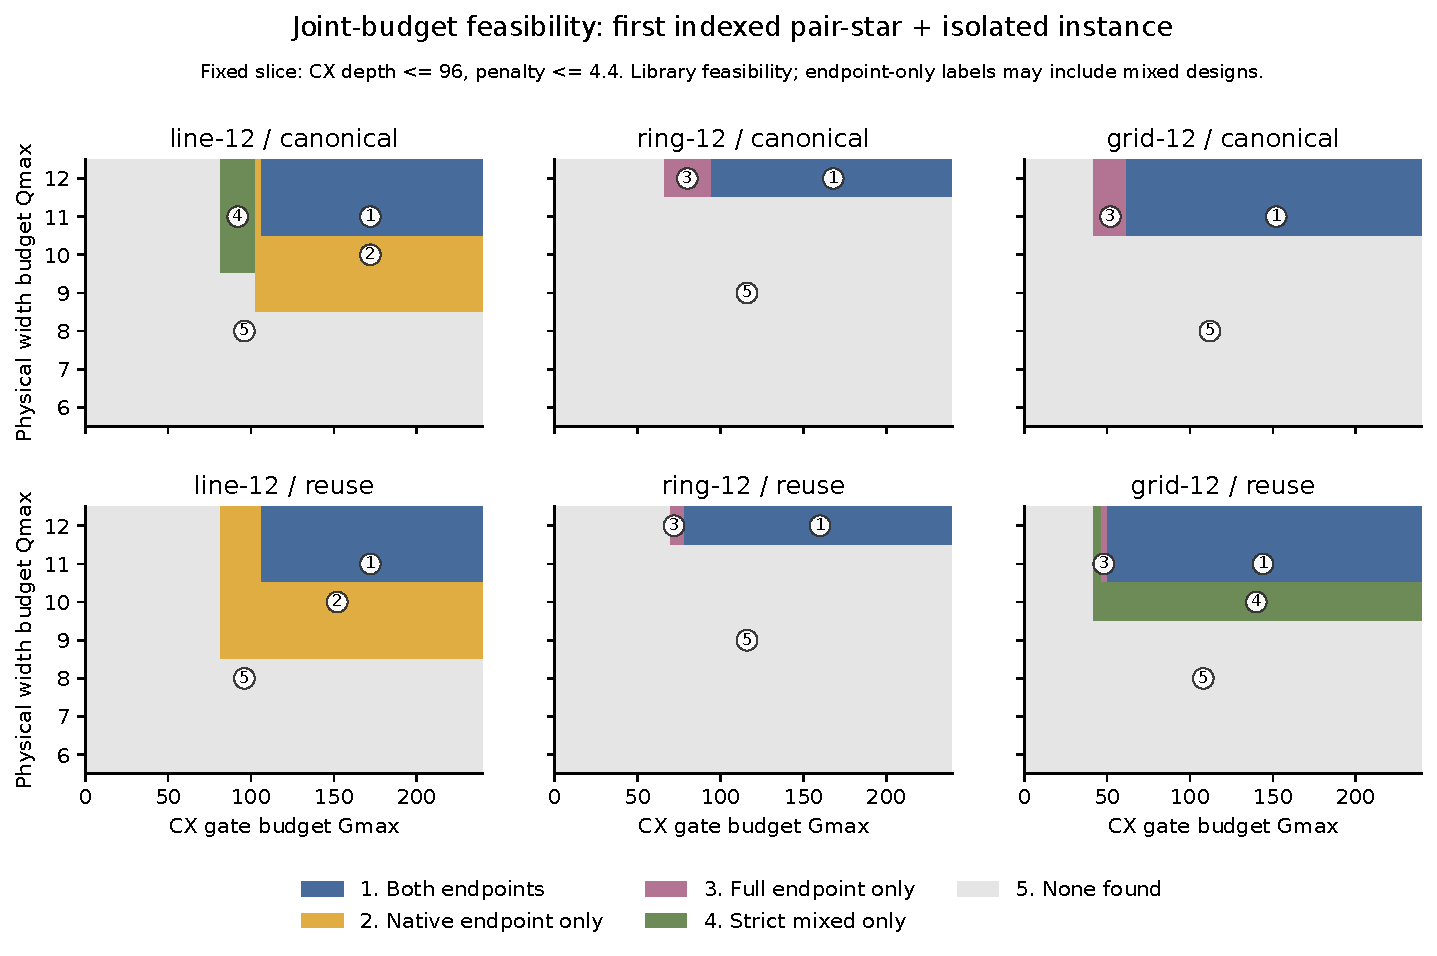
\includegraphics[width=\textwidth]{joint_budget_phase_map.pdf}
\caption{Real-compiler joint-budget phase maps for the first indexed
constructed instance at $D_{\max}=96$, $M_{\max}=4.4$. Width is physical
routing footprint. The same device capacity is used throughout. This is
an illustrative slice; population counts use the complete frozen grid.
The full endpoint is exhaustive over capacity-feasible assignments for
this constructed family; the mixed candidate library remains finite.}
\label{fig:new-joint-phase}
\end{figure*}

The first indexed constructed instance gives a concrete example.
Use ring-12 and canonical synthesis. The budgets are
$(Q_{\max},G_{\max},D_{\max},M_{\max})=(12,92,48,2.2)$.
The measured resource vectors $(Q,G,D,M)$ are:
\begin{itemize}
\item Native: $(12,96,55,0)$. Width fits, but gates and depth exceed the limits.
\item One full candidate: $(12,80,40,3.85)$. Width, gates and depth fit,
but penalty exceeds the limit.
\item One strictly mixed candidate: $(12,92,43,2.2)$. Every resource fits.
\end{itemize}
Checking one full candidate would not exclude the full endpoint.
We therefore check all full assignments. Every one with logical width at
most 12 has $M_{\max}\ge2.475$. The others exceed width.
Thus every full assignment fails, while the displayed mixed candidate fits.
Recompilation reproduces all three circuit records.

We chose this example after seeing the results, within the unchanged grid.
It illustrates exact feasibility. It does not demonstrate better QAOA
solution quality.

The best strictly mixed candidate has lower $J_{\rm new}$ than the
resource-optimised full candidate on every instance in every setting.
However, allowing native in the search changes the answer.
The unrestricted search selects native in all random-instance settings
and in 173/180 constructed settings.

The weighted score therefore usually favours native in this study.
The reason to use mixed is the joint hard budgets: they can exclude native
even when native has a lower weighted score.
The matched random control sometimes equals or beats the selected mixed
candidate. Our finite search does not guarantee that the chosen mixed
candidate is the best in its matching class.

Changing synthesis can change representation rankings.
We compare canonical and reuse scores on the same candidate identities.
The median Spearman correlations on line, ring and grid are
$0.913,0.915,0.949$ for Max3SAT; $0.906,0.905,0.955$ for cubic spin;
and $0.771,0.729,0.812$ for the constructed family.
A correlation near one means that the score rankings mostly agree.

We also compare the Pareto sets in $(Q,G,D,M)$.
A candidate is Pareto optimal within the library if no other candidate is
no worse in every resource and better in at least one.
Jaccard similarity measures the shared fraction of two Pareto sets.
Its median values on line, ring and grid are $0.333,0.250,0.333$ for Max3SAT;
$1,1,1$ for cubic spin; and $0.321,0.351,0.355$ for the constructed family.

The winning full assignment changes on 6--14 of 30 Max3SAT instances,
10--13 of 30 spin instances and 0--4 of 30 constructed instances,
depending on topology. Similar overall rankings therefore need not give
the same frontier or winner.
The study uses 31,577 compiler calls and 32,760 scheduled candidate
evaluations before sharing repeated results. We independently check the
logical phases and routed-circuit semantics.


\subsubsection{What changes across five compiler seeds}
\label{sec:multiseed-robustness}
We repeated cost-layer compilation for the same 30 Max-3SAT and 30
constructed instances from the preceding study. These are reused
instances, not 60 new independent samples. We kept each target's candidate
library fixed and tested five routing seeds, three 12-qubit topologies and
both synthesis strategies. All 101,460 planned compilations completed.
The new run fixes eight SABRE trials. The earlier run used different
effective routing settings, so we establish a new seed-1729 baseline.
Methods in Section~\ref{sec:multiseed-methods} give the full comparison.

Here a budget point is \emph{mixed-only within the library} when an exact
strictly mixed candidate meets all four limits, while every native or
fully reduced candidate in that library fails at least one limit.
This test does not exclude full reductions outside the library.
It is therefore different from the exhaustive width/penalty certificate
in the preceding subsection.

The new baseline has 149,439 such points across all instance, topology and
synthesis settings. Of these, 79,069 remain mixed-only under every tested
seed: a retained fraction of 52.91\% ($79{,}069/149{,}439$).
The same budget point must pass in all five seeds, but the feasible mixed
candidate may change with the seed. This count does not prove that one
candidate works for all five seeds. Budget points share instances and are
not independent observations.
Of the 360 instance--topology--synthesis settings, 49 retain every
baseline TRUE point, 171 retain some but not all, 35 retain none of a
nonempty baseline, and 105 have an empty baseline. Retaining every
baseline point does not require identical regions: other seeds may gain
new TRUE points. Supplementary Section~\ref{supp:multiseed-results} gives the results by
family and topology, the changes in selected candidates and the corrected
seed-by-seed display. Mixed-only budget points can survive these five
seeds, but a substantial part of the baseline region does not.

\subsubsection{Fresh evaluation: preparation and incremental evolution}

\label{sec:fresh-qaoa}

The new QAOA study separates preparation from evolution.
We freeze the code, seeds, hypotheses and budgets before generating data.
Each family has 30 new independent instances with $n=6$ and six clauses
or spin interactions. Sampling is uniform under two conditions: all variables
are covered, and at least two cubic monomials remain nonzero.
The study is small, noiseless and limited to $p=1$.
Its freeze is local, not externally registered.

The earlier 14-, 20- and 18-instance sets remain exploratory.
The signal-enriched set is a separate mechanism study.

We compare native, proper mixed ($0<|D|<|E|$) and full reduction.
Mixed and full selection use the same reference-compiler score
$J_{\rm res}=(a/4+G/160+D_2/120+M/8)/4$.
Each evaluates up to 128 distinct seeded candidates. If the domain is
smaller, we evaluate it completely. Penalties equal the cubic threshold
plus one. The fibre diagnostic is not used in selection.

The mixed comparison is conditional on using a proper mixed representation.
If native is allowed, it has the smallest resource score among evaluated
candidates on all 60 instances.
This selection uses the all-to-all reference compiler. It is separate from
the topology-specific compilation study. The two studies cannot establish
a joint hardware-and-quality threshold on the same instances.

Every $p=1$ equal-effort arm uses the same three parameter starts for an
instance. Each restart receives exactly 120 objective evaluations.
We run COBYLA first. If it stops early, we fill the remaining quota with
uniform parameter samples from a fixed common seed.
This is COBYLA plus quota completion, not 120 COBYLA iterations.

We minimise the exact original expectation $\mathbb E[f(x)]$.
We sum over auxiliary outcomes. Encoded energy is a separate diagnostic.
Starts are uniform on $[0,2\pi)\times[0,\pi)$.
We do not add $p=0$ as an optimiser candidate. Positive gain over $p=0$
is therefore not guaranteed by construction.

All representations use the same pair/triple McCormick--RLT relaxation.
Original-bit probabilities are clipped to $[0.05,0.95]$.
For pair warming, we clip the auxiliary pair moments to this interval.
For independence warming, we multiply the clipped original probabilities
and clip the result to the same interval.
Preparation and matched mixing otherwise use the same rules across arms.

Write $f_{\rm cold,0}$ for the cold initial expectation,
$f_{\rm warm,0}$ for the warm initial expectation, and
$f_{\rm warm,1}$ for the optimised warm $p=1$ expectation.
The total improvement is
\[
\begin{aligned}
f_{\rm cold,0}-f_{\rm warm,1}
&=\underbrace{f_{\rm cold,0}-f_{\rm warm,0}}_{\text{classical preparation gain}}\\
&\quad+\underbrace{f_{\rm warm,0}-f_{\rm warm,1}}_{\text{incremental evolution gain}}.
\end{aligned}
\]
Every representation has the same original-bit distribution at warm $p=0$.
Their original expectations are therefore equal.
Independent sampling from these clipped marginals has the same expectation.
We also report 2,048 actual samples per instance and deterministic rounding
of the raw relaxation marginals, with ties rounded to zero.
These controls measure preparation. They do not compare against a fully
optimised classical algorithm.

\begin{table}[t]\centering\small

\caption{New $n=6$ QAOA results, with 30 independent instances per family. Positive gain means a lower original objective. Intervals are paired 95\% bootstrap intervals from 10,000 instance resamples. Evolution uses pair auxiliary warming and $3\times120$ equal-effort evaluations. Native evolution gain is the prespecified primary QAOA comparison. The other intervals are descriptive.}

\label{tab:fresh-warm-gain}

\begin{tabular}{llcc}\toprule

Family & Gain & Mean [95\% interval] & Positive / 30\\\midrule

Weighted Max-3SAT & Preparation & 0.484 [0.279, 0.703] & 17 \\

Weighted Max-3SAT & Native evolution & 1.152 [0.959, 1.344] & 30 \\

Weighted Max-3SAT & Mixed evolution & 1.086 [0.900, 1.277] & 30 \\

Weighted Max-3SAT & Full-Q evolution & 0.778 [0.661, 0.891] & 30 \\

Cubic spin glass & Preparation & 0.000 [0.000, 0.000] & 0 \\

Cubic spin glass & Native evolution & 2.133 [2.004, 2.238] & 30 \\

Cubic spin glass & Mixed evolution & 1.222 [1.063, 1.376] & 30 \\

Cubic spin glass & Full-Q evolution & 0.648 [0.522, 0.780] & 30 \\

\bottomrule\end{tabular}\end{table}

\begin{figure}[t]\centering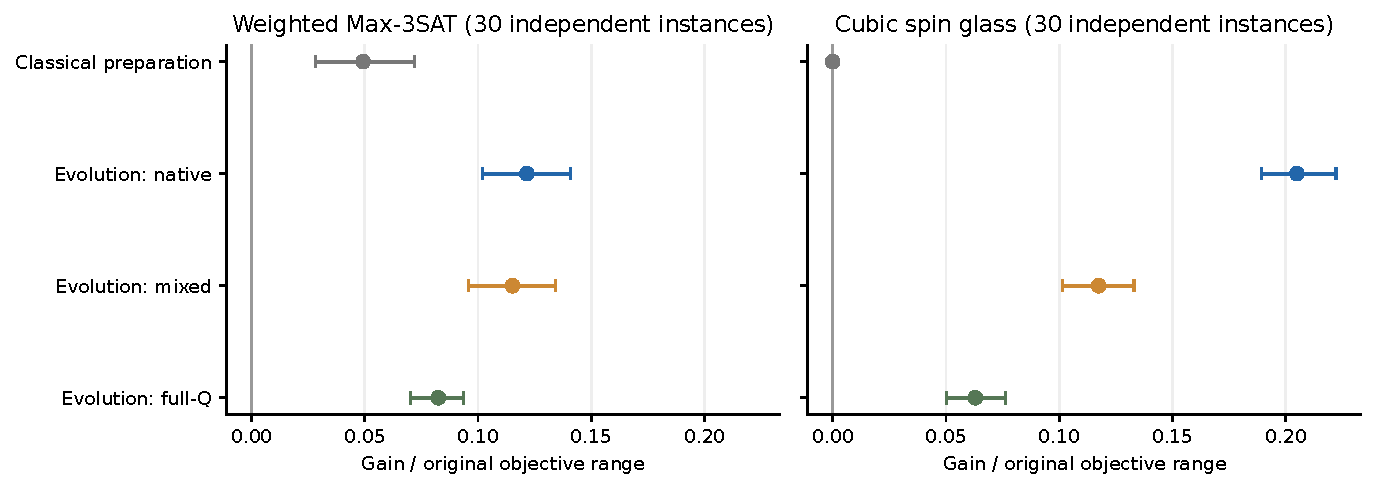
\includegraphics[width=\linewidth]{revision_warm_gain_decomposition.pdf}

\caption{Classical preparation and subsequent $p=1$ evolution on fresh instances. Each gain is divided by its instance's exact original-objective range before averaging. Bars are paired instance-bootstrap 95\% intervals; positive values reduce the original objective. The incremental bars use the same warm $p=0$ comparator.}\label{fig:fresh-warm-decomposition}\end{figure}

For weighted Max-3SAT, the mean preparation gain is 0.484 [0.279, 0.703].
Native evolution adds 1.152 [0.959, 1.344] beyond warm $p=0$.
The mean original objectives for raw rounding, independent sampling and
the prepared state are 2.267, 1.786 and 1.783.

Compared with independence warming, pair warming lowers the mean objective
by 0.046 [-0.005, 0.112] for proper mixed and 0.119 [0.040, 0.202] for full-Q.
The mixed interval includes zero. These are secondary results at a fixed
optimisation budget. They do not establish a general pair-moment benefit.

For cubic spin glass, the mean preparation gain is 0.000 [0.000, 0.000].
Native evolution adds 2.133 [2.004, 2.238] beyond warm $p=0$.
The mean original objectives for raw rounding, independent sampling and
the prepared state are -1.467, 0.010 and 0.000.

Compared with independence warming, pair warming changes the mean objective
by gains of -0.051 [-0.175, 0.061] for proper mixed and
0.112 [-0.011, 0.238] for full-Q. Both intervals include zero.
The spin data do not establish a pair-moment benefit.

\paragraph{Larger optimisation budgets.}
We also scan a $65\times65$ grid over the full $(\gamma,\beta)$ domain.
We then run four Nelder--Mead refinements, each with a 240-evaluation quota.
This gives 5,185 evaluations per warm pair arm.
If refinement stops early, the same uniform completion rule fills its quota.
The encoded energies are integers, so the $2\pi$ phase period is valid.
The zero-phase grid row includes the $p=0$ expectation.

A second equal-effort comparison uses Nelder--Mead with the same three
starts and $3\times120$ evaluations.
These checks show how results depend on optimisation effort.
The scan and local refinements do not prove a global optimum.

\begin{table}[t]\centering\small\caption{Mean original objectives with pair warming. EE uses equal-effort COBYLA with quota completion. NM uses equal-effort Nelder--Mead. Scan uses a $65^2$ grid and local refinement. Lower is better.}\label{tab:fresh-optimizer}

\begin{tabular}{llrrr}\toprule Family & Representation & EE & NM & Scan\\\midrule

Weighted Max-3SAT & Native & 0.631 & 0.772 & 0.405 \\

Weighted Max-3SAT & Proper mixed & 0.697 & 0.799 & 0.533 \\

Weighted Max-3SAT & Full-Q & 1.005 & 1.057 & 0.891 \\

Cubic spin glass & Native & -2.133 & -1.979 & -2.257 \\

Cubic spin glass & Proper mixed & -1.222 & -1.228 & -1.495 \\

Cubic spin glass & Full-Q & -0.648 & -0.535 & -0.888 \\

\bottomrule\end{tabular}\end{table}

Of 172,800 equal-effort evaluations, 17,959 are uniform quota-completion
samples. The second optimiser uses no completion samples.
The scan-refinement stage uses 4,681.
We retain all traces, early-stop messages and evaluation counts.

For weighted Max-3SAT, increasing effort from COBYLA to scan refinement
changes the winning representation on 7/30 instances.
The mean within-instance rank correlation is 0.717.
Replacing COBYLA with equal-effort Nelder--Mead changes the winner on 9/30.
One optimiser and one budget do not give a stable ranking for every instance.

For cubic spin glass, scan refinement changes the COBYLA winner on 1/30
instances. The mean within-instance rank correlation is 0.917.
Equal-effort Nelder--Mead changes the winner on 2/30.
The ranking is more stable here, but still depends on the protocol.

\begin{figure}[t]\centering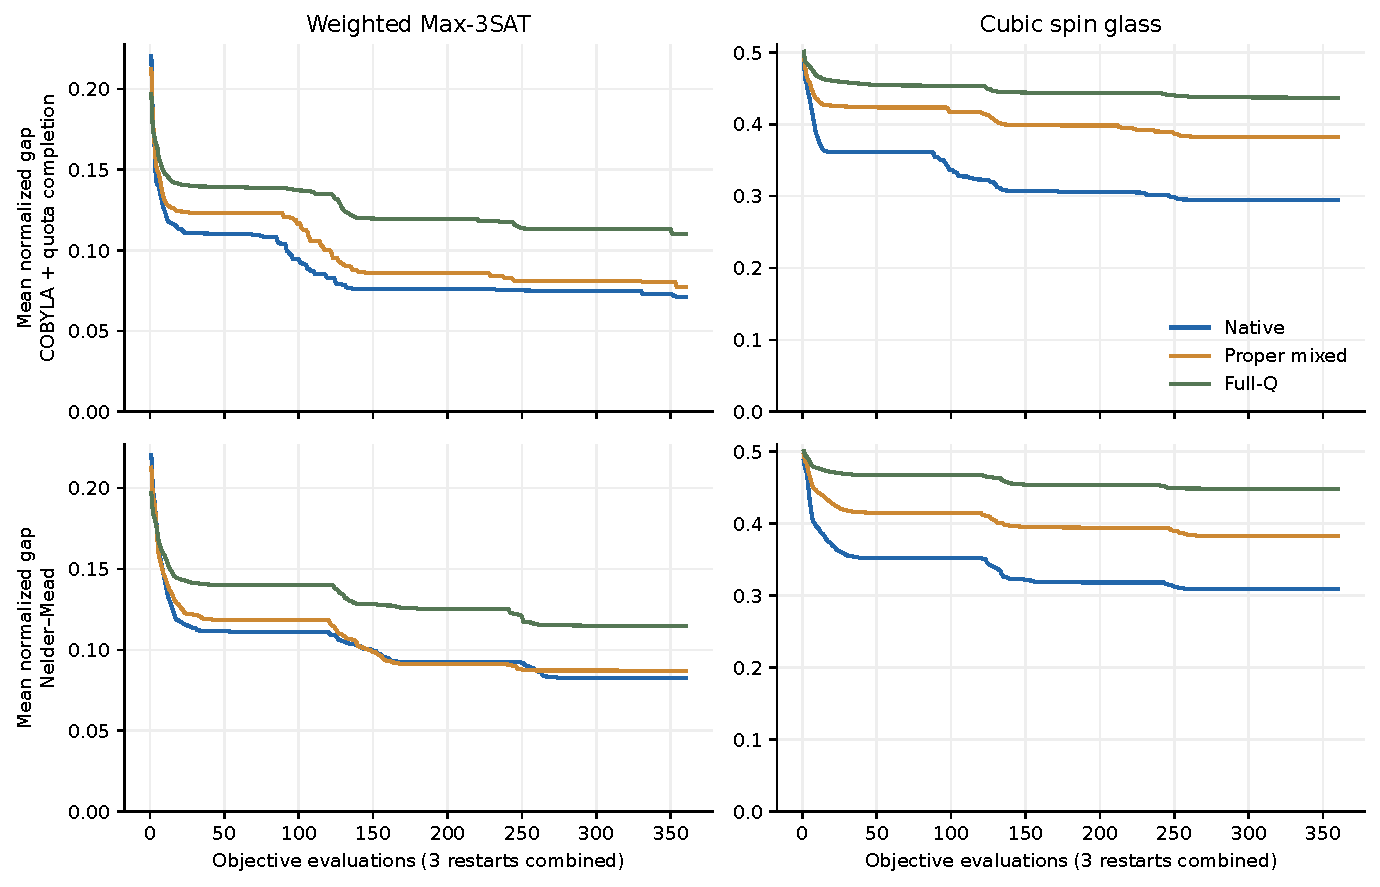
\includegraphics[width=.92\linewidth]{revision_optimizer_curves.pdf}

\caption{Incumbent original-objective gap, divided by each instance's exact objective range, versus cumulative evaluations over three restarts. Each line averages 30 independent instances. All curves use pair warming. They distinguish equal-effort behaviour from the separately reported larger scan-and-refinement budget.}\label{fig:fresh-optimizer-curves}\end{figure}

The new study uses independent instances and measures preparation and
evolution separately. Its scope is small noiseless $p=1$ simulation.
It does not show a solution-quality advantage for mixed representations or
a scalable quantum advantage.
This study does not test diagnostic prediction. The separate joint study
below addresses that question and distinguishes prediction from selection.

\subsubsection{Joint resource and solution-quality test}
\label{sec:feedback-iteration-v3}\label{sec:v3-joint}
The first two studies use different instances and circuit scopes. We therefore
ran a third study that checks resources and quality on the same circuit.
Its protocol and source hashes were saved before instance generation.
This is a local freeze, not external preregistration.
There are 30 new Max-3SAT and 30 new cubic-spin instances with six original
bits. A separate set has 12 nine-bit pair-star mechanism instances.
All 72 objectives are distinct, with no exact overlap with 462 supplied
historical objectives. We analyse the three cohorts separately.

We compile the complete symbolic $p=1$ circuit, including preparation,
cost evolution and the matched mixer. The target is ring-12, with reuse
synthesis and the fixed Qiskit level-3 settings.
Full and proper-mixed selection use the same score in
Eq.~\eqref{eq:new-compiled-score} and matched candidate quotas.
Selection does not use QAOA outcomes. Each evaluated design uses three
common starts and 120 Nelder--Mead evaluations per start, including the
declared quota completion. Key designs, chosen before observing quality,
also receive a $65^2$ scan and four local refinements.
Section~\ref{sec:v3-methods} gives the protocol.

\paragraph{The primary test.}
The fixed resource limits are $(Q,G,D,M)\leq(12,96,64,16)$.
We measure quality on the original bits using the normalised gap
\begin{equation}
g=\frac{\mathbb E[f]-\min f}{\max f-\min f}\leq0.2.
\label{eq:v3-gap}
\end{equation}
The extrema are found by exact enumeration for these small instances.
Table~\ref{tab:v3-primary} reports resource availability and joint success
separately. Quality in the primary test uses the scan-refined results.
No instance has mixed-only joint success at this primary budget.
This is a negative result for the primary question.

\begin{table}[htbp]\centering\small
\caption{Primary test. Each entry is the number that fits the resource
budgets followed by the number that also meets $g\leq0.2$.
Mixed-only joint success is zero in every cohort.}
\label{tab:v3-primary}
\begin{tabular}{lrrrr}\toprule
Cohort & $N$ & Native & Full & Proper mixed\\\midrule
Max-3SAT & 30 & $30\to30$ & $8\to7$ & $30\to30$\\
Cubic spin & 30 & $30\to1$ & $0\to0$ & $30\to0$\\
Mechanism & 12 & $9\to9$ & $12\to12$ & $12\to12$\\\bottomrule
\end{tabular}\end{table}

Zero observed successes do not prove a zero population rate.
The one-sided 95\% binomial upper limits are 9.50\% for $0/30$ and
22.09\% for $0/12$. Resampling all-zero counts gives a degenerate
bootstrap interval and does not resolve this uncertainty.

\paragraph{The secondary budget grid.}
The frozen secondary grid has 432 resource-budget combinations and quality
targets $0.1,0.2,0.3$. At $g\leq0.2$, at least one cell has only the selected
mixed design jointly successful for 7/30 Max-3SAT, 0/30 spin and 5/12
mechanism instances. These are instance counts, not independent cell trials.
For 3/30, 0/30 and 4/12 instances, respectively, the evidence is stronger:
native fails compiled resources, and exhaustive logical width/penalty checks
exclude every full assignment in the stated grammar.
Failure of one selected full design alone would not establish that result.

\begin{table}[htbp]\centering\small
\caption{Secondary grid at $g\leq0.2$. Counts refer to independent instances
with at least one qualifying cell. The last column also requires native
resource failure and exhaustive resource exclusion of every full assignment.}
\label{tab:v3-secondary}
\begin{tabular}{lrrr}\toprule
Cohort & $N$ & Selected mixed only & Full endpoint excluded\\\midrule
Max-3SAT & 30 & 7 & 3\\
Cubic spin & 30 & 0 & 0\\
Mechanism & 12 & 5 & 4\\\bottomrule
\end{tabular}\end{table}

\paragraph{One verified example.}\label{par:v3-witness}
We chose \texttt{max3sat\_07} after examining the results, within the
unchanged secondary grid. Its budget is $(8,64,64,8)$.
Native uses $(Q,G,D,M)=(6,65,50,0)$, so it exceeds the CX limit.
All 729 full pair assignments need at least nine logical qubits, so they
exceed width. A selected mixed circuit uses $(7,58,36,7)$ and meets
every resource limit. Its equal-effort gap is $0.1848065782$, below $0.2$;
its warm $p=0$ gap is $0.25$. The saved-angle expectation was independently
reproduced with the transpiled circuit statevector.

This example establishes conditional joint feasibility under this compiler,
grammar and budget. It does not change the zero primary result.
The best of 2,048 classical samples has gap zero on this instance.
Across all cohorts, the best classical sample meets $g\leq0.2$ on every
instance. A best sample and a circuit expectation are different quantities.
The comparison does not establish quantum advantage.

\paragraph{Optional fibre diagnostics.}\label{sec:v3-guardrail}
The no-guardrail, raw-moment and clipped prepared-state rules choose the
same design on all 72 instances. The tested guardrails therefore give no
observed selection benefit. We also test prediction on instances not used
to fit the prediction model. The diagnostic helps predict final auxiliary
inconsistency, but its benefit for final objective quality is uncertain.
Better prediction does not show that a threshold improves selection.
The guardrail remains optional.
Supplementary Section~\ref{supp:v3-diagnostics} gives the results.

The study used 4,560 main compiler calls and 1,476,585 objective evaluations.
Checks reproduce saved states and diagnostics; they do not rerun all
optimisation. The Windows audit finds two total-gate-count differences,
while all checked budget and score fields match.
Appendix~\ref{app:v3-portability} preserves the strict replay failure and
the separate compatibility result. These are small noiseless simulations
under one compiler configuration.

\subsubsection{What the earlier studies establish}
The earlier studies helped develop and check the method. They are not part
of the fresh evaluation sets. Max-3SAT showed the clearest circuit savings;
spin glass showed a gate--depth trade-off. Native had the best mean objective
in the historical 14-instance QAOA comparison
(Supplementary Table~\ref{tab:e3-qaoa-summary}). The 20-instance signal-enriched
warm-start study does not establish a general pair-moment advantage.
The 18-instance noise test is exploratory and is not a calibrated hardware
test. Supplementary Section~\ref{supp:historical} reports these studies.

\section{Discussion}
\label{sec:discussion}\label{sec:conclusion}\label{sec:discussion-search-scope}
The main result is that mixed can be the only feasible exact representation.
The static theorem needs no compiler. Corollary~\ref{cor:compiled-star-isolated}
also includes gates and depth, but only under its stated synthesis $\Pi$.
Its proof lists every contributing Pauli support and derives the CNOT layers.
It is a count for this circuit, not a lower bound for every possible circuit.
Both results concern the direct semantic pair-substitution grammar.
They do not exclude other quadratization constructions.

The measured circuits show the same resource mechanism on sparse devices.
Native can fail gates or depth while all full assignments fail width or
penalty, leaving a feasible mixed design. This depends on the synthesis
and target. Reuse synthesis removes the observed spin mixed-only regions.
Similar score rankings can still give different Pareto sets and winners.
Selection should therefore be repeated for the device and synthesis in use.


The five-seed follow-up gives a further limit on compiler robustness.
Within its saved candidate libraries, 52.9\% of the new seed-1729
mixed-only budget points remain mixed-only in all five seeds.
The feasible candidate may differ between seeds. This supports the
existence of shared feasible budget regions in the tested settings,
but not a claim that every region or every selected representation is
stable. It also does not exclude representations outside the libraries.

Hard budgets and weighted scores answer different questions. Native has the
lowest unrestricted score in every random-instance setting of the compiler
study. Mixed becomes useful when a hard budget excludes native.
The separate QAOA study also favours native on mean original-objective
quality under equal effort, a second optimiser and a larger parameter scan.
Some instance winners change with effort. Exactness and smaller circuits
do not determine QAOA quality. Earlier work on local structure and constraint
density motivates this caution~\cite{WangMaxCut2018,FarhiLocal2020,Akshay2020}.

The third study tests resources and quality together. Its primary mixed-only
counts are $0/30$, $0/30$ and $0/12$. A fixed secondary grid contains conditional
successes, including the verified \texttt{max3sat\_07} example. This is evidence
for existence at particular budgets, not a positive primary result or a
general quality advantage. The best classical sample meets the quality
target on every instance, so no quantum advantage is established.

Warm-start gains have two sources. The fresh study measures classical
preparation and subsequent evolution separately. Native evolution improves
on warm $p=0$ on all 30 instances of each family under the equal-effort
protocol. Pair warming has no benefit that holds across both families and
all representations. The signal-enriched old study is a separate mechanism
test. It cannot represent ordinary random instances. Results for standard
QAOA started at a classical string~\cite{Cain2023} also do not directly apply
to our matched product-state mixer.

The fibre study tests prediction and selection separately. After including
the stated control variables, adding the prepared-state diagnostic reduces
the mean squared prediction error for inconsistency by about 27.7\% on
held-out instances. The interval for better quality prediction includes
zero. All three guardrail rules select the same designs. These results do
not show that using the threshold improves the algorithm.

The historical 14-, 20- and 18-instance studies remain exploratory and are
reported in the Supplementary Information. Different device capacities
cannot isolate connectivity alone. A $p=0$ row measures a budget limit,
not completed positive-depth optimisation. A smaller noise-induced loss
from a worse noiseless starting value need not give a better final value.
The old coordinate correction and numerical environment changes also
prevent attributing every change to the mixer convention alone.

The supported contribution is resource-constrained exact representation
selection. The data are small and noiseless. Finite search returns the best
design found; only a stated exhaustive certificate proves optimality or
infeasibility. The primary and secondary tests, and the three fresh cohorts,
must stay separate. Larger studies should test higher-degree search,
additional compilers and positive-depth quality under tight hardware budgets.

\section{Methods}
\label{sec:methodology}
\label{sec:experiments}

\subsection{Resource-aware selection and certification}
\label{sec:selection}
\label{sec:selection-problem}
\label{sec:search-certification}

First fix a compilation protocol $\Pi$. Specify the device, synthesis,
compiler seeds and aggregation rule. Then choose positive resource scales
and nonnegative weights that sum to one. The score is
\begin{equation}
J_{\mathrm{res}}(\sigma)=
w_a\frac{a_\sigma}{s_a}+w_G\frac{G_{2q,\sigma}}{s_G}
+w_D\frac{D_{2q,\sigma}}{s_D}+w_M\frac{M_{\max,\sigma}}{s_M}.
\label{eq:Jres}
\end{equation}
The compiler supplies gate count and depth. Polynomial degree alone does
not determine them~\cite{Verchere2023,Weidenfeller2022,Schmidbauer2024}.
Primary selection uses resource constraints only.
We compile candidates on the target being tested.
Old all-to-all certificates still validate the old model.
New finite-budget searches are heuristics unless we explicitly give an
exhaustive certificate.

We keep the fibre excess only as an optional diagnostic
(Appendix~\ref{app:fibre-risk}). It measures the expected extra encoded
energy from the auxiliary assignments:
\begin{equation}
E_{\mathrm{fib}}(\sigma;\eta,\xi)=\mathbb E[F_\sigma(X,Y)-f(X)]\geq0,
\qquad \widehat E_{\mathrm{fib}}=E_{\mathrm{fib}}/s_{\mathrm{fib}}.
\label{eq:fibre-excess-short}
\end{equation}
Here all bits are independently Bernoulli with parameters $(\eta,\xi)$.
The scale $s_{\mathrm{fib}}>0$ is the same for every design.
Raw relaxation moments and clipped preparation probabilities give different
product laws. This definition does not claim that raw moments come from
one joint distribution.

The joint study tests whether this diagnostic adds predictive information
beyond auxiliary count, compiled score, reduced-term count, prepared-state
gap and family. It finds a limited benefit for predicting inconsistency
on held-out instances. The benefit for predicting quality is uncertain,
and the tested thresholds do not change the selected designs. Primary
resource selection therefore does not use this diagnostic.

Keep only exact representations that meet all four budgets:
\begin{equation}
\mathcal F_{\mathrm{sel}}=\left\{\sigma\in\Sigma_{\mathrm{ex}}^\varepsilon:
\begin{array}{c}
N_\sigma\leq Q_{\max},\ G_{2q,\sigma}\leq B_G,\ D_{2q,\sigma}\leq B_D,\\
M_{\max,\sigma}\leq B_M
\end{array}\right\},
\label{eq:selection-feasible-set}
\end{equation}
Then minimise the score over that set:
\begin{equation}
J_{\mathrm{res}}^\star=\min_{\sigma\in\mathcal F_{\mathrm{sel}}}J_{\mathrm{res}}(\sigma).
\label{eq:selection-problem}
\end{equation}
The set is finite, so a minimum exists if it is nonempty.
To test the freedom to retain terms, compare full search with selective search:
\begin{equation}
\min_{\rho:(E,\rho)\in\mathcal F_{\mathrm{sel}}}J_{\mathrm{res}}(E,\rho)
\quad\hbox{with}\quad
\min_{\mathcal D,\rho:(\mathcal D,\rho)\in\mathcal F_{\mathrm{sel}}}J_{\mathrm{res}}(\mathcal D,\rho).
\label{eq:fair-full-comparison}
\end{equation}
Every full representation is also selective. Exact search over the larger
family therefore cannot have a worse best score.
Finite searches may miss different candidates, so this ordering need not
hold for their returned designs. We report best-found scores and compiler
calls rather than calling them global optima.

Minimum-auxiliary full reduction tests a different resource objective.
Maximum reuse tests a simple structural rule.
A device-aware rule tests the value of device information.
Random controls matched on $a_\sigma$ and $|\mathcal D|$ compare choices
with the same two counts. Those matches alone do not fix penalty or reuse.

\begin{figure}[tbp]
\centering
\begin{tikzpicture}[
  x=\textwidth,y=1cm,
  font=\footnotesize,
  box/.style={draw=black!65,rounded corners=2pt,fill=black!2,
    align=center,text width=.265\textwidth,inner sep=5pt,
    minimum height=1.02cm},
  result/.style={box,fill=blue!4,draw=blue!55!black},
  decision/.style={diamond,aspect=2.3,draw=black!65,
    fill=black!2,align=center,inner sep=3pt},
  arr/.style={-{Stealth[length=2mm,width=1.4mm]},thick,draw=black!75}
]
\node[box] (input) at (.165,0)
  {\textbf{Fix the problem}\\
   Exact family and protocol\\Score and budgets};
\node[box] (seed) at (.5,0)
  {\textbf{Evaluate references}\\
   Native and fully reduced\\Update feasible incumbent};
\node[box] (beam) at (.835,0)
  {\textbf{Pareto-beam search}\\
   Score completions\\Keep up to $B$ prefixes};
\node[decision] (certify) at (.835,-1.65)
  {Certify?};
\node[box] (bnb) at (.5,-1.65)
  {\textbf{Branch and bound}\\
   Root frontier; reuse records\\Admissible pruning only};
\node[result] (certified) at (.5,-3.25)
  {\textbf{Return design / status}\\
   Certified bounds\\Gap, if bounds are finite};
\node[result] (heuristic) at (.835,-3.25)
  {\textbf{Return heuristic result}\\
   Incumbent, if found\\No optimality certificate};
\draw[arr] (input) -- (seed);
\draw[arr] (seed) -- (beam);
\draw[arr] (beam) -- (certify);
\draw[arr] (certify) -- node[above,font=\scriptsize]{yes} (bnb);
\draw[arr] (certify) -- node[right,font=\scriptsize]{no} (heuristic);
\draw[arr] (bnb) -- (certified);
\end{tikzpicture}
\caption{Representation selection separates a practical search from optional
certification. The beam seeks a low-cost feasible design; its discarded
prefixes remain part of the certification search. Branch and bound may
return an optimal, infeasible or interrupted status, with bounds reported
according to the stopping rules in Appendix~\ref{app:selection-implementation}. The historical optional fibre constraint is not part of the primary selector.}
\label{fig:selector-workflow}
\end{figure}

Each cubic term can stay native or use one of three pairs.
This gives a finite search tree. A Pareto beam keeps at most $B$ prefixes
at each step and records the best feasible design found so far.
We call that design the \emph{incumbent}.
Discarding prefixes can miss better designs.

Optional branch and bound~\cite{LandDoig1960,LawlerWood1966} starts again
from the root and reuses completed evaluations.
It removes a subtree only after proving it infeasible or proving its score
cannot improve the incumbent. A failed native completion alone is not
such a proof: a descendant may reduce more terms and become feasible.

Let $U_J$ be the score of the best feasible evaluated design.
Each unresolved subtree has a valid lower score bound.
Let $L_J^{\mathrm{glob}}$ be the minimum of these bounds and $U_J$.
The frontier must still cover every unresolved design.
If a feasible incumbent exists, then
\begin{equation}
L_J^{\mathrm{glob}}\leq J_{\mathrm{res}}^\star\leq U_J,
\qquad U_J-J_{\mathrm{res}}^\star\leq U_J-L_J^{\mathrm{glob}}.
\label{eq:anytime-certificate}
\end{equation}
The left inequality is a lower bound on the best possible score.
The right inequality follows because the incumbent is feasible.
Their difference bounds how far the incumbent can be from the optimum.

Equal bounds certify the optimal value only for the stated design space,
compiler and constraints. Without an incumbent, we report that no feasible
design has yet been found. We claim infeasibility only after exhausting
the frontier.
Figure~\ref{fig:selector-workflow} shows the procedure.
The old optional fibre check in Algorithm~\ref{alg:selector} is disabled
for primary selection.
Appendix~\ref{app:certified-selection} gives the bounds and numerical rules.
The proof of Proposition~\ref{prop:anytime-certificate} checks each part
of the interval separately.

\subsection{Warm-started QAOA and evaluation}
\label{sec:warm-start}
\label{sec:warm-start-state}
\label{sec:ws-qaoa}
\label{sec:cost-consistency}

For each representation, use the same relaxation to prepare a product
warm start~\cite{Egger2021,TateSDP2023,TateCustom2023}.
Clip original marginals by setting $\mu_i=\operatorname{clip}_\delta(\bar\mu_i)$,
where $\operatorname{clip}_\delta(t)=\min\{1-\delta,\max\{\delta,t\}\}$
and $0<\delta<1/2$.

The historical pair rule uses
$q_p=\operatorname{clip}_\delta(\bar q_{ij})$.
Its independence fallback uses $q_p=\mu_i\mu_j$ without clipping again.
The new QAOA study in Section~\ref{sec:fresh-qaoa} clips both auxiliary
rules to the same interval. This is a stated difference between protocols.

Let $|\phi(t)\rangle=\sqrt{1-t}|0\rangle+\sqrt t|1\rangle$.
The product state is
\begin{equation}
|\Phi_\sigma^{\mathrm{ws}}\rangle=
\bigotimes_{i=1}^n|\phi(\mu_i)\rangle
\otimes\bigotimes_{p\in P_\rho}|\phi(q_p)\rangle.
\label{eq:ws-state}
\end{equation}
For its ordered probabilities $\omega=(\mu,q)$, use the matched mixer
\begin{equation}
H_{M,\sigma}^{\mathrm{ws}}=\sum_{j=1}^{N_\sigma}h_M^{(j)}(\omega_j),
\qquad h_M(t)=-2\sqrt{t(1-t)}X-(1-2t)Z.
\label{eq:ws-mixer}
\end{equation}
The warm state is the unique ground state of this mixer Hamiltonian.
Use $U_F(\gamma)=e^{-i\gamma H_{F_\sigma}}$ and
$U_M(\beta)=e^{+i\beta H_{M,\sigma}^{\mathrm{ws}}}$.
If every qubit has probability $1/2$, then
$H_{M,\sigma}^{\mathrm{ws}}=-\sum_jX_j$.
Thus $U_M(\beta)=e^{-i\beta\sum_jX_j}$, the cold mixer at the same angle.

After $r$ layers, the state is
\begin{equation}
|\psi_{r,\sigma}\rangle=
U_M(\beta_r)U_F(\gamma_r)\cdots U_M(\beta_1)U_F(\gamma_1)
|\Phi_\sigma^{\mathrm{ws}}\rangle,
\label{eq:method-qaoa-ansatz}
\end{equation}
At $r=0$, it is the prepared state.
All cost terms commute, so splitting the cost layer into phase gadgets is
exact. The local mixer can leave the correct-auxiliary subspace.
Penalties do not force every measurement to satisfy the auxiliary relations.
Mixers that preserve a feasible subspace are another possible
choice~\cite{Hadfield2019}.

We score QAOA using the original objective:
$\mathcal E_f(\psi)=\sum_{x,y}f(x)p_\psi(x,y)$, where
$p_\psi(x,y)=|\langle x,y|\psi\rangle|^2$.
Every auxiliary outcome contributes to this sum.
Optimum probability also sums over all auxiliary outcomes.

We record auxiliary inconsistency separately as
$R_{\mathrm{inc}}=\mathbb P_\psi(Y\neq\phi_\rho(X))$.
It is zero when there are no auxiliaries.
Appendix~\ref{app:warm-start-circuits} gives the circuit identities and
diagnostic definitions. The protocol below specifies budgets and aggregation.

\subsection{Benchmark construction and comparison protocol}
\label{sec:benchmark-protocol}

Weighted Max-3SAT minimises violated-clause weight:
\begin{equation}
 f_{\mathrm{3SAT}}(\bm x)=\sum_C w_C\prod_{\ell_i\in C}u_{\ell_i}(x_i),
 \qquad w_C>0,
 \label{eq:methods-max3sat}
\end{equation}
The factor is $u_{x_i}=1-x_i$ for a positive literal and
$u_{\neg x_i}=x_i$ for a negative literal.
A clause product is one exactly when every literal is false.
The spin-glass benchmark uses
\begin{equation}
 E(\bm s)=\sum_{\{i,j,k\}\in\mathcal E}K_{ijk}s_is_js_k,
 \qquad s_i\in\{-1,1\},\quad K_{ijk}\in\{-1,1\},
 \label{eq:methods-cubic-spin}
\end{equation}
Here $\mathcal E$ is the sampled set of triples.
Set $s_i=1-2x_i$, expand the products and combine equal monomials before
reduction. Sampling changes sparsity and pair reuse.
These two families provide different test problems. They do not isolate
application type from hypergraph structure.
Appendices~\ref{app:benchmark-generation}, \ref{app:max3sat}
and~\ref{app:spin-glass} give the generators and expansions.

The old evaluation has three tiers: 60 oracle instances, 180 compilation
instances and 14 test-labelled noiseless QAOA instances.
Each tier is balanced between families.
Oracle checks compare $f(\bm x)$ with $\min_{\bm y}F_\sigma(\bm x,\bm y)$
for every assignment. They also test threshold failures and consistency.

Separate studies use 18 noise instances and 20 strongest-screened warm-start
instances. Warm-start screening uses only relaxation information.
It does not use QAOA outcomes. The screened set is not a representative
random sample and is not pooled with the original comparison.
Candidate-pool generation targets differ from the numbers actually evaluated.

Each old instance has native, full, selective and matched-random designs.
Full reduction uses a minimum-cardinality pair cover with deterministic
tie-breaking. Five seeded random controls match only active auxiliary count.
They may repeat and need not match circuit resources.
Appendix~\ref{app:experimental-controls} gives their construction.

Within each family and tier, the split labels are $60\%/20\%/20\%$
for training, validation and test. Settings use training and validation
rows, with no direct selector retuning on test-labelled rows.
However, the pool was available during protocol development.
We therefore treat these labels as exploratory, not as an untouched test.
Resource summaries pool all 180 compilation instances.

The old compiler study uses common synthesis settings and five transpiler
seeds on all-to-all coupling and a 12-qubit $3\times4$ grid.
It records width, two-qubit gates and depth, routing, penalties and
coefficient range. Width failures are recorded separately.
Paired device comparisons use only instances where all compared designs fit.
Additional line, ring and heavy-hex tests compare selective and random
designs. They do not rerun QAOA
(Appendices~\ref{app:hardware-compiler-protocol} and~\ref{app:reproducibility}).

Old QAOA runs use COBYLA~\cite{Powell1994}, three restarts, at most
60 evaluations per restart and tolerance $10^{-3}$.
The loss is the original expectation $\mathcal E_f$.
Encoded energy and consistency are diagnostics.
Initial angles have $\gamma\in[0,2\pi]$ and $\beta\in[0,\pi]$.
These intervals choose starts; they do not bound the optimiser.

Equal-layer comparisons use $p=1,2$.
For gate budget $B\in\{128,256\}$, let $g_\sigma>0$ be the median grid
gate count of one cost layer. Assign
\begin{equation}
 p_\sigma(B)=\left\lfloor B/g_\sigma\right\rfloor.
 \label{eq:methods-gate-budget}
\end{equation}
If no layer fits, keep the $p=0$ initial-state baseline without optimisation.
Report these counts separately, along with the subset where every design
fits at least one layer. The targeted warm-start study uses only $p=1,2$.

Primary QAOA results use exact statevector expectations.
The old E6 noise study instead uses 4096 shots per evaluation.
It applies representative depolarising and readout errors on the grid,
not a calibrated device model.
Starting from \cref{eq:methods-gate-budget}, it lowers depth until the
complete transpiled measured circuit fits the budget.
Comparisons use the resulting depth.
Both noise levels reuse noiselessly optimised parameters without
re-optimisation (Appendix~\ref{app:noise-protocol}).

\subsection{Joint-study protocol and statistical scope}\label{sec:v3-methods}
The joint study saves its protocol, source hashes and six dependency versions
before generating instances. The 30 Max-3SAT and 30 spin objectives use six
variables and uniform generation, with variable coverage and at least two
nonzero cubic supports. The 12 mechanism objectives use nine variables,
four pair-star leaves and one disjoint triple. Labels are permuted uniformly.
Cubic weights are sampled independently from $\{1,2,3\}$ and affine
coefficients from $\{-2,-1,0,1,2\}$. Their integer energies justify the
$2\pi$ cost-angle period. Penalties are the exact construction-specific
threshold plus one. Clipping uses $\delta=0.05$.

We compile the complete symbolic $p=1$ preparation, cost and matched-mixer
circuit on ring-12. Settings are reuse synthesis, Qiskit 2.5.2 level 3,
SABRE routing, identity initial layout, seed 1729 and basis
$\{R_Z,\mathrm{SX},X,\mathrm{CX}\}$. Width counts occupied input sites
and all sites touched by routing. This differs from the cost-layer-only
scope in Section~\ref{sec:fresh-compiled}.

The full and proper-mixed searches use the same candidate quota: the smaller
of 32 and the sizes of their capacity-feasible design spaces. The mechanism
quota is 27 in the initial freeze. Full candidates include assignments chosen
for minimum auxiliary count, maximum pair reuse and short ring distances.
Mixed candidates include groups that share a pair and prefixes of a reuse
ordering. For each budget, full and mixed search separately choose the
lowest score in Eq.~\eqref{eq:new-compiled-score}. Ties use lexicographic
actions. QAOA outcomes are not used to propose or select designs.

Every evaluated design uses three common parameter starts and 120
Nelder--Mead evaluations per start. If the optimiser stops early, seeded
uniform samples fill the remaining quota. Before observing quality, we
choose a set of designs for the larger scan. This set includes the native,
full and three guardrail choices made under capacity limits alone, together
with the full and mixed choices at the primary budget. Each distinct design
receives a $65^2$ grid and four refinements with 240 evaluations each.
If several choices give the same design, they share one evaluation.
The optimisation loss is the original expectation. Encoded energy and
auxiliary consistency are separate diagnostics. Classical controls are the
warm $p=0$ expectation, deterministic rounding of raw marginals, and the mean
and best of 2,048 independent samples.

The secondary grid is
\[
\begin{aligned}
Q_{\max}&\in\{8,10,12\},&G_{\max}&\in\{64,96,128,160,192,256\},\\
D_{\max}&\in\{32,64,96,128\},&M_{\max}&\in\{2,4,8,16,32,64\}.
\end{aligned}
\]
It has 432 cells, each checked at $g\leq0.1,0.2,0.3$.
Cells are correlated sensitivity checks, not independent trials.
We distinguish a failed selected endpoint from exhaustive resource exclusion
of all full assignments. The latter uses complete logical width/penalty
enumeration under the same grammar and penalty rule.

The optional raw/prepared guardrails use the same proper-mixed bank with
$Q\leq12$ and threshold $0.02$. The shared scale is
$4\sum_{p}(\sum_{e\supset p}|c_e|+1)$, summing all cubic pairs.
The raw rule uses relaxation moments; the prepared rule uses the clipped
probabilities actually used to prepare the state. An empty eligible set
is unavailable. We do not relax the threshold or insert a fallback.

For prediction, a fixed seed selects eight mixed candidates from each random
instance before outcomes are observed. This gives 480 probes. We fit a linear
model while leaving out all probes from one instance, then predict those
probes. We repeat this for each instance. The control variables are auxiliary
count, compiled score, reduced-term count, warm $p=0$ gap and family.
We add the raw and prepared diagnostics separately and together.
To form intervals, we resample the held-out errors by instance. We do not
refit every model in each resample. These intervals are secondary,
descriptive and unadjusted. Prediction does not test whether the threshold
causes better selection. Instances are the statistical unit. The 12 mechanism
instances are analysed separately from the random families. The two primary
guardrail comparisons for the random families use 10,000 paired instance
resamples and 97.5\% intervals.


\subsection{Five-seed compilation protocol}
\label{sec:multiseed-methods}
This follow-up reuses the Max-3SAT and constructed cohorts in
Section~\ref{sec:fresh-compiled}. It contains 30 instances from each
family and no cubic-spin instances. The smaller 10-per-family subset is
nested in this sample; it is not a second sample. Instances are ordered
by the saved SHA-256 selection rule.

For each instance and target, we use the saved full and mixed candidate
libraries from the earlier study. We do not add candidates after examining
the new seed results. There are 20,292 candidate--target--synthesis rows:
11,330 full, 8,602 strictly mixed and 360 native. Compiling each row at
seeds $\{1729,2718,31415,57721,65537\}$ gives 101,460 tasks.
The full search is not exhaustive for the Max-3SAT family.
All claims in this follow-up refer to the saved library.

The compiler is Qiskit 2.5.2 with basis
$\{R_Z,\mathrm{SX},X,\mathrm{CX}\}$ and optimisation level 3.
The targets are line-12, ring-12 and grid-12. Each uses canonical and reuse
synthesis. Initial placement is the identity. The explicit SABRE routing
pass uses the decay heuristic and eight trials. Placement search is
disabled. Thus the five seeds share the same routing settings.
The earlier archive used implicit routing settings. Its seed-1729 output
is not the control for this comparison: the new run supplies that control.

We use the same four-dimensional budget grid as in
Section~\ref{sec:fresh-compiled}. It has
$7\times61\times7\times7=20{,}923$ points per instance--target--synthesis--seed
setting. $Q$ counts occupied input sites and any extra sites used by
routing. $G$ counts CX gates, $D$ is CX-only depth, and $M$ is the largest
Rosenberg penalty coefficient. These resources cover one cost layer;
they exclude preparation and mixers. There is no quality threshold in
this follow-up.

At each point we first check candidate exactness and strict mixed status.
A point is TRUE when at least one such mixed candidate fits and no
non-mixed candidate in the library fits. It is FALSE when this condition
is ruled out by complete records. Missing evidence remains UNKNOWN;
we do not count it as failure or as zero resource use. All saved tasks
compiled successfully, and this run has no UNKNOWN points.
For a fixed instance, topology and synthesis, we intersect the five TRUE
sets. Retention is the size of this intersection divided by the size of
the seed-1729 TRUE set. Pooled retention uses sums of these two counts.
It is not the mean of the individual retention fractions.

For candidate rankings, we use $J_{\rm new}$ in
Eq.~\eqref{eq:new-compiled-score} with the active auxiliary count in its
width term. The archived selector is the lowest-score candidate within
device capacity, without the other hard limits. Ties use the candidate
identifier in lexicographic order. A changed winner and a changed feasible budget region
answer different questions. Supplementary
Section~\ref{supp:multiseed-results} reports both, and states the budgets
used for the added check of the baseline winner.
Appendix~\ref{app:multiseed-audit} records the checks and their limits.

\subsection{Use of language-model assistance}
Language-model assistance was used to edit the text, develop and review
code, and check proofs and saved numerical results. The archived protocols,
source hashes and verification records distinguish scientific runs from
later checks and editorial changes.

\subsection{Statistics and reproducibility}
\label{sec:statistics-reproducibility}

The independent statistical unit is an instance.
For old resource results, first take the median over transpiler seeds for
each design. Then average the five random-design values within the instance.
For old QAOA, first average three restarts per design. Then average the
random-design means. Finally, form paired differences within each instance.
We do not choose the best seed, restart or random draw.

Resource summaries use medians of paired differences.
Old QAOA, warm-start and noise summaries use means and two-sided 95\%
Student-$t$ intervals across instances~\cite{Student1908}.
The new studies use the aggregation and bootstrap rules stated in their
own protocols.

Corrected warm-start intervals use $n-1$ degrees of freedom.
They are exploratory and unadjusted for multiple comparisons.
An interval including zero does not establish equivalence.
Seeds and restarts do not add independent instances.
The descriptive regime labels use a separate endpoint-stability rule
(Appendix~\ref{app:experimental-statistics}).

The old warm-start correction keeps the frozen instances, designs,
probabilities, starts, seeds, budgets and loss.
It does not resolve the LP or screen new instances.
We rerun positive-depth cold controls because the optimiser environments
are not known to be equivalent. We validate reuse at zero depth.
Old and corrected outcomes are not pooled.

Original E4 uses the first HiGHS optimum.
Selection and targeted screening use a deterministic representative of the
LP optimum face. We preserve these different rules.
Appendices~\ref{app:experimental-lp},
\ref{app:optimisation-hyperparameters} and
\ref{app:warmstart-correction-provenance} give the solver and execution records.

\FloatBarrier
\section*{Data availability}
The new evaluation data, frozen protocols, execution records and analysis scripts
are supplied with this revision: the 17 September code-and-evidence archive,
\nolinkurl{URSS_Feedback_Iteration_v3.zip}, the Windows verification evidence,
and the five-seed delivery described in Appendix~\ref{app:multiseed-audit}.
The additional data corrections are supplied as a separate checked analysis.
The review package preserves these inputs and their SHA-256 identities.
The five-seed source and selected R12 acceptance evidence are available for
review in the repository's draft repair pull request; this does not imply
publication of the complete scientific data or adoption of this manuscript.
The historical
processed data and source manifests
are available in the
\href{https://github.com/rrocy6/Exact-mixed-locality-representation-selection-for-resource-constrained-QAOA}{project
repository}. The complete raw data for the warm-start coordinate correction are publicly
archived in the
\href{https://github.com/rrocy6/Exact-mixed-locality-representation-selection-for-resource-constrained-QAOA/blob/efaa1ce60fbc9984006472c4b2672578027fac78/delivery/20260913/archives/URSS_WARMSTART_CORRECTION_EXECUTED_v1.zip}{versioned correction archive}.
The archive identity and SHA-256 are recorded in
Appendix~\ref{app:reproducibility}.

\section*{Code availability}
The five-seed source snapshot and the independent correction script accompany
the additional results. The supplied snapshot has the coverage and environment
limits stated in Appendix~\ref{app:multiseed-audit}.

The resource and QAOA evaluation code and reproduction instructions are included with this revision. The v3 scientific freeze is preserved; the separate portability verifier, effective audit and explicit audit amendment are supplied with the Windows evidence described in Appendix~\ref{app:v3-portability}. Historical code, together with the
environment information and reproduction instructions, is available in the
\href{https://github.com/rrocy6/Exact-mixed-locality-representation-selection-for-resource-constrained-QAOA}{project
repository}.

\section*{Acknowledgments}
This work was supported in part by the National Hub for Edge AI,
UK Research and Innovation (UKRI), through Research Grant EP/Y028813/1;
by the UKRI Cross Council under Grant UKRI3734;
by the Academic Centre of Excellence in Cyber Security Research,
University of Warwick, under Grant EP/R007195/1;
and by the University of Warwick Undergraduate Research Support Scheme
(URSS).

\section*{Author contributions}
J.L. developed the idea and theoretical framework, proved the analytical
results and wrote the manuscript. Y.S. and R.Z. designed and implemented
the numerical experiments, analysed the data and helped interpret the
results. H.M.W., B.C. and C.M. provided research guidance and discussed
the work. The final submission remains subject to all authors' review
and approval.

\section*{Competing interests}
The authors declare no competing interests.

\appendix
\section{Background identities and resource definitions}
\label{app:background-details}

\subsection{Multilinear and Pauli expansions}
The same change between Boolean and spin variables is used in standard Ising
formulations~\cite{Lucas2014} and penalty-based QUBO
models~\cite{Glover2018}. Here it gives the Pauli terms that we compile when
we score each representation.

Every function $f:\mathbb B^n\to\mathbb R$ has the unique expansion
\begin{equation}
  f(x)=\sum_{A\subseteq[n]}c_Ax_A,
  \qquad
  c_A=\sum_{B\subseteq A}(-1)^{|A|-|B|}f(\mathbf1_B),
  \label{eq:canonical-pb}
\end{equation}
where $\mathbf1_B$ is the characteristic vector of $B$
\cite{BorosHammer2002,Hadfield2021}.
The monomial support, degree, and split at a target locality $\ell$ are
\begin{align}
  \operatorname{msupp}(f)&:=\{A\subseteq[n]:c_A\ne0\},
  &\deg(f)&:=\max_{A\in\operatorname{msupp}(f)}|A|,
  \label{eq:support-degree}\\
  \mathcal M_{>\ell}(f)&:=\{A\in\operatorname{msupp}(f):|A|>\ell\},
  &f_{>\ell}&:=\sum_{A\in\mathcal M_{>\ell}(f)}c_Ax_A,
  \label{eq:target-split}\\
  f_{\leq\ell}&:=f-f_{>\ell}.\notag
\end{align}
For the zero polynomial we use the harmless convention $\deg(0)=0$.
Since $N_i|x\rangle=x_i|x\rangle$, Eq.~\eqref{eq:diagonal-cost}
implies $\lambda_{\min}(H_f)=\min_x f(x)$ and
\begin{equation}
  U_f(\gamma):=e^{-i\gamma H_f},
  \qquad U_f(\gamma)|x\rangle=e^{-i\gamma f(x)}|x\rangle.
  \label{eq:phase-separator}
\end{equation}
Expanding each $N_A=2^{-|A|}\prod_{i\in A}(I-Z_i)$ and collecting terms
gives~\cite{Hadfield2021}
\begin{equation}
  H_f=\sum_{B\subseteq[n]}h_BZ_B,
  \qquad
  h_B=(-1)^{|B|}\sum_{A\supseteq B}\frac{c_A}{2^{|A|}},
  \qquad Z_B:=\prod_{i\in B}Z_i.
  \label{eq:pauli-coefficients}
\end{equation}
Suppose $f$ is nonconstant, and choose a monomial of maximum degree $d$
with support $A$. In the formula for $h_A$, no larger support can contribute:
there are no monomials above degree $d$. Thus
$h_A=(-1)^dc_A/2^d\ne0$. No Pauli term can have weight above $d$ either.
The largest nonzero Pauli weight therefore equals $\deg(f)$.

\subsection{Consequences of pointwise exactness}

For $F:\mathbb B^{n+m}\to\mathbb R$, define the optimal auxiliary fibre by
\begin{equation}
\mathcal Y_F(x)=\operatorname*{arg\,min}_{y\in\mathbb B^m}F(x,y).
\label{eq:optimal-fibre}
\end{equation}
Let $\mathcal C(x)$ contain the auxiliary assignments that satisfy the
intended product relations. Constraint faithfulness means that every
minimising auxiliary assignment is in this set:
$\mathcal Y_F(x)\subseteq\mathcal C(x)$.
If $\mathcal C(x)=\{\phi(x)\}$ has only one element, faithfulness means
that $\phi(x)$ is the unique auxiliary minimiser.

Writing $\pi_x(x,y)=x$ and $f^\star=\min_x f(x)$,
Eq.~\eqref{eq:pointwise-exactness} implies
\begin{equation}
  F(x,y)\geq f(x),\qquad
  \min_{x,y}F(x,y)=f^\star,\qquad
  \pi_x\!\left(\operatorname*{arg\,min}_{x,y}F(x,y)\right)
  =\operatorname*{arg\,min}_x f(x),
  \label{eq:pointwise-consequences}
\end{equation}
and
\begin{equation}
  0\leq f(x)-f^\star\leq F(x,y)-f^\star.
  \label{eq:gap-ordering}
\end{equation}
Here is each consequence separately.

\textbf{Step 1: bound every encoded value.}
For fixed $x$, any value $F(x,y)$ is at least its minimum over auxiliaries.
Exactness says that this minimum is $f(x)$.
Thus $F(x,y)\geq f(x)\geq f^\star$ for every $(x,y)$.

\textbf{Step 2: attain the same global optimum.}
Choose an original minimiser $x^\star$.
Its finite auxiliary domain has a minimiser $y^\star$.
Exactness gives $F(x^\star,y^\star)=f(x^\star)=f^\star$.
Step 1 rules out smaller values, so $\min_{x,y}F(x,y)=f^\star$.

\textbf{Step 3: check the projection in both directions.}
If $(x,y)$ minimises $F$, then $F(x,y)=f^\star$ by Step 2.
Step 1 gives $f^\star\leq f(x)\leq F(x,y)=f^\star$.
Hence $x$ minimises $f$.
Conversely, if $x$ minimises $f$, choose an auxiliary minimiser at that $x$.
Its encoded value is $f(x)=f^\star$, so it is a global minimiser of $F$.
This proves equality of the projected minimiser sets.

\textbf{Step 4: compare the gaps.}
Subtract $f^\star$ from $f^\star\leq f(x)\leq F(x,y)$.
This gives Eq.~\eqref{eq:gap-ordering}.
These statements concern classical values after minimising auxiliaries.
They do not fix the energies of all other auxiliary assignments.

\subsection{Representation and compiler resources}
For $u=(x,y)$, a representation $\sigma$ is written
\begin{equation}
  F_\sigma(x,y)=\sum_{S\subseteq[N_\sigma]}c_S^{(\sigma)}u_S,
  \quad f(x)=\min_{y\in\mathbb B^{a_\sigma}}F_\sigma(x,y),
  \quad N_\sigma=n+a_\sigma,
  \quad L_\sigma=\max_{c_S^{(\sigma)}\ne0}|S|.
  \label{eq:representation-data}
\end{equation}
Its quadratic interaction graph has vertex set $[N_\sigma]$ and edges
$E_{2,\sigma}=\{\{i,j\}:c_{\{i,j\}}^{(\sigma)}\ne0\}$;
larger supports are hyperedges. For architecture $\mathcal A$ and
compilation protocol $\mathcal C$, one compiled cost layer defines
\[
  \operatorname{Compile}_{\mathcal A,\mathcal C}(F_\sigma)
  =\bigl(G_{2q,\sigma}^{\mathcal A,\mathcal C},
         D_{2q,\sigma}^{\mathcal A,\mathcal C},
         S_\sigma^{\mathcal A,\mathcal C}\bigr),
\]
the two-qubit gate count, two-qubit depth, and inserted SWAP count
\cite{Weidenfeller2022,Schmidbauer2024,Rovara2026}.
We use the same architecture and protocol for every representation in a
comparison and suppress their superscripts when fixed.
The maximum active penalty is $M_{\max,\sigma}=\max_r M_{r,\sigma}$,
with value zero if none is active.

For the collected expansion
$H_{F_\sigma}=\sum_T h_T^{(\sigma)}Z_T$, define
\begin{equation}
  \kappa_\sigma:=
  \frac{\max_{T\ne\varnothing,\,h_T^{(\sigma)}\ne0}|h_T^{(\sigma)}|}
       {\min_{T\ne\varnothing,\,h_T^{(\sigma)}\ne0}|h_T^{(\sigma)}|}.
  \label{eq:pauli-dynamic-range}
\end{equation}
This definition applies when a nonidentity coefficient is present and is
invariant under nonzero global rescaling. The identity coefficient is
excluded because it contributes only a global phase to a cost layer.
A wider range may demand finer relative control of the implemented
Hamiltonian coefficients.

\section{Exact reduction: step-by-step proofs}
\label{app:general-reduction-proof}

\subsection{Proof of the sharp one-step threshold}
\label{app:sharp-one-step-proof}

For the collected polynomial $q$ and pair $p=\{i,j\}$ of
Section~\ref{sec:one-step-substitution}, the selected support family obeys
\begin{equation}
  \mathcal{S}_p\subseteq
  \{S\in\operatorname{msupp}(q):p\subseteq S,\ |S|\geq3\}
  \label{eq:selected-family-one-step}
\end{equation}
The residual $A_p$ does not contain $u_i$ or $u_j$.
The next inequality gives the energy gap for an incorrect auxiliary.
Its indicator is one when $y_p\neq u_i u_j$ and zero otherwise.
The bound is
\begin{equation}
  Q_{p,M_p}(u,y_p)-q(u)
  \geq
  \bigl(M_p-\|A_p\|_\infty\bigr)
  \mathbf{1}_{\{y_p\neq u_i u_j\}}.
  \label{eq:one-step-margin}
\end{equation}

\begin{proof}[Proof of Proposition~\ref{prop:sharp-aggregate-residual}]
\textbf{Step 1: fix all original coordinates.}
Fix $u$ and write $a=u_i$, $b=u_j$ and $A=A_p(v)$.
Then $B_p(u)$ and $A$ are fixed numbers. Only $y_p$ can change.
Subtracting the original polynomial gives
\[
Q_{p,M_p}(u,y_p)-q(u)
=(y_p-ab)A+M_pP_{\mathrm R}(a,b,y_p).
\]

\textbf{Step 2: check the correct value.}
If $y_p=ab$, then the first term is zero and the penalty is zero.
Thus $Q_{p,M_p}(u,ab)=q(u)$.
This proves $\min_{y_p}Q_{p,M_p}(u,y_p)\leq q(u)$.
To obtain equality, we must show that the incorrect value cannot be lower.

\textbf{Step 3: check the incorrect value in every case.}
If $(a,b)=(0,0)$, the incorrect value is $y_p=1$.
The objective change is $A$, and the penalty is $3M_p$.
If $(a,b)=(0,1)$ or $(1,0)$, the incorrect value is also $y_p=1$.
The objective change is $A$, and the penalty is $M_p$.
If $(a,b)=(1,1)$, the incorrect value is $y_p=0$.
The objective change is $-A$, and the penalty is $M_p$.
These calculations give
\begin{equation}
\begin{array}{c|c}
 (a,b) & Q_{p,M_p}(u,y_p)-q(u) \\ \hline
 (0,0) & A+3M_p \\
 (0,1)\text{ or }(1,0) & A+M_p \\
 (1,1) & M_p-A
\end{array}
\label{eq:inconsistent-excess-table}
\end{equation}

\textbf{Step 4: prove the exact threshold.}
The second row is nonnegative for every $v$ exactly when
$M_p\geq-\min_vA_p(v)$.
The third row is nonnegative for every $v$ exactly when
$M_p\geq\max_vA_p(v)$.
The first row adds no further condition: $A+3M_p=(A+M_p)+2M_p$, and
$M_p\geq0$.
We therefore need exactly
\begin{equation}
  M_p\geq-\min_vA_p(v)
  \qquad\text{and}\qquad
  M_p\geq\max_vA_p(v),
\end{equation}
Together these inequalities say $M_p\geq\max_v|A_p(v)|=\|A_p\|_\infty$.
Under them, every incorrect value is no lower than $q(u)$.
Together with Step 2, this proves pointwise exactness.

The same rows also prove necessity. If a positive maximum exceeds $M_p$,
choose the maximising $v$ and $(a,b)=(1,1)$; the third row is negative.
If a negative minimum has magnitude larger than $M_p$, choose that $v$
and $(a,b)=(0,1)$; the second row is negative.
In either case the reduced minimum is below $q(u)$.

\textbf{Step 5: bound the gap and check uniqueness.}
Each incorrect excess is at least $M_p-|A|$.
It is therefore at least $M_p-\|A_p\|_\infty$.
The correct excess is zero, so this proves
Eq.~\eqref{eq:one-step-margin} for both auxiliary choices.

If $M_p>\|A_p\|_\infty$, this gap is positive for every incorrect choice.
The correct value is then the unique minimiser for every $u$.
If $M_p=\|A_p\|_\infty$, the maximum absolute residual is attained because
the Boolean domain is finite. A positive maximiser gives a zero third row.
A negative maximiser in absolute value gives a zero second row.
If the norm is zero, the second row is also zero.
Thus equality allows a tie for some $u$.
Below the threshold, Step 4 gives a strictly better incorrect value.
This proves the stated if-and-only-if condition for uniqueness.
\end{proof}

\paragraph{A small penalty example.}
Take the selected block $2x_1x_2x_3-3x_1x_2x_4$ and replace $x_1x_2$.
The residual is $A=2x_3-3x_4$.
For $(x_3,x_4)=(0,0),(1,0),(0,1),(1,1)$, its values are
$0,2,-3,-1$. Thus $\|A\|_\infty=3$.
A penalty $M=3$ preserves the minimum value but allows a tie.
For example, at $x_1=0,x_2=1,x_3=0,x_4=1$, choosing the incorrect
$y=1$ changes the value by $-3+M=0$.
With $M>3$, that change is positive and all incorrect choices are worse.
With $M<3$, the same assignment has a negative change, so exactness fails.
If both coefficients were positive, the residual would be $2x_3+3x_4$.
It reaches 5 when both bits are one. A penalty of 3 would then be too small,
even though it bounds each coefficient separately.
The penalty must therefore control the combined residual.

\subsection{Proof of sequential compositional exactness}
\label{app:compositional-proof}

Start with $g^{(0)}=f$. Before step $r$, the available bits are
$u^{(r-1)}=(x,y_{<r})$, where $y_{<r}=(y_1,\ldots,y_{r-1})$.
Choose two distinct current coordinates, indexed by $i_r,j_r$.
Write their values as $a_r(u)=u_{i_r}$ and $b_r(u)=u_{j_r}$.
Either coordinate can be an original bit or an earlier auxiliary.
Factor their product out of the selected terms. Replace it with a
new auxiliary $y_r$ and add its penalty. The two polynomials are
\begin{equation}
  \begin{aligned}
    g^{(r-1)}(u^{(r-1)})
    &=B_r(u^{(r-1)})+a_rb_rA_r(\widehat u_r),\\
    g^{(r)}(u^{(r-1)},y_r)
    &:=B_r+y_rA_r+M_rP_{\mathrm R}(a_r,b_r,y_r),
  \end{aligned}
  \label{eq:sequential-substitution}
\end{equation}
Here $\widehat u_r$ contains all current bits except the chosen pair.
In the second line, $B_r$, $A_r$, $a_r$ and $b_r$ are evaluated at the
same current assignment as in the first line.
Compute $A_r$ from this current polynomial. Do not restrict earlier
auxiliaries to their intended products when taking its norm.

The margin $\delta_r$ is the penalty above the threshold.
To define the correct auxiliary values, proceed in order.
At step $r$, evaluate the chosen product using $x$ and the previously
defined correct auxiliaries. This gives $\phi_r(x)$. Collect them in
$\Phi(x)$:
\begin{equation}
  \begin{aligned}
    \delta_r&:=M_r-\|A_r\|_\infty,\\
    \phi_r(x)&:=a_r(x,\phi_{<r}(x))b_r(x,\phi_{<r}(x)),
    &\Phi(x)&:=(\phi_1(x),\ldots,\phi_R(x)).
  \end{aligned}
  \label{eq:sequential-margin-and-lift}
\end{equation}
The notation $\phi_{<r}$ means $(\phi_1,\ldots,\phi_{r-1})$.
At the first step there are no earlier auxiliaries.

The next bound holds for any auxiliary vector $y$, including an
incorrect one. Each indicator tests the product at that step using
the actual earlier values $y_{<r}$:
\begin{equation}
  g^{(R)}(x,y)-f(x)
  \geq
  \sum_{r=1}^R\delta_r
  \mathbf 1_{\{y_r\neq
  a_r(x,y_{<r})b_r(x,y_{<r})\}}\geq0.
  \label{eq:compositional-gap}
\end{equation}
If every margin is positive, only the recursively correct assignment
minimises the final polynomial:
\begin{equation}
  \operatorname*{arg\,min}_{y\in\mathbb B^R}g^{(R)}(x,y)
  =\{\Phi(x)\}
  \qquad\text{for every }x\in\mathbb B^n.
  \label{eq:strict-fibre-uniqueness}
\end{equation}

\begin{proof}[Proof of Theorem~\ref{thm:sequential-compositional-exactness}]
\textbf{Step 1: apply the one-step bound to an arbitrary assignment.}
Fix $x$ and an arbitrary full auxiliary vector $y$.
At step $r$, use the prefix $(x,y_{<r})$ as the current assignment.
We do not assume that its earlier auxiliaries are correct.
The one-step bound applies to every current assignment, so it gives
\begin{equation}
  g^{(r)}(x,y_{\leq r})-g^{(r-1)}(x,y_{<r})
  \geq\delta_r
  \mathbf 1_{\{y_r\neq
  a_r(x,y_{<r})b_r(x,y_{<r})\}}.
  \label{eq:stepwise-compositional-gap}
\end{equation}
Every margin $\delta_r=M_r-\|A_r\|_\infty$ is nonnegative.

\textbf{Step 2: add the inequalities without skipping the cancellation.}
The left sides for the first two steps are
\[
\bigl[g^{(1)}(x,y_1)-g^{(0)}(x)\bigr]
+\bigl[g^{(2)}(x,y_1,y_2)-g^{(1)}(x,y_1)\bigr].
\]
The two $g^{(1)}$ terms cancel. Adding the third step cancels $g^{(2)}$.
Continuing through step $R$ leaves only
$g^{(R)}(x,y)-g^{(0)}(x)=g^{(R)}(x,y)-f(x)$.
The right sides add to the sum in Eq.~\eqref{eq:compositional-gap}.
That sum is nonnegative. Hence $g^{(R)}(x,y)\geq f(x)$ for every $y$,
and therefore $\min_y g^{(R)}(x,y)\geq f(x)$.

\textbf{Step 3: construct an assignment that gives equality.}
Set $y_1=\phi_1(x)$ using the first chosen product.
Then set $y_2=\phi_2(x)$ using $x$ and the correct first auxiliary.
Continue recursively to obtain $y=\Phi(x)$.
At every step the substituted product equals the auxiliary, and the penalty
is zero. Thus each step leaves the preceding value unchanged:
\begin{equation}
  g^{(R)}(x,\Phi(x))=g^{(0)}(x)=f(x),
\end{equation}
This gives $\min_y g^{(R)}(x,y)\leq f(x)$.
Combining it with Step 2 proves Eq.~\eqref{eq:compositional-exactness}.

\textbf{Step 4: prove uniqueness when every margin is positive.}
Take any $y\neq\Phi(x)$.
Let $r_\star$ be the first index at which they differ.
All earlier auxiliaries agree, so
$y_{<r_\star}=\phi_{<r_\star}(x)$.
The intended product at step $r_\star$ is therefore exactly
$\phi_{r_\star}(x)$. The chosen $y_{r_\star}$ differs from that product.
Its indicator in Eq.~\eqref{eq:compositional-gap} is one.
All other terms in that sum are nonnegative. Hence
\[
g^{(R)}(x,y)-f(x)\geq\delta_{r_\star}>0.
\]
Every other assignment has larger value than $\Phi(x)$.
This proves Eq.~\eqref{eq:strict-fibre-uniqueness}.
\end{proof}

\subsection{Product grammar and target locality}
\label{app:product-grammar}
\label{app:target-locality-proof}

\begin{corollary}[Selective target-\(\ell\) reduction]
\label{cor:selective-target-locality}
Fix \(\ell\geq2\) and \(\mathcal D\subseteq\operatorname{msupp}(f)\).  There
exists an acyclic Rosenberg reduction \(F_{\mathcal D,\ell}\) such that
\begin{equation}
  f(x)=\min_{y\in\mathbb B^m}F_{\mathcal D,\ell}(x,y),
  \qquad
  m\leq\sum_{A\in\mathcal D}\max\{|A|-\ell,0\},
  \label{eq:target-locality-bound}
\end{equation}
and every selected monomial has terminal degree at most \(\ell\).  A disjoint
fresh-chain construction permits \(M_{A,s}\geq|c_A|\) at each step; strict
inequalities make the recursively consistent lift unique.  If
\(\mathcal M_{>\ell}(f)\subseteq\mathcal D\), then
\(\deg(F_{\mathcal D,\ell})\leq\ell\).
\end{corollary}

A product grammar records which products can be replaced at each step.
Its substitutions have the form \(y_S=v_{B_S}v_{C_S}\), where
\(S=B_S\mathbin{\dot\cup}C_S\) and \(v_{\{i\}}=x_i\).
If a block has more than one variable, its auxiliary must have been created
at an earlier step. We can meet this requirement by processing blocks in
order of size, so no circular dependency occurs.
At the end, a support written as a product of \(t\) available blocks has
locality \(t\). When the auxiliary values are correct, that product equals
the original monomial. This is the standard recursive Rosenberg
construction~\cite{Rosenberg1975,BorosGruber2014}. The proof below gives the
auxiliary bound used here.

\begin{proof}[Proof of Corollary~\ref{cor:selective-target-locality}]
\textbf{Step 1: handle one selected term.}
Let $A\in\mathcal D$ and write $k=|A|$.
If $k\leq\ell$, leave the term unchanged; it needs no auxiliary.
Suppose $k>\ell$. Order its variables as $A=\{i_1,\ldots,i_k\}$.
Introduce a fresh chain of $k-\ell$ auxiliaries:
\begin{equation}
  y_{A,1}=x_{i_1}x_{i_2},
  \qquad
  y_{A,s}=y_{A,s-1}x_{i_{s+1}}
  \quad(2\leq s\leq k-\ell).
  \label{eq:fresh-chain}
\end{equation}
The first step replaces $x_{i_1}x_{i_2}$ by $y_{A,1}$.
The next step replaces $y_{A,1}x_{i_3}$ by $y_{A,2}$, and so on.

\textbf{Step 2: check the term and penalty after each step.}
After the first step, the term is
$c_Ay_{A,1}x_{i_3}\cdots x_{i_k}$.
After the second, it is $c_Ay_{A,2}x_{i_4}\cdots x_{i_k}$.
In general, after step $s$ it is
\begin{equation}
  c_Ay_{A,s}\prod_{t=s+2}^{k}x_{i_t}.
  \label{eq:fresh-chain-descendant}
\end{equation}
The selected residual is $c_A\prod_{t=s+2}^{k}x_{i_t}$.
Its absolute value is at most $|c_A|$ and reaches that value when all
remaining bits are one. Its Boolean norm is therefore $|c_A|$.
Proposition~\ref{prop:sharp-aggregate-residual} allows
$M_{A,s}\geq|c_A|$ at each step.

\textbf{Step 3: check the final locality and count.}
After step $s$, the term has one auxiliary factor and $k-s-1$ original
factors. Its degree is $k-s$.
At $s=k-\ell$, this degree is $\ell$.
The chain uses exactly $k-\ell$ auxiliaries.

\textbf{Step 4: combine all selected terms.}
Use separate fresh chains for different selected supports.
Do not apply later substitutions to the earlier quadratic penalty terms.
Apply the chains in their dependency order.
Each step is exact for the current polynomial, so
Theorem~\ref{thm:sequential-compositional-exactness} gives exactness of the
whole construction. Summing the counts from Step 3 gives
$\sum_{A\in\mathcal D}\max\{|A|-\ell,0\}$ auxiliaries.
The separate-chain construction already proves this existence bound.
Allowing reuse adds further choices, so the minimum possible auxiliary count
cannot increase. Strict penalties give a unique recursive lift by the same
theorem.

\textbf{Step 5: check the degree of the entire final polynomial.}
If every term above degree $\ell$ is selected, all terminal objective terms
have degree at most $\ell$. Every added Rosenberg penalty is quadratic.
Since $\ell\geq2$, those penalties also have degree at most $\ell$.
Thus $\deg(F_{\mathcal D,\ell})\leq\ell$.
\end{proof}

\subsection{Step-by-step proof of cubic mixed-sign exactness}
\label{app:cubic-exactness-steps}
\begin{proof}[Proof of Proposition~\ref{prop:cubic-mixed-sign}]
\textbf{Step 1: separate the auxiliary choices.}
Fix $x$ and let $z_p=x_ix_j$ for $p=\{i,j\}$.
Subtract $f(x)$ from Eq.~\eqref{eq:cubic-mixed-objective}:
\[
F_{\rho,M}(x,y)-f(x)
=\sum_{p\in P_\rho}
\bigl[(y_p-z_p)A_p(x)+M_pP_{\mathrm R}(x_i,x_j,y_p)\bigr].
\]
For fixed $x$, each summand depends on only one auxiliary $y_p$.
If every auxiliary is correct, every summand is zero.

\textbf{Step 2: compute the residual norm.}
Distinct cubic supports assigned to a fixed pair have distinct third bits.
The residual is therefore a linear sum of independently selectable bits.
Set positive-coefficient bits to one and negative-coefficient bits to zero
to obtain its maximum $C_p^+$.
Reverse those choices to obtain its minimum $-C_p^-$.
Thus $\|A_p\|_\infty=\max\{C_p^+,C_p^-\}=T_p$.

\textbf{Step 3: prove sufficiency.}
If every $M_p\geq T_p$, the one-step proposition makes every summand
nonnegative for every auxiliary choice.
Their sum is therefore nonnegative.
The all-correct choice gives zero, so $\min_yF_{\rho,M}(x,y)=f(x)$.
This holds for every $x$.
If every inequality is strict, every incorrect auxiliary gives a positive
summand. Any incorrect auxiliary vector therefore has larger value than
the all-correct vector. This proves uniqueness.

\textbf{Step 4: prove necessity of every pair bound.}
Suppose some $M_p<T_p$.
If $C_p^+>M_p$, choose its third bits to reach $A_p=C_p^+$ and set
$x_i=x_j=1$. The incorrect value $y_p=0$ has excess
$M_p-C_p^+<0$.
Otherwise $C_p^->M_p$; choose $A_p=-C_p^-$ and set $x_i=0,x_j=1$.
The incorrect value $y_p=1$ has excess $M_p-C_p^-<0$.

These choices are possible because $A_p$ does not use $x_i,x_j$.
After fixing $x$, set every other auxiliary to its correct product.
Their summands are zero, even if their pairs share original bits with $p$.
The total excess is then negative. Hence the auxiliary minimum is below
$f(x)$ for this assignment. Pointwise exactness fails.
This proves that every bound $M_p\geq T_p$ is necessary.
\end{proof}

\subsection{Auxiliary-reuse structure}
\label{app:cubic-structure}

For $\mathcal D\subseteq\mathcal C_3(f)$, define the pair shadow
\(
\partial_2\mathcal D
:=
\bigcup_{A\in\mathcal D}\binom{A}{2}.
\)
Within the one-pair-per-cubic-term construction, the minimum number of
auxiliaries required to reduce every term in $\mathcal D$ is the set-cover
number
\begin{equation}
\tau_2(\mathcal D)
=
\min
\left\{
\sum_{p\in\partial_2\mathcal D}z_p:
\sum_{p\in\binom{A}{2}}z_p\ge1\ \forall A\in\mathcal D,\;
z_p\in\{0,1\}
\right\}.
\label{eq:pair-cover}
\end{equation}
Related substitution-selection methods seek to minimise auxiliary variables
~\cite{VermaLewis2020,VermaLewisKochenberger2021,Schmidbauer2026};
Eq.~\eqref{eq:pair-cover} describes the minimum auxiliary count for this
one-pair-per-cubic-term construction.

To see the first direction, take any pair assignment. Every selected cubic
term contains its assigned pair. The active pairs therefore cover every
selected support, so their number is at least the cover minimum.
For the other direction, take any pair cover. For each cubic support,
choose one covering pair that it contains. Use one auxiliary for each used
pair and set its penalty above its residual threshold.
This gives an exact reduction with no more auxiliaries than the cover size.
An optimal cover therefore attains the minimum auxiliary count.
This count does not minimise penalties or compiled resources.

If $\mathcal D$ is empty, no auxiliary is needed.
For nonempty $\mathcal D$, define
\[
\Delta_2(\mathcal D)
:=
\max_{p\in\partial_2\mathcal D}
|\{A\in\mathcal D:p\subset A\}|,
\]
one has
\[
\left\lceil
\frac{|\mathcal D|}{\Delta_2(\mathcal D)}
\right\rceil
\le
\tau_2(\mathcal D)
\le
|\mathcal D|.
\]

For the lower bound, each pair belongs to at most $\Delta_2(\mathcal D)$
selected cubic supports. Covering $|\mathcal D|$ supports therefore needs
at least $\lceil|\mathcal D|/\Delta_2(\mathcal D)\rceil$ pairs.
For the upper bound, choose one pair for each support; this uses at most
$|\mathcal D|$ pairs.

We can also display pair reuse with an overlap graph
$G_{\mathrm{ov}}$, whose vertices are cubic supports and where
$A$ and $B$ are adjacent when $|A\cap B|=2$. All terms assigned to one
auxiliary $y_p$ belong to the clique
\[
K(p):=\{A\in\mathcal C_3(f):p\subset A\}.
\]
\subsection{Proof of the static feasibility boundary}
\label{app:static-boundary-proof-steps}

\begin{proof}[Proof of Theorem~\ref{thm:static-phase-boundary}]
Recall that $m$ is the total number of cubic terms.
$K_Q$ is the most terms we can reduce under the first three budgets.
$h_0$ is the most terms we may leave native.

\textbf{Step 1: prove necessity.}
Suppose a representation is feasible. It leaves at most $h_0$ native terms,
so it reduces at least $m-h_0$ terms. Its reduced set meets the first three
budgets, so it reduces at most $K_Q$ terms. Thus
\[
m-h_0\leq|\mathcal D|\leq K_Q.
\]
Rearranging gives $K_Q+h_0\geq m$.

\textbf{Step 2: prove sufficiency.}
Suppose $K_Q+h_0\geq m$. The search space is finite, so some valid
assignment reduces exactly $K_Q$ terms. It meets the first three budgets
by the definition of $K_Q$. It leaves $m-K_Q$ terms native.
The assumed inequality gives $m-K_Q\leq h_0$, so it meets the fourth
budget too. A feasible representation therefore exists.

\textbf{Step 3: check native.}
Native uses no auxiliaries and no penalties. Its auxiliary degree is zero.
It meets the first three budgets. It retains all $m$ cubic terms.
It is feasible exactly when $h_0\geq m$.

\textbf{Step 4: check full reduction.}
A full representation reduces $m$ terms. Such a valid assignment exists
exactly when $K_Q=m$, since $K_Q$ cannot exceed $m$.
It retains zero terms, so the fourth budget adds no restriction.

\textbf{Step 5: identify the mixed-only region.}
Feasibility requires $K_Q+h_0\geq m$.
Excluding native requires $h_0<m$.
Excluding every full representation requires $K_Q<m$.
If all three conditions hold, any feasible design must reduce at least one
term and retain at least one term. It is strictly mixed.
Conversely, if feasible designs exist and all are strictly mixed, neither
endpoint can be feasible. The same three conditions must then hold.
\end{proof}

\subsection{Proof of the pair-star capacity formula}
\label{app:pair-star-proof-steps}

\begin{proof}[Proof of Theorem~\ref{thm:pair-star-capacity}]
We count how many terms each auxiliary can reduce, then show that the count
can be attained.

\textbf{Step 1: find the capacity of one pair.}
Suppose $q$ unit-weight terms are assigned to a pair.
Their penalty threshold is $q$, so the actual penalty is $q+\varepsilon$.
The auxiliary has degree $q+2$.
It meets both budgets exactly when
\[
q\leq\lfloor M_0-\varepsilon\rfloor,
\qquad q\leq\lfloor\Delta_0\rfloor-2.
\]
Thus a used pair can hold at most $C$ terms.
If $C=0$, no pair can hold even one term. If $r_0=0$, no pair can be used.
Either case gives $K_Q=0$.
For the rest of the proof, assume $C\geq1$ and $r_0\geq1$.

\textbf{Step 2: identify the only reusable pair in a star.}
Two distinct leaves have supports $\{a_i,b_i,w_t\}$ and
$\{a_i,b_i,w_{t'}\}$. Their common pair is only $\{a_i,b_i\}$.
Every other pair belongs to just one leaf.
Pairs cannot be shared between stars, because the stars have disjoint vertices.
The core of star $i$ can therefore reduce at most $\min\{\ell_i,C\}$ terms.
A private pair can reduce only one term.

\textbf{Step 3: prove the upper bound.}
Consider any valid assignment with $r\leq r_0$ active pairs.
Let $I$ index the stars whose core pairs are active.
Count one term for each active pair. An active core in star $i$ can add
at most $g_i=\min\{\ell_i,C\}-1$ extra terms. Hence
\[
|\mathcal D|\leq r+\sum_{i\in I}g_i.
\]
There are at most $\rho_0=\min\{r_0,s\}$ active cores.
All gains are nonnegative. Replacing their sum by the largest $\rho_0$
gains and replacing $r$ by $r_0$ can only increase this bound.
Also, we cannot reduce more than all $m$ terms. Therefore
\[
|\mathcal D|\leq
\min\left\{m,r_0+\sum_{j=1}^{\rho_0}g_{(j)}\right\}.
\]

\textbf{Step 4: construct an assignment that reaches the bound.}
Choose the $\rho_0$ cores with the largest gains.
For each chosen core, assign $\min\{\ell_i,C\}$ leaves to it.
This uses $\rho_0$ auxiliaries and reduces
$\rho_0+\sum_{j=1}^{\rho_0}g_{(j)}$ terms.
Each such pair meets the penalty and degree budgets by Step 1.

If auxiliaries remain, choose an uncovered leaf and reduce it through a
private pair. Repeat until the auxiliary budget is used or no leaf remains.
These private pairs are distinct, and each holds one term.
Each additional auxiliary therefore reduces exactly one additional term.
The final number is
$\min\{m,r_0+\sum_{j=1}^{\rho_0}g_{(j)}\}$, as required.
This construction also works when every gain is zero.
\end{proof}

\subsection{Proof of the infinite static mixed-only family}
\label{app:static-star-proof-steps}

\begin{proof}[Proof of Corollary~\ref{cor:static-star-isolated}]
The objective has $L$ star terms and $H$ isolated terms.
All isolated terms use vertex sets disjoint from the star and from each other.

\textbf{Step 1: check the proposed mixed design.}
Assign all $L$ star terms to the core pair and retain all $H$ isolated terms.
The design uses one auxiliary. Its threshold is $L$, its penalty is
$L+\varepsilon$, and its auxiliary degree is $L+2$.
It retains $H$ cubic terms. Its resource vector is exactly
\[
(1,L+\varepsilon,L+2,H).
\]
This equals the stated budget vector, so the design is feasible and exact.

\textbf{Step 2: exclude native.}
Native retains all $L+H$ terms. Since $L\geq1$, we have $L+H>H$.
It fails the retained-term budget.

\textbf{Step 3: exclude every full reduction.}
Reducing the star requires at least one pair.
Reducing each isolated term requires a pair within that term.
Disjoint vertex sets prevent reuse between these components.
Every full reduction therefore needs at least $1+H$ auxiliaries.
Since $H\geq1$, this exceeds the budget of one.
This count applies to every pair assignment, regardless of the heuristic.

\textbf{Step 4: obtain infinitely many instances.}
The argument holds for every integer $L,H\geq1$.
Increasing either parameter gives arbitrarily many terms and variables.
Thus the construction is an infinite mixed-only family.
\end{proof}

\clearpage
\subsection{Proof of the compiled mixed-only family}
\label{app:compiled-star-proof-steps}

\begin{proof}[Proof of Corollary~\ref{cor:compiled-star-isolated}]
All counts use the fixed synthesis $\Pi$. Its ordering and layer rule are
essential to the depth calculation.

\textbf{Step 1: list the native star's Pauli supports.}
For one term,
\[
x_ax_bx_{w_t}
=\frac18(I-Z_a)(I-Z_b)(I-Z_{w_t}).
\]
Its weight-two supports are $\{a,b\}$, $\{a,w_t\}$ and $\{b,w_t\}$.
Its weight-three support is $\{a,b,w_t\}$.
When we sum the $L$ terms, the common pair $\{a,b\}$ is collected once.
The other pairs and triples are distinct.
The coefficient of $Z_aZ_b$ is $L/8$.
Each $Z_aZ_{w_t}$ and $Z_bZ_{w_t}$ coefficient is $1/8$.
Each $Z_aZ_bZ_{w_t}$ coefficient is $-1/8$.
All of these coefficients are nonzero, so collection removes none of them.
The native star therefore has $2L+1$ weight-two strings and $L$
weight-three strings.

\textbf{Step 2: list the reduced star's Pauli supports.}
Let $y$ represent $x_ax_b$ and let $M=L+\varepsilon$.
The reduced star is
\[
y\sum_{t=1}^Lx_{w_t}
+M(x_ax_b-2x_ay-2x_by+3y).
\]
Its weight-two supports are $\{a,b\}$, $\{a,y\}$, $\{b,y\}$ and
$\{w_t,y\}$ for each leaf. Their Pauli coefficients are respectively
$M/4$, $-M/2$, $-M/2$ and $1/4$.
They are all nonzero. There are $L+3$ weight-two strings and no
weight-three strings.

\textbf{Step 3: count CNOTs.}
A weight-$k$ parity gadget uses $2(k-1)$ CNOTs.
The native star uses $2(2L+1)+4L=8L+2$.
The reduced star uses $2(L+3)=2L+6$.
Each isolated native cubic term has three weight-two strings and one
weight-three string, so it uses $3\times2+4=10$ CNOTs.
Adding the $H$ isolated terms gives
\[
 G_{2q}^{\Pi,\mathrm{native}}=8L+2+10H,
 \qquad G_{2q}^{\Pi,\mathrm{mixed}}=2L+6+10H.
\]

\textbf{Step 4: schedule the native star's pair gadgets.}
The variable order is $a,b,w_1,\ldots,w_L$.
The pair gadgets are processed in this order:
\[
(a,b),\quad (a,w_1),\ldots,(a,w_L),\quad
(b,w_1),\ldots,(b,w_L).
\]
Each pair gadget uses two CNOTs on its pair.
After $(a,b)$, both core wires end at layer 2.
After all $(a,w_t)$ gadgets, wire $a$ ends at layer $2L+2$ and
wire $w_t$ ends at layer $2t+2$.
The first $(b,w_1)$ gadget starts after layer 4 and ends at layer 6.
The next ends at layer 8, and in general $(b,w_t)$ ends at layer $2t+4$.
Thus after all pair gadgets,
\[
d_a=2L+2,\qquad d_b=2L+4,\qquad d_{w_t}=2t+4.
\]

\textbf{Step 5: schedule the native star's triple gadgets.}
The first triple is $(a,b,w_1)$.
Its CNOTs are $a\to w_1$, $b\to w_1$, $b\to w_1$, $a\to w_1$.
Since $L\geq2$, the four layers are
\[
2L+3,\quad 2L+5,\quad 2L+6,\quad 2L+7.
\]
The gap before the second CNOT is needed because wire $b$ is busy through
layer $2L+4$.
After this gadget, $a$ ends at $2L+7$ and $b$ at $2L+6$.
Every remaining leaf wire is free by layer $2L+4$.
Each subsequent triple therefore adds four consecutive layers on the core
wires. The final native star depth is
\[
(2L+7)+4(L-1)=6L+3.
\]

\textbf{Step 6: schedule the reduced star and isolated terms.}
The auxiliary is appended after the original variables.
The reduced star's pair order is $(a,b)$, $(a,y)$, $(b,y)$, then
$(w_1,y),\ldots,(w_L,y)$.
The first three gadgets finish at layers 2, 4 and 6.
Each leaf gadget shares wire $y$ and adds two layers.
The reduced star depth is $6+2L$.

An isolated native triple has pair gadgets finishing at layers 2, 4 and 6.
Its four triple CNOTs occupy layers 7, 8, 9 and 10.
Its depth is 10. Different components use disjoint wires, so their layer
counts combine by taking the maximum, not by adding them.
Since $2L+6\geq10$ for $L\geq2$, we obtain
\[
 D_{2q}^{\Pi,\mathrm{native}}=6L+3,
 \qquad D_{2q}^{\Pi,\mathrm{mixed}}=\max\{2L+6,10\}=2L+6.
\]

\textbf{Step 7: check gate and depth budgets.}
The mixed gate count equals $G_{\max}$ and its depth equals $D_{\max}$.
Native exceeds the mixed gate count by
$(8L+2)-(2L+6)=6L-4>0$.
It exceeds mixed depth by $(6L+3)-(2L+6)=4L-3>0$.
It therefore violates both budgets.

\textbf{Step 8: check width, penalty and exactness.}
The mixed design uses one auxiliary, so its width is $n+1=Q_{\max}$.
Its only penalty is $L+\varepsilon=M_{\max}$.
Since $\varepsilon>0$, Proposition~\ref{prop:cubic-mixed-sign} gives exactness
and a unique correct auxiliary minimiser for every $x$.

Every full direct-pair reduction needs at least $H+1$ auxiliaries by
Step 3 of the static-family proof.
Its width is at least $n+H+1>n+1$, since $H\geq1$.
Thus all full reductions fail width, while the mixed design meets every budget.
\end{proof}

\section{Compilation and Selection Details}
\label{app:certified-selection}

This appendix preserves the historical reference compiler and search routines
underlying the development evidence. The new primary resource-only formulation
is in Section~\ref{sec:selection}; historical fibre checks below are optional,
and new target-specific compiler settings are reported with their study.
We first fix how a complete design is compiled and scored, then describe
candidate evaluation, beam search, and certification.  The reference compiler
is a mathematical cost model; the device-level protocol fixes the compiler
used for a particular experiment.

\subsection{Reference compilation}
\label{app:reference-compiler}

Use an all-to-all architecture with capacity $Q_{\max}$, directed CNOT gates,
and arbitrary $R_z$ rotations.  Place original qubits in index order, followed
by active auxiliaries in lexicographic pair order.  A design with
$N_\sigma>Q_{\max}$ is infeasible for this architecture.

Convert $F_\sigma$ to the collected Pauli expansion of
Eq.~\eqref{eq:pauli-coefficients}:
\begin{equation}
H_{F_\sigma}=\sum_T h_T^{(\sigma)}Z_T.
\label{eq:reference-collected-hamiltonian}
\end{equation}
Combine equal strings before compilation and remove only exact zero
coefficients.  The parameter $\gamma$ remains symbolic, so special numerical
angles do not remove gates.  The identity term is a global phase and is omitted.
For a nonempty support $T=\{q_1<\cdots<q_k\}$, use
\begin{equation}
\operatorname{CX}_{q_1,q_k}\cdots\operatorname{CX}_{q_{k-1},q_k}
R_z^{(q_k)}(2\gamma h_T^{(\sigma)})
\operatorname{CX}_{q_{k-1},q_k}\cdots\operatorname{CX}_{q_1,q_k}.
\label{eq:reference-parity-gadget}
\end{equation}
The CNOTs compute parity on $q_k$, the rotation supplies the required phase,
and uncomputation restores the bits.  The gadget therefore implements
$e^{-i\gamma h_T^{(\sigma)}Z_T}$ using $2(k-1)$ CNOTs
\cite{CampbellDahl2022,Verchere2023}.  For $k=1$, it is just an $R_z$ gate.

Process strings by increasing weight and then lexicographically, with no
cross-gadget cancellation or reordering.  Writing
\begin{equation}
p_{k,\sigma}:=|\{T:|T|=k,\ h_T^{(\sigma)}\neq0\}|,
\label{eq:reference-pauli-count}
\end{equation}
the cubic design family has reference cost
\begin{equation}
G_{2q,\sigma}^{\mathrm{ref}}=2p_{2,\sigma}+4p_{3,\sigma},
\qquad S_\sigma^{\mathrm{ref}}=0.
\label{eq:reference-gate-count}
\end{equation}
These are costs of this synthesis, not lower bounds on arbitrary implementations.
Phase-gadget optimisation can reduce gate count and depth~\cite{CowtanPhase2020};
commuting Pauli exponentials can also be synthesised jointly~\cite{CowtanUCC2020}.
Such transformations define a different compilation oracle. The new compiler
study evaluates two optimised gadget strategies directly on each target;
the analytical reference counts remain statements about the synthesis above.

To compute two-qubit depth, scan the emitted CNOTs $(a_j,b_j)$ in order.
Initialise each qubit's last occupied layer to $d_q^{(0)}=0$, and update
\begin{align}
\lambda_j&=1+\max\{d_{a_j}^{(j-1)},d_{b_j}^{(j-1)}\},
\label{eq:reference-asap-layer}\\
d_q^{(j)}&=\begin{cases}
\lambda_j,&q\in\{a_j,b_j\},\\
d_q^{(j-1)},&\text{otherwise}.
\end{cases}
\label{eq:reference-asap-update}
\end{align}
Then
\begin{equation}
D_{2q,\sigma}^{\mathrm{ref}}=\max_q d_q^{(G_{2q,\sigma}^{\mathrm{ref}})},
\label{eq:reference-depth}
\end{equation}
with value zero if no CNOT is emitted.  Each gate is placed in the first
layer after both of its qubits are available.  This preserves the gate order
on each wire and is the earliest-layer schedule for that fixed CNOT stream;
single-qubit durations are not counted.  Routing is addressed separately below.

\subsection{Fixed device-level protocol}
\label{app:hardware-compiler-protocol}

For device-level costs, fix the complete protocol before comparing designs:
\begin{enumerate}
\item \emph{Circuit construction:} coefficient aggregation, zero tests,
parameter handling, qubit order, and synthesis templates.
\item \emph{Device and compiler:} coupling map, basis gates, software versions,
layout, routing, optimisation, scheduling, numerical tolerances, and tie-breaks.
\item \emph{Evaluation:} a common finite seed bundle $\mathcal S$, an aggregation
rule $\operatorname{Agg}$, and the stage at which each resource is counted.
\end{enumerate}
For a nonempty bundle, aggregate each metric over all its seeds; for an empty
bundle, use one deterministic compiler call.  These choices define the oracle
\begin{equation}
\mathcal O_{\mathcal A,\mathcal C}(\sigma)
=(G_{2q,\sigma}^{\mathcal A,\mathcal C},
D_{2q,\sigma}^{\mathcal A,\mathcal C},S_\sigma^{\mathcal A,\mathcal C}).
\label{eq:deterministic-compiler-oracle}
\end{equation}
The certificate assumes that this oracle is deterministic and returns finite
metrics for every design that passes the declared pre-compilation constraints.
It is relative to this protocol, not to all possible compilations
\cite{Weidenfeller2022,Schmidbauer2024}.  A failed or interrupted compiler call
is an unresolved evaluation, not evidence that a design is infeasible.
Calibration-aware mapping can incorporate spatial and temporal error
variations~\cite{Murali2019}; doing so would require a declared
calibration target in addition to the coupling graph.

\subsection{Computing the fibre diagnostics}
\label{app:fibre-risk}

Use the independent product law with probabilities $(\eta,\xi)$ from
Section~\ref{sec:selection-problem}. Raw selector moments and prepared-state
probabilities can be substituted separately.
For $p=\{i,j\}$, write $t_p=\eta_i\eta_j$.  The mismatch probability and
expected penalty are
\begin{equation}
\nu_p=\xi_p(1-t_p)+(1-\xi_p)t_p,
\qquad
\ell_p=t_p+\xi_p(3-2\eta_i-2\eta_j).
\label{eq:fibre-violation-probability}
\end{equation}
The first identity separates $Y_p=1,X_iX_j=0$ from $Y_p=0,X_iX_j=1$;
the second follows by taking expectations in Eq.~\eqref{eq:rosenberg}.
Since $A_p$ depends on neither $X_i$ nor $X_j$, independence gives
\begin{equation}
E_{\mathrm{fib}}(\sigma;\eta,\xi)
=\sum_{p\in P_\rho}\bigl[(\xi_p-t_p)A_p(\eta)+M_p\ell_p\bigr],
\qquad
A_p(\eta)=\sum_{A\in\mathcal D_p}c_A\prod_{k\in A\setminus p}\eta_k.
\label{eq:fibre-excess-full}
\end{equation}
Indeed, subtract $f$ from Eq.~\eqref{eq:cubic-mixed-objective} and take
expectations term by term.  When $\xi_p=t_p$, the interaction correction is zero.

For a nonempty cubic support, a design-independent normalisation is
\[
s_{\mathrm{fib}}=4\sum_{p\in\partial_2\mathcal C_3(f)}
\left(\sum_{A\supset p,\,A\in\mathcal C_3(f)}|c_A|+\varepsilon_p\right).
\]
If there are no cubic terms, set $s_{\mathrm{fib}}=1$; the unique design is
native and its fibre excess is zero.  Two optional diagnostics are
\[
\Lambda_\sigma=\min\left\{1,\sum_{p\in P_\rho}\nu_p\right\},
\qquad
R_{\mathrm{fib}}(\sigma)=\frac{E_{\mathrm{fib}}(\sigma)}
{4\sum_{p\in P_\rho}M_p}\quad(P_\rho\neq\varnothing).
\]
The sum of the individual mismatch probabilities bounds the probability
that any auxiliary is wrong. Capping that sum at one gives
$\Lambda_\sigma$. This union bound still holds when two mismatch events
share original variables. To bound $R_{\mathrm{fib}}$, consider one pair.
Exactness makes its excess nonnegative. Its excess is at most
$\|A_p\|_\infty+3M_p\leq4M_p$.
Summing over pairs and dividing by the stated denominator gives
$0\leq R_{\mathrm{fib}}\leq1$.
These diagnostics use the initial product distribution. They do not assume
that the bits remain independent after QAOA evolution.

\subsection{Evaluation and search routines}
\label{app:selector-details}

\paragraph{A tree of representation choices.}
Order the cubic supports as \(\mathcal C_3(f)=\{A_1,\ldots,A_m\}\).
For each term \(A_t\), choose one of four actions:
\[
\alpha_t\in\mathcal U_t:=\{\bot\}\cup\binom{A_t}{2}.
\]
The action \(\bot\) retains the term, while a pair \(p\) reduces it through
\(y_p\).  A complete vector \(\alpha=(\alpha_1,\ldots,\alpha_m)\) therefore
determines a design \(\sigma(\alpha)\), with canonical penalties computed
from all terms assigned to each pair.  For example, if
\(A_1=\{1,2,3\}\) and \(A_2=\{1,2,4\}\), the vector
\((\{1,2\},\bot)\) reduces only the first term, whereas
\((\{1,2\},\{1,2\})\) reduces both using the same auxiliary.
Thus the resource cost depends on the combined choices.

The search fixes one action at each level, giving a tree with \(4^m\)
leaves.  A partial state \(s=(k,\alpha_{1:k})\) fixes the first \(k\)
actions; \(\operatorname{Desc}(s)\) denotes the complete designs extending
that prefix.  The root is \(s_0=(0,\varnothing)\).  To evaluate a partial
state, the beam uses its \emph{native completion}
\[
\bar\sigma(s):=\sigma(\alpha_{1:k},\bot^{m-k}),
\]
which leaves every undecided term native.  This is one complete design in
\(\operatorname{Desc}(s)\); its score need not bound the scores of the others.

\paragraph{Finding a feasible incumbent.}
The algorithm first evaluates the native design and a fixed fully
quadratized reference.  The width-\(B\) beam then expands the retained states,
evaluates their native completions, and keeps at most \(B\) states at each
level using resource-score and Pareto rankings.  Each feasible evaluation
can improve the \emph{incumbent}, the best feasible design found so far.
If \(\mathcal V\) is the set of evaluated complete designs, its value is
\[
U_J:=\min_{\sigma\in\mathcal V\cap\mathcal F_{\mathrm{sel}}}J_{\mathrm{res}}(\sigma),
\]
with \(U_J=+\infty\) until a feasible design is found.  A finite \(U_J\)
is an upper bound on \(J_{\mathrm{res}}^\star\), but beam truncation can
miss better designs.  It therefore provides no optimality certificate.

\paragraph{Certifying the remaining search.}
Certification instead needs a lower bound valid for \emph{every} feasible
completion below a state:
\begin{equation}
L_J(s)\leq
\inf_{\sigma\in\operatorname{Desc}(s)\cap\mathcal F_{\mathrm{sel}}}
J_{\mathrm{res}}(\sigma),
\qquad \inf\varnothing:=+\infty.
\label{eq:admissible-bound}
\end{equation}
The bound used here accounts for auxiliaries and penalty strengths already
forced by the prefix.  These cannot decrease when further actions are fixed.
For compiled gate count and depth, zero is a valid default lower bound;
the native completion's compiled cost is not automatically a lower bound.
Appendix~\ref{app:selector-details} gives the formula and deterministic
search rules.

Branch and bound starts from the root, reusing previous evaluations and the
incumbent.  It maintains an unresolved frontier \(\mathrm{Open}\).  A state
is removed only if all its completions are proved infeasible, or if
\(L_J(s)>U_J\); otherwise, a leaf is evaluated and an internal state is
replaced by its children.  Thus every unevaluated design not excluded by a
valid proof remains covered by the frontier.  In particular, branches dropped
by the beam are not discarded from the certification search.

At each completed frontier update, define
\begin{equation}
L_J^{\mathrm{glob}}:=
\min\left\{U_J,\min_{s\in\mathrm{Open}}L_J(s)\right\},
\label{eq:global-lower-bound}
\end{equation}
where the inner minimum is \(+\infty\) for an empty frontier.  This combines
the best value already found with the lower bounds on unresolved designs;
if the frontier is exhausted and an incumbent exists, it equals \(U_J\).

\begin{algorithm}[H]
\caption{Compiler-aware representation selector}
\label{alg:selector}
\begin{algorithmic}[1]
\Require Ordered cubic supports; fixed exact family and protocol $\Pi$;
beam width $B$; flag $\mathrm{Certify}$.
\Ensure Incumbent and upper bound $U_J$; optionally, a certified lower bound
and stopping status.
\State Initialise the shared search state $\mathsf X$ with empty evaluation
records, no incumbent, and $U_J=+\infty$.
\ForAll{$\sigma\in(\sigma_{\mathrm{nat}},\sigma_{\mathrm{fq}}^{\mathrm{ref}})$}
    \State $(\mathsf X,\mathrm{done})\gets\Call{EvaluateCandidate}{\sigma,\mathsf X,\Pi}$.
    \If{$\mathrm{done}=\mathrm{false}$} \State \textbf{break}. \EndIf
\EndFor
\State $\mathsf X\gets\Call{ParetoBeam}{s_0,B,\mathsf X,\Pi}$
\If{$\mathrm{Certify}$}
    \State $(\mathsf X,\mathrm{Open},L_J^{\mathrm{glob}},\mathrm{status})
    \gets\Call{BranchAndBound}{s_0,\mathsf X,\Pi}$
    \State \Return $(\sigma_{\mathrm{inc}},U_J,L_J^{\mathrm{glob}},\mathrm{status})$
\Else
    \State \Return $(\sigma_{\mathrm{inc}},U_J)$
\EndIf
\end{algorithmic}
\end{algorithm}

For the action tree just defined, use a fixed
action order: $\bot$ first, followed by pairs in lexicographic order.
For $s=(k,\alpha_{1:k})$ and $k<m$,
\begin{equation}
\bar\alpha(s)=(\alpha_{1:k},\bot^{m-k}),\qquad
\bar\sigma(s)=\sigma(\bar\alpha(s)),\qquad
\operatorname{child}(s,u)=(k+1,\alpha_{1:k},u).
\label{eq:app-state-completion}
\end{equation}
Only complete designs are evaluated.  A partial state's native completion
is one such design, not a bound on its other completions.

\paragraph{Shared records and candidate evaluation.}
All routines share
\begin{equation}
\mathsf X=(\mathcal K,\mathcal V,\mathcal P_{\mathrm{emp}},\sigma_{\mathrm{inc}},U_J),
\label{eq:app-shared-search-state}
\end{equation}
initialised to $(\varnothing,\varnothing,\varnothing,\textsc{None},+\infty)$.
The cache $\mathcal K$ stores completed records, $\mathcal V$ their designs,
and $\mathcal P_{\mathrm{emp}}$ the non-dominated feasible designs found so far.
A completed record contains either compiled metrics or a proved
pre-compilation rejection; an unfinished evaluation belongs to neither
$\mathcal K$ nor $\mathcal V$.

Cache entries are local to one immutable context $\Theta$: the instance,
support order, canonical margins, relaxation data, normalisations, weights,
budgets, and complete compiler protocol (including seed aggregation).
Thus the cache key is
\begin{equation}
\mathsf{key}(\sigma)=(\Theta,\alpha(\sigma)).
\label{eq:appendix-cache-key}
\end{equation}
Changing any part of this context requires a new cache.  This prevents a
record from a different objective or compiler setting from being reused.

For compiled designs use the vector
\begin{equation}
r_{\mathrm{sel}}(\sigma)=
(a_\sigma/s_a,G_{2q,\sigma}/s_G,D_{2q,\sigma}/s_D,
M_{\max,\sigma}/s_M,\widehat E_{\mathrm{fib}}(\sigma)).
\label{eq:app-pareto-vector}
\end{equation}
A vector dominates another if it is no larger in every coordinate and is
strictly smaller in at least one.  Retain all non-dominated feasible designs,
including distinct designs with equal vectors.  Incumbent ties use
\begin{equation}
\sigma\prec_{\mathrm{inc}}\tau
\iff (J_{\mathrm{res}}(\sigma),\widehat E_{\mathrm{fib}}(\sigma),\alpha(\sigma))
<_{\mathrm{lex}}
(J_{\mathrm{res}}(\tau),\widehat E_{\mathrm{fib}}(\tau),\alpha(\tau)).
\label{eq:app-incumbent-order}
\end{equation}

\begin{algorithm}[H]
\caption{Evaluate one complete design}
\label{alg:app-evaluate}
\begin{algorithmic}[1]
\Require Complete design $\sigma$; state $\mathsf X$; fixed protocol $\Pi$.
\Ensure Updated $\mathsf X$ and a flag $\mathrm{done}$.
\State $q\gets\mathsf{key}(\sigma)$.
\If{$q\notin\mathcal K$}
    \State Construct $F_\sigma$; compute auxiliary count, penalties, and fibre excess.
    \If{a declared pre-compilation constraint is violated}
        \State Prepare a rejection record: $\mathrm{feas}=\mathrm{false}$,
        $\widetilde J=+\infty$, and no compiled resource vector.
    \Else
        \If{evaluation budget is unavailable}
            \State \Return $(\mathsf X,\mathrm{false})$.
        \EndIf
        \State Compile the complete common seed bundle and aggregate its metrics.
        \If{the evaluation fails or is interrupted}
            \State Discard its temporary record; \Return $(\mathsf X,\mathrm{false})$.
        \EndIf
        \State Prepare a record with $r_{\mathrm{sel}}(\sigma)$,
        $\widetilde J=J_{\mathrm{res}}(\sigma)$, and all feasibility flags.
    \EndIf
    \State Commit the complete record to $\mathcal K[q]$.
\EndIf
\State Load $\mathcal K[q]$; add $\sigma$ to $\mathcal V$.
\If{the record is feasible}
    \State Update $\mathcal P_{\mathrm{emp}}$ by dominance; update
    $(\sigma_{\mathrm{inc}},U_J)$ using $\prec_{\mathrm{inc}}$.
\EndIf
\State \Return $(\mathsf X,\mathrm{true})$.
\end{algorithmic}
\end{algorithm}

When $\mathrm{done}$ is false, the routine also stores the reason for stopping.
Later search stages report the last completed state and do not retry that
call. The rejection score $\widetilde J=+\infty$ is used only to sort records;
it is not a physical resource value. Do not insert infinite resource values
into Eq.~\eqref{eq:Jres}: a zero weight could then give $0\cdot\infty$.
Only completed records can update feasibility or the incumbent.

\paragraph{Beam selection.}
At a level with child set $\mathcal C$, evaluate every native completion
before ranking.  Sort by the two keys
\begin{align}
K_J(s)&=(\mathbf1[\bar\sigma(s)\text{ infeasible}],
\widetilde J(\bar\sigma(s)),\widehat E_{\mathrm{fib}}(\bar\sigma(s)),\bar\alpha(s)),
\label{eq:app-beam-score-order}\\
K_P(s)&=(\mathbf1[\bar\sigma(s)\text{ infeasible}],
\operatorname{rank}(s),-\operatorname{crowd}(s),\bar\alpha(s)).
\label{eq:app-beam-pareto-order}
\end{align}
For $K_P$, first separate feasible and infeasible designs with finite compiled
resource vectors. Compute the non-dominated ranks within each group.
Within each rank, use the NSGA-II crowding rule~\cite{DebEtAl2002}.
Sort the values in each coordinate. Give the endpoints infinite crowding.
For each interior point, add the normalised gap between its neighbours.
Skip any coordinate with zero range. Use action order to break ties between
equal coordinate values. If a design was rejected before compilation, give
it rank $+\infty$ and crowding zero. Never calculate crowding from infinite
resource coordinates.

\begin{algorithm}[H]
\caption{Width-$B$ Pareto-beam search}
\label{alg:app-pareto-beam}
\begin{algorithmic}[1]
\Require Root $s_0$; $B\geq1$; state $\mathsf X$; protocol $\Pi$.
\Ensure Updated $\mathsf X$; beam truncation carries no certificate.
\State $\mathcal B\gets\{s_0\}$.
\For{$k=0,\ldots,m-1$}
    \If{the beam stopping rule is met} \State \Return $\mathsf X$. \EndIf
    \State $\mathcal C\gets\varnothing$.
    \ForAll{$s\in\mathcal B$, then $u\in\mathcal U_{k+1}$, in fixed order}
        \If{the beam stopping rule is met} \State \Return $\mathsf X$. \EndIf
        \State $s'\gets\operatorname{child}(s,u)$.
        \State $(\mathsf X,\mathrm{done})\gets
        \Call{EvaluateCandidate}{\bar\sigma(s'),\mathsf X,\Pi}$.
        \If{$\mathrm{done}=\mathrm{false}$} \State \Return $\mathsf X$. \EndIf
        \State $\mathcal C\gets\mathcal C\cup\{s'\}$.
    \EndFor
    \State $b\gets\min\{B,|\mathcal C|\}$; $b_J\gets\lceil b/2\rceil$.
    \State $\mathcal S_J\gets$ first $b_J$ states under $K_J$.
    \State $\mathcal S_P\gets$ first $b-b_J$ states of
    $\mathcal C\setminus\mathcal S_J$ under $K_P$, computed on $\mathcal C$.
    \State $\mathcal B\gets\mathcal S_J\cup\mathcal S_P$.
\EndFor
\State \Return $\mathsf X$.
\end{algorithmic}
\end{algorithm}

Every retained state has a completed representative record.  An infeasible
representative does not make its subtree infeasible, so it may still be
retained.  When $m=0$, the loop is empty; the native design was already
attempted by Algorithm~\ref{alg:selector} and can also be evaluated by certification.

\paragraph{Admissible bounds and pruning.}
For a prefix $s=(k,\alpha_{1:k})$, let $P_s$ be its selected pairs and set
\begin{align}
a_s&=|P_s|,\qquad
C^+_{p,s}=\sum_{t\leq k:\alpha_t=p,\ c_{A_t}>0}c_{A_t},\qquad
C^-_{p,s}=\sum_{t\leq k:\alpha_t=p,\ c_{A_t}<0}|c_{A_t}|,
\label{eq:app-signed-masses}\\
M_{p,s}&=\max\{C^+_{p,s},C^-_{p,s}\}+\varepsilon_p,\qquad
M_{\max,s}=\max\bigl(\{0\}\cup\{M_{p,s}:p\in P_s\}\bigr).
\label{eq:app-partial-penalties}
\end{align}
Then use
\begin{equation}
L_J(s)=w_a\frac{a_s}{s_a}
+w_G\frac{G_{\mathrm{lb}}(s)}{s_G}
+w_D\frac{D_{\mathrm{lb}}(s)}{s_D}
+w_M\frac{M_{\max,s}}{s_M},
\label{eq:app-certified-node-bound}
\end{equation}
where $G_{\mathrm{lb}}=D_{\mathrm{lb}}=0$ unless stronger bounds have been proved
for every completion.  This is admissible: completing the prefix cannot
remove an active pair or decrease either signed coefficient mass, and all
weights are nonnegative.  Summing these resource lower bounds proves
Eq.~\eqref{eq:admissible-bound}.

A valid default $\operatorname{CertInfeasible}(s)$ checks
$n+a_s>Q_{\max}$ or $M_{\max,s}>B_M$.  The same monotonicity justifies these
tests.  Other tests require their own subtree proof; in particular, the
native completion's gate count or fibre excess cannot justify pruning.
Prune by score only when $L_J(s)>U_J$.  Keeping equality cases allows the
search to certify the deterministic incumbent tie-break as well as its value.

\paragraph{Branch and bound.}
Start a new frontier at the root, retaining the evaluations from the beam.
Every unevaluated leaf not excluded by a valid proof must stay below an open
state.  Replacing a parent by all its children preserves this property;
evaluating a leaf or pruning a proved-unnecessary subtree also preserves it.

\begin{algorithm}[H]
\caption{Anytime branch-and-bound certification}
\label{alg:app-branch-and-bound}
\begin{algorithmic}[1]
\Require Root $s_0$; state $\mathsf X$; protocol $\Pi$; declared stopping rule.
\Ensure Updated $\mathsf X$, frontier, certified lower bound, and status.
\State $\mathrm{Open}\gets\{s_0\}$.
\Loop
    \State $L_J^{\mathrm{glob}}\gets
    \min(\{U_J\}\cup\{L_J(s):s\in\mathrm{Open}\})$.
    \If{$\mathrm{Open}=\varnothing$ or a stopping rule is met}
        \State \textbf{break}.
    \EndIf
    \State Choose $s^\star$ minimising $(L_J(s),\alpha_{1:k(s)}(s))$.
    \State Unpack $s^\star=(k,\alpha_{1:k})$.
    \If{$\operatorname{CertInfeasible}(s^\star)$ or $L_J(s^\star)>U_J$}
        \State Remove $s^\star$ from $\mathrm{Open}$.
    \ElsIf{$k=m$}
        \State $(\mathsf X,\mathrm{done})\gets
        \Call{EvaluateCandidate}{\sigma(\alpha_{1:m}),\mathsf X,\Pi}$.
        \If{$\mathrm{done}=\mathrm{false}$}
            \State Keep $s^\star$ open; record the interruption reason; \textbf{break}.
        \EndIf
        \State Remove $s^\star$ from $\mathrm{Open}$.
    \Else
        \State $\mathcal C\gets\{\operatorname{child}(s^\star,u):u\in\mathcal U_{k+1}\}$.
        \State Atomically replace $s^\star$ by all states in $\mathcal C$.
    \EndIf
\EndLoop
\State Recompute $L_J^{\mathrm{glob}}$ and assign status by
Appendix~\ref{app:selection-stopping-rules}.
\State \Return $(\mathsf X,\mathrm{Open},L_J^{\mathrm{glob}},\mathrm{status})$.
\end{algorithmic}
\end{algorithm}

Children are tested when selected from the frontier.  This keeps expansion
atomic and avoids removing any branch before its test has been completed.
In the absence of stopping or evaluation failure, the finite tree is
exhausted: each iteration removes one state or expands it into fresh children.

\subsection{Stopping, interruption, and returned status}
\label{app:selection-implementation}
\label{app:selection-stopping-rules}

Recompute the global bound from the current incumbent and frontier before
testing a gap target or reporting a result.  At every reported checkpoint,
cache updates, incumbent updates, and frontier updates must be complete.
If compilation is interrupted, retain the last completed record state and
leave its leaf open.  Pre-checking a seed budget alone does not guarantee that
a wall-time deadline will permit a whole evaluation to finish.

Assign the first applicable status:
\begin{enumerate}
\item \emph{Infeasible}: $U_J=+\infty$ and $\mathrm{Open}=\varnothing$.
\item \emph{Value and tie-break certified}: $U_J<+\infty$ and no open state
has $L_J(s)\leq U_J$.  No unresolved design can improve or tie the incumbent.
\item \emph{Optimal value certified}: $U_J<+\infty$ and
$L_J^{\mathrm{glob}}=U_J$; unresolved equal-value designs may remain.
\item \begin{minipage}[t]{\linewidth}\emph{Stopped}: report the budget, target-gap, or evaluation-failure
reason.  If $U_J<+\infty$, return the interval
$[L_J^{\mathrm{glob}},U_J]$; otherwise explicitly report that no feasible
incumbent has yet been found.\end{minipage}
\end{enumerate}
An additive target is met when $U_J<+\infty$ and
$U_J-L_J^{\mathrm{glob}}\leq\epsilon_{\mathrm{abs}}$.
A multiplicative target also requires $L_J^{\mathrm{glob}}>0$ and
$U_J/L_J^{\mathrm{glob}}\leq1+\epsilon_{\mathrm{mult}}$.
When $L_J^{\mathrm{glob}}=0<U_J$, only the additive gap is available.
The incumbent-normalised gap $(U_J-L_J^{\mathrm{glob}})/U_J$ is defined only
for $U_J>0$ and is not an approximation ratio to the unknown optimum.

An exact certificate needs comparisons whose correctness is guaranteed.
With floating-point arithmetic, round node lower bounds down and incumbent
upper bounds up. These bounds must also include uncertainty in the
constraint and score calculations. Ordinary rounding without error bounds,
or an approximate model of compiler costs, cannot justify exact pruning or
an exact equality certificate.

\subsection{Why the certificate is valid}
\label{app:anytime-certificate-proof}

\begin{proposition}[Anytime selection certificate]
\label{prop:anytime-certificate}
Every candidate evaluated by Algorithm~\ref{alg:selector} is pointwise exact.
Suppose the frontier has the coverage property above and pruning uses only
valid infeasibility tests or admissible bounds.  If \(U_J<+\infty\), then
the bounds in Eq.~\eqref{eq:anytime-certificate} hold.
In particular, \(L_J^{\mathrm{glob}}=U_J\) certifies global optimality
relative to the declared design space, compiler, budgets, and objective.
\end{proposition}

\begin{proof}[Proof of Proposition~\ref{prop:anytime-certificate}]
\textbf{Step 1: check exactness of evaluated candidates.}
Every evaluated candidate belongs to $\Sigma_{\mathrm{ex}}^\varepsilon$.
Proposition~\ref{prop:cubic-mixed-sign} therefore makes it pointwise exact.
This property does not depend on how well the search ranks candidates.

\textbf{Step 2: prove the upper bound.}
A finite $U_J$ is the score of an evaluated feasible design.
The optimum over all feasible designs cannot be larger than that score.
Hence $J_{\mathrm{res}}^\star\leq U_J$.

\textbf{Step 3: prove the lower bound if an optimum has been evaluated.}
Let $\sigma^\star$ be an optimal feasible design.
If it has been evaluated, the incumbent has score
$U_J=J_{\mathrm{res}}^\star$.
The global lower bound is the minimum of $U_J$ and the open-state bounds.
It is therefore at most $U_J=J_{\mathrm{res}}^\star$.

\textbf{Step 4: prove the lower bound if the optimum is unresolved.}
The design $\sigma^\star$ cannot fail a valid infeasibility test, because
it is feasible. It also cannot be pruned by $L_J(s)>U_J$.
If it were, admissibility would give
\[
J_{\mathrm{res}}^\star\geq L_J(s)>U_J,
\]
contradicting Step 2.
The frontier coverage assumption therefore places $\sigma^\star$ below
some open state $s$. Admissibility gives
$L_J(s)\leq J_{\mathrm{res}}^\star$.
The minimum defining $L_J^{\mathrm{glob}}$ is no greater than this bound.
Thus $L_J^{\mathrm{glob}}\leq J_{\mathrm{res}}^\star$ in this case too.

\textbf{Step 5: obtain the gap and equality certificate.}
Steps 2--4 give
$L_J^{\mathrm{glob}}\leq J_{\mathrm{res}}^\star\leq U_J$.
Subtract the left inequality from $U_J$ to obtain
$U_J-J_{\mathrm{res}}^\star\leq U_J-L_J^{\mathrm{glob}}$.
If the bounds are equal, the optimum has that same value.
This certifies the value only for the declared design space, compiler,
budgets and objective.
\end{proof}
The argument uses only completed evaluations and frontier coverage, so it
also applies at an early stopping checkpoint.  Exhausting the frontier
without a feasible evaluation proves infeasibility.  With a feasible
incumbent, eliminating all states with bound at most $U_J$ additionally
certifies its tie-break, because no equal-value design remains unresolved.

\section{Warm-Start and Cost-Layer Circuit Details}
\label{app:warm-start-circuits}

For the matched single-qubit warm-start mixer
~\cite{Egger2021,TateCustom2023}, let
\[
\theta_\omega:=2\arcsin\sqrt{\omega},
\]
so that
\[
e^{+i\beta h_M(\omega)}
=
R_y(\theta_\omega)
R_z(2\beta)
R_y(-\theta_\omega).
\]
Hence the complete mixer factorises into parallel single-qubit gates,
\[
U_{M,\sigma}^{\mathrm{ws}}(\beta)
=
\prod_{i=1}^n e^{+i\beta h_M^{(i)}(\mu_i)}
\prod_{p\in P_\rho}e^{+i\beta h_M^{(y_p)}(q_p)}.
\]

For the cost layer, use $F_\sigma$ from Eq.~\eqref{eq:cubic-mixed-objective}.
After $u_j\mapsto N_j=(I-Z_j)/2$, all resulting operators are diagonal and
commute~\cite{Hadfield2021,CampbellDahl2022}.  In particular,
\[
e^{-i\gamma M_p P_{\mathrm R}(N_i,N_j,N_{y_p})}
=
e^{-i\gamma M_pN_iN_j}
e^{2i\gamma M_pN_iN_{y_p}}
e^{2i\gamma M_pN_jN_{y_p}}
e^{-3i\gamma M_pN_{y_p}}.
\]
Thus quadratizing a cubic term replaces its three-local logical phase by an
auxiliary qubit together with one- and two-local penalty phases
~\cite{Schmidbauer2024,Schmidbauer2026}.  All
representations are subsequently transpiled using the common protocol of
Appendix~\ref{app:hardware-compiler-protocol}.

\subsection{Preparation and diagnostic interpretation}
Each term of $H_{M,\sigma}^{\mathrm{ws}}$ has eigenvalues $\{-1,1\}$
and acts on a different qubit. The product warm state puts every qubit in
its local ground state. It is therefore the unique global ground state,
with energy $-N_\sigma$. Exciting one qubit raises the energy by $2$, so
the spectral gap is $2$.
If the physical evolution is written as $\exp(-i\beta_{\mathrm{phys}}H_M)$,
we set $\beta_{\mathrm{phys}}=-\beta$ at every objective call. This keeps
the same optimiser coordinate as the cold start. For the null control,
every qubit must have uniform probability, including the auxiliaries.

The prepared state gives an independent product distribution in the
computational basis. Its expected encoded-energy excess is therefore
\(E_{\mathrm{fib}}(\sigma;\mu,q)\), using the probabilities in
Eq.~\eqref{eq:ws-state}. The historical selector instead uses relaxation
moments before clipping. These values generally differ from the probabilities
used to prepare the state. A threshold on the selector diagnostic therefore
does not itself bound the prepared state's excess.
At the 0.02 threshold, the prepared-state diagnostic exceeded the selector
guardrail for 5/60 oracle designs, 43/180 compilation designs and 8/72
QAOA-pool designs. These cases show the difference between the two
diagnostics. They do not violate the selector constraint, which uses the
raw moments. Even when \(q_p=\mu_i\mu_j\), matching this marginal does not
force \(Y_p=X_iX_j\) in each measurement outcome.
For \(P_\rho=\varnothing\), omit the auxiliary tensor factor.

\subsection{Original-objective and consistency diagnostics}
For the final state $|\psi\rangle=|\psi_{r,\sigma}\rangle$, write
$x\in\mathbb B^n$ and $y\in\mathbb B^{a_\sigma}$ for the measured original
and auxiliary assignments, respectively, and let
\(
p_\psi(x,y):=|\langle x,y|\psi\rangle|^2,
\text{ and }
X^\star:=\arg\min_{x\in\{0,1\}^n}f(x).
\)
We evaluate solution quality using the original-objective expectation
and the probability of sampling an optimal original assignment:
\[
\mathcal E_f(\psi):=\sum_{x,y}f(x)p_\psi(x,y),
\qquad
P_{\mathrm{opt}}(\psi):=\sum_{x\in X^\star}\sum_y p_\psi(x,y).
\]
Both quantities depend only on the original variables and sum over
all auxiliary outcomes. The classical optimiser minimises
$\mathcal E_f$, using the common initialisation rule and evaluation
budget of Section~\ref{sec:qaoa-evaluation}.

We measure auxiliary consistency separately by
\begin{equation}
P_{\mathrm{cons}}(\psi)
:=\mathbb P_\psi\!\bigl(Y=\phi_\rho(X)\bigr)
=\sum_{x\in\{0,1\}^n}p_\psi(x,\phi_\rho(x)).
\label{eq:pcons}
\end{equation}
This is the probability that all auxiliary relations hold
simultaneously, whether or not $x$ is optimal. It equals one when
there are no auxiliary variables. No independence assumption is
made for the final distribution. The diagonal cost layer preserves
$P_{\mathrm{cons}}$, while the mixer can change it.  The implementation
records
\begin{equation}
R_{\mathrm{inc}}(\psi)
:=\mathbb P_\psi\!\bigl(Y\neq\phi_\rho(X)\bigr)
=1-P_{\mathrm{cons}}(\psi)
\label{eq:rinc}
\end{equation}
under the field \nolinkurl{auxiliary_inconsistency_rate}.  Thus a sample
is counted as inconsistent when at least one active relation
$y_{ij}=x_i x_j$ is violated.  Statevector runs sum the corresponding
probability mass, while shot-based runs use the observed fraction.  We set
$R_{\mathrm{inc}}=0$ when the representation has no active auxiliary.

\subsection{Alternative auxiliary initialisations}
\label{app:alternative-warm-starts}

Two comparison initialisations may be used in ablation studies.

A rounded construction sets
\[
\hat x_i=\mathbf 1\{\mu_i\ge 1/2\},
\qquad
\hat y_p=\hat x_i\hat x_j,
\]
giving an exactly consistent computational-basis state.

Alternatively, prepare the original warm-start superposition and then use
a quantum circuit to compute each product into its auxiliary:
\[
U_\rho
|x\rangle|0\rangle^{\otimes |P_\rho|}
=
|x\rangle|\phi_\rho(x)\rangle .
\]
This makes all auxiliary relations correct in the initial state. It needs
extra entangling gates. A later local mixer can still break these relations.

\section{Max-3SAT Formulation Details}
\label{app:max3sat}

For a clause \(C\), let \(P_C^+\) and \(P_C^-\) be its positive- and
negative-literal supports.  The definition in Section~\ref{sec:applications}
expands in one formula for all sign patterns:
\[
P_C(x)=\sum_{B\subseteq P_C^+}(-1)^{|B|}x_{B\cup P_C^-}.
\]
Coefficients from all weighted clauses are aggregated before the cubic
support, pair shadow, or exact penalties are computed.  Cancellation can
remove monomials or reduce the signed masses associated with a shared pair.

\subsection{Worked instance: expansion and exactness}
\label{app:max3sat-worked}

To illustrate the mixed-sign reduction of \cref{prop:cubic-mixed-sign}, consider
the following weighted instance on five
Boolean variables:
\begin{equation}
    \begin{aligned}
        C_1&=(\neg x_1\lor\neg x_2\lor\neg x_3), & w_1&=5,\\
        C_2&=(x_2\lor x_3\lor x_4),              & w_2&=4,\\
        C_3&=(\neg x_1\lor\neg x_4\lor\neg x_5), & w_3&=2.
    \end{aligned}
    \label{eq:max3sat-worked-clauses}
\end{equation}
The instance is constructed for illustration rather than as a difficult
Max-3SAT benchmark. Its three clause-violation penalties are
\begin{equation}
    P_{C_1}(\bm x)=x_1x_2x_3,\qquad
    P_{C_2}(\bm x)=(1-x_2)(1-x_3)(1-x_4),\qquad
    P_{C_3}(\bm x)=x_1x_4x_5.
    \label{eq:max3sat-worked-clause-penalties}
\end{equation}
Hence the total violated weight of this example is
\begin{equation}
    f_{\mathrm{3SAT}}^{\mathrm{ex}}(\bm x)
    =5x_1x_2x_3
     +4(1-x_2)(1-x_3)(1-x_4)
     +2x_1x_4x_5.
    \label{eq:max3sat-worked-objective}
\end{equation}
After expansion and coefficient aggregation,
\begin{align}
    f_{\mathrm{3SAT}}^{\mathrm{ex}}(\bm x)
    ={}&4-4x_2-4x_3-4x_4
       +4x_2x_3+4x_2x_4+4x_3x_4 \nonumber\\
      &+5x_1x_2x_3-4x_2x_3x_4+2x_1x_4x_5.
    \label{eq:max3sat-worked-full-expansion}
\end{align}
Here $g(\bm x)$ is the quadratic part defined in
Section~\ref{sec:max3sat-worked-example}. The fully quadratized objective is
\begin{align}
    F_{\mathrm{full}}(\bm x,y_{23},y_{14})
    ={}&g(\bm x)+5x_1y_{23}-4y_{23}x_4+2y_{14}x_5 \nonumber\\*
      &+6\PR(x_2,x_3,y_{23})
       +3\PR(x_1,x_4,y_{14}).
    \label{eq:max3sat-worked-full}
\end{align}

Both reductions are pointwise exact. For the shared pair, the positive and
negative residual masses are $5$ and $4$; for the remaining pair they are $2$
and $0$. Thus $M_{23}=6>5$ and $M_{14}=3>2$ satisfy the strict conditions of
\cref{prop:cubic-mixed-sign}. Each consistent auxiliary assignment is the
unique minimiser for fixed $\bm x$, and substitution recovers the original
polynomial. Consequently,
\begin{equation}
\begin{split}
 f_{\mathrm{3SAT}}^{\mathrm{ex}}(\bm x)
 &=\min_{y_{23}\in\bits}F_{\mathrm{sel}}(\bm x,y_{23})\\
 &=\min_{(y_{23},y_{14})\in\bits^2}F_{\mathrm{full}}(\bm x,y_{23},y_{14})
 \qquad (\bm x\in\bits^5).
\end{split}
\label{eq:max3sat-worked-verification}
\end{equation}
Enumeration over all 32 original assignments and all auxiliary assignments
also verifies these equalities. All three representations have minimum zero.
After expansion and aggregation, the numbers of distinct quadratic monomials
are $3$, $7$, and $11$, respectively, as reported in
\cref{tab:max3sat-worked-comparison}.

\section{Cubic Spin-Glass Formulation Details}
\label{app:spin-glass}

For the higher-order spin-glass benchmark family
~\cite{Basso2022,PelofskeShortDepth2024,Pelofske2024}, set $s_i=1-2x_i$,
\begin{align}
    s_is_j&=1-2x_i-2x_j+4x_ix_j,\\
    s_is_js_k&=1-2(x_i+x_j+x_k)
      +4(x_ix_j+x_ix_k+x_jx_k)-8x_ix_jx_k.
\end{align}
Substitution into \cref{eq:cubic-spin} and coefficient aggregation produces the
binary objective.  In the main benchmark $c=0$, $h_i=0$, and $J_{ij}=0$.
The sampling and pair-reuse rules are those of
Appendix~\ref{app:benchmark-generation}.  The raw mathematical
objective is not normalised as a function of $n$ or $m_{\mathrm e}$; any later
positive circuit rescaling is stored explicitly and is common to every
representation of the same instance.

\section{Reproducibility and Additional Numerical Material}
\label{app:reproducibility}

\subsection{Archive identities and retained records}
The original archive uses configuration hash
\texttt{\seqsplit{9d124ad72c0fe2b841fbfc927ec45c35cb413a6a0e01baada17f1025709d315c}}
and result-package manifest hash
\texttt{\seqsplit{781132a5ac1a7f5d37ca128e24d52c15fe3e54e56bffc676b68d55d8966a749b}}.
The E1--E3 and E4--E6 raw rows record commits
\texttt{\seqsplit{22e05ea2e1684256cfcefc889a4c658b5530de8a}} and
\texttt{\seqsplit{749d39f68d29d796da0060f6c180c3306254979e}}, respectively.  The
four-part addendum uses configuration hash
\texttt{\seqsplit{dcae3585519be308040729bc8a4548c06f46493af50e454b389165349380c632}}
and code commit
\texttt{\seqsplit{5bdec984a409335ca07aa5bec867f3c5fee9cf14}}; its distributed ZIP has
SHA-256
\texttt{\seqsplit{9909592333daa580bfc1d38f1c5ddd155ddac8506148be2312f573bdfcb47db3}}.

The correction archive is
\texttt{URSS\_WARMSTART\_CORRECTION\_EXECUTED\_v1.zip}, with SHA-256
\texttt{\seqsplit{9e539a0aa387393e482e5ac0f186ace9695af39d05017fe3bc90eefefe5dd5e5}}.
The correction's execution-source snapshot and the later Git integration
commit are distinguished in Appendix~\ref{app:warmstart-correction-provenance}.
The repository contains the correction audit and summary records; The complete raw correction archive is publicly available in the
\href{https://github.com/rrocy6/Exact-mixed-locality-representation-selection-for-resource-constrained-QAOA/blob/efaa1ce60fbc9984006472c4b2672578027fac78/delivery/20260913/archives/URSS_WARMSTART_CORRECTION_EXECUTED_v1.zip}{fixed-version repository archive}.

The selector-v2 resource pack is
\nolinkurl{URSS_E2_E5_LOCAL_RESULTS_20260913_020457_389.zip}, with SHA-256
\texttt{\seqsplit{ebb8dc624edce8ee679d4e57f70134b95232d809784eab42b6c2e9de12df7429}}
and code commit
\texttt{\seqsplit{fa5bbbbb0644b007176fe5727d36f66b969e5c8b}}.
The matching QAOA pack is
\nolinkurl{URSS_QAOA_LOCAL_RESULTS_20260913_010958_585.zip}, with SHA-256
\texttt{\seqsplit{cba9d6cd3182544dec12f0b9869575fd4034c25bcd2281108dd807042b0a8166}}
and code commit
\texttt{\seqsplit{bcf47285d474a4bffb863984340978aa10816f80}}.
Certification and selector-sensitivity figures retain their archived inputs;
Resource, E3, E4 and E6 summaries use the selector-repaired merged rows.
LP signal values retain the original diagnostics, with updated design-status
markers in the original E4 signal plot. No experiment was
rerun solely to produce a figure. An archival DOI and
the final software licence will be added when available.

\subsection{Joint-study freeze and Windows compatibility audit}\label{app:v3-portability}
The v3 protocol identifier is \nolinkurl{URSS_feedback_2_6_iteration_v3}.
Its original freeze has SHA-256
\texttt{\seqsplit{6884cab2f5c4fc54f0510d4189f75d41242b8ff7e5dd4005bf512e54755b1943}}.
The Linux execution generated 72 unique objectives with no exact overlap against 462 supplied historical objectives. It executed 4,560 main compiler calls and 1,476,585 objective evaluations (309,960 equal-effort, 950,625 grid and 216,000 refinement calls). These are original execution counts, not new calls from the Windows verification.

On 18 September 2026, a Windows 11/Python 3.12.10 audit of the stored results completed with the pinned packages NumPy 2.5.3, SciPy 1.18.1, Qiskit 2.5.2, Matplotlib 3.11.2, PyYAML 6.0.3 and pypdf 6.10.0. Checks covered all 72 instances and 4,560 pointwise-exact representations, 9,120 product-law diagnostics, 1,086 saved parameter sets, 1,350 grid samples and 2,172 trace samples. The maximum independent numerical difference was $1.5632\times10^{-13}$. Nine representative circuits (native/full/mixed for the first instance of each family) were recompiled and checked against the independently simulated state. This does not recompile every candidate or re-optimise the full experiment. Six explanatory secondary witnesses had additional independent compilation and full-endpoint exclusion checks in the original Linux evidence.

\begin{table}[htbp]\centering\small
\caption{All total-gate-count differences among the nine Windows circuit recompiles. In both rows, $Q,G,D,M,J$, logical width, auxiliary count and reduced-term count match exactly, and the sampled state check passes.}\label{tab:v3-windows}
\begin{tabular}{llrr}\toprule
Instance & Representation & Archived total gates & Windows total gates\\\midrule
\texttt{constructed\_00} & Full & 273 & 272\\
\texttt{constructed\_00} & Proper mixed & 246 & 245\\\bottomrule
\end{tabular}\end{table}
\FloatBarrier

The original audit compared every field in the resource dictionary. It
stopped at the first difference. A separate v3 portability amendment was
declared after the experiment. It keeps all numerical checks, file-integrity
checks and checks on resources used in decisions. It records differences
in total gate count separately. The frozen budgets, score, selections and
statistical analyses do not use total gate count, so the amendment changes
none of those results or thresholds.
The compatibility status is \nolinkurl{PASS_WITH_COMPILER_METADATA_DRIFT}.
The original strict replay status remains \nolinkurl{FAIL}.
All resource fields match for the other seven sampled circuits.
These checks support compatibility for the sampled circuits and tested
quantities. They do not establish strict compiler reproducibility across
platforms or validation on hardware.

The original scientific sources, freeze and result files remain unchanged. The evidence includes the verifier, its two-line effective-audit diff, all compared resource dictionaries, full output log and separate strict/compatibility outcomes. The verifier SHA-256 is
\texttt{\seqsplit{1192912244d4145a8d8997e3138ae49ce921493facd5b525830c03c1fbcaf8a6}};
the effective audit SHA-256 is
\texttt{\seqsplit{55a39265655b09b6af943ba01ed9db94929eafc05ae4676bd3170821028b29a4}}.
The v3 Nelder--Mead study does not resolve the earlier cross-platform COBYLA trajectory discrepancy; historical results and the new study remain separate.

\subsection{Benchmark generation, screening, and provenance}
\label{app:benchmark-generation}

The workload sizes and variable counts are specified in
Section~\ref{sec:benchmark-generation}. The following rules define the
candidate pools and the separate warm-start screening study.

For weighted Max-3SAT, each clause uses three distinct variables. Each literal
sign is sampled independently with probability $1/2$. We reject duplicate
signed clauses and sample each positive integer weight uniformly from
$\{1,2,3,4,5\}$. Candidate pools use target clause loads
$m_{\mathrm C}/n\simeq2,4,6$.
Both families use uniform proposals and anchor-pair proposals. This allows
sparsity and reuse to vary separately during generation.
In uniform Max-3SAT generation, we sample a variable triple and its literal
signs. We accept it if that signed clause is new. The same unordered triple
may therefore appear again with different signs. For spin glass, we sample
unordered hyperedges without replacement.
In anchor mode, we first sample an unordered pair. We combine it with
distinct third variables and reject repeated signed clauses or spin-glass
hyperedges. Literal signs, clause weights and spin-glass coefficient signs
are sampled independently after the structural proposal. Each instance record
stores the number of anchors and the requested uses of each anchor.

For spin glasses, each active hyperedge has an independent coefficient
$K_{ijk}\in\{-1,+1\}$ with equal probability. Target hyperedge loads are
$m_{\mathrm e}/n\simeq1,2,4$.

Candidate generation is stratified over the listed values of $n$, the three
load targets, and the two proposal modes.  The realised sparsity and reuse
coordinates, rather than the requested cell, are used in later analysis.
Clause and hyperedge targets are rounded to the nearest valid integer and
capped by the number of distinct legal clauses or hyperedges.  Duplicate raw
instances, repeated hyperedges, invalid clauses, and instances with an unused
variable are rejected.  The realised generator mode and parameters are kept
with each instance rather than inferred from the final structural bin.

For the targeted warm-start addendum, we scheduled 500 generation attempts
for each family. We used $n\in\{6,8,10\}$ and the same uniform and
anchor-pair proposal modes. The saved screening table contains 567 candidates:
93 spin-glass and 474 Max-3SAT. Thus the 1,000 scheduled attempts should not
be read as successful generations. The historical generation-failure logs
are unavailable, and we do not reconstruct them.
Screening used only relaxation information. No QAOA result was inspected.
We kept candidates with at least one active auxiliary and at most 12 encoded
qubits. We ranked them first by median original-variable bias
$\operatorname{median}_i|\widehat\mu_i-1/2|$, then by active-pair dependence,
then by instance identifier. The eligible pools contained 93 spin-glass and
474 Max-3SAT instances. The ten highest-ranked instances from each family
form the 20-instance addendum set.
Seven spin-glass and all ten Max-3SAT cases exceed the frozen weak-signal
threshold of 0.05. We call this the \emph{strongest-screened} set because
some selected instances still have weak single-variable bias. We use it only
for the targeted warm-start analysis and do not pool it with E3 or E5.

The benchmark-generation protocol records generation seeds, raw data,
canonical coefficients, structural metadata, and split assignments in
versioned source manifests.  These manifests and the corresponding generator
scripts are included in the reproducibility repository identified in the Data
and code availability statement.  All representations of one raw instance share the same instance
identifier and split.  Instances are divided into training, validation, and
test sets before representation or QAOA results are inspected; no
test-labelled instance is removed because one representation performs
unexpectedly.

\subsection{Software and compiler configuration}
The archived compilation and original numerical runs used Qiskit~2.4.2
\cite{Qiskit2024}, Qiskit Aer~0.17.2, and SciPy~1.18.1~\cite{Virtanen2020}. The warm-start coordinate correction
uses the separate environment recorded in
Appendix~\ref{app:warmstart-correction-provenance}; compiled budgets remain
those of the archived representations.  We compiled every representation to the basis
$\{\mathtt{rz},\mathtt{sx},\mathtt{x},\mathtt{cx}\}$ with optimisation
level~1, SABRE layout and routing~\cite{Li2019}, the translator pass,
and no scheduling.
The main study used all-to-all coupling and a bidirectional $3\times4$ grid.
The connectivity addendum retained these targets and added a bidirectional
12-qubit line, a bidirectional 12-qubit ring, and the 19-qubit graph returned
by \texttt{CouplingMap.from\_heavy\_hex(3)}.  The undirected grid edges were
\[
\begin{split}
 &(0,1),(1,2),(2,3),(4,5),(5,6),(6,7),(8,9),(9,10),(10,11),\\
 &(0,4),(1,5),(2,6),(3,7),(4,8),(5,9),(6,10),(7,11).
\end{split}
\]
Both directions of every listed grid, line, and ring edge were supplied to the
compiler.  The complete directed coupling maps, including all heavy-hex
edges, are stored in the hashed addendum configuration.

Equal polynomial terms were combined before circuit construction, and only
exact zero coefficients were removed.  Original variables were placed first,
followed by auxiliary variables in lexicographic pair order.  Pauli strings
were ordered first by increasing weight and then lexicographically.  Each
parity gadget used the largest qubit index in that string as its target.  We
did not cancel gates across different gadgets, reorder commuting gadgets, or
apply approximate coefficient simplification.  Compilation used transpiler
seeds 2026082721--2026082725, and the per-instance resource value was the
median over these five seeds.  Keeping these choices fixed is important because
compiled resources can otherwise change with the software stack and routing
seed~\cite{Weidenfeller2022,Schmidbauer2024,Schmidbauer2026}.

\subsection{Optimisation hyperparameters}
\label{app:optimisation-hyperparameters}
The equal-layer study used QAOA depths $p\in\{1,2\}$.  The equal-gate study
used compiled two-qubit-gate budgets $B\in\{128,256\}$ and converted each
budget to a representation-specific depth using
\cref{eq:qaoa-gate-budget-depth}.  COBYLA was run for at most 60 objective
evaluations in each of three restarts, with tolerance $10^{-3}$.  The optimiser
seeds were 2026082731--2026082733, with
initialisation intervals $\gamma\in[0,2\pi]$ and $\beta\in[0,\pi]$;
these are not imposed optimisation bounds. Each representation was optimised
independently.  The noiseless experiment used exact statevector expectations,
whereas every E6 evaluation, including its sampled noiseless reference, used
4096 shots.

Numerical MaxCut studies illustrate the role of parameter search in
observed QAOA performance~\cite{Crooks2018,Zhou2020}. Annealing-based
parameter initialisation~\cite{Sack2021} offers another comparison
for future work; the present experiments retain their archived starts.

The targeted warm-start run design is specified in
Appendix~\ref{app:experimental-warm} and uses the same COBYLA settings.

The five matched-random constructions used seeds 2026082711--2026082715.
The noisy circuits used seeds 2026082741--2026082743 and measurement seeds
2026082751--2026082753.  For benchmark generation, the master, validation,
and split-assignment seeds were 2026082701, 2026082702, and 2026082703,
respectively.  All
scheduled restarts, random constructions, and
compiler seeds were retained in the aggregation; no best-restart or best-seed
selection was made.  The relaxation was solved with SciPy's HiGHS
interface~\cite{HuangfuHall2018}
and the fixed variable ordering and tie-breaking rule stated in
\cref{app:experimental-lp}.

\subsection{Warm-start coordinate correction and execution provenance}
\label{app:warmstart-correction-provenance}

The correction follows frozen plan
\texttt{warmstart\_coordinate\_correction\_plan\_v1} and execution
\texttt{exec\_20260912\_v2}. It retains the original 20 targeted and 14 E4
instances, all representations and matched draws, archived probabilities,
initial parameters, seeds, compiled budgets, and optimisation loss.
The correction execution audit records that the 132 materialised designs
and all 4,800 historical saved-parameter replays passed validation before
the corrected comparisons were interpreted. It also records that the
full-register null-control tests passed at the fixed tolerances
(phase-aligned statevector and probability errors at most $10^{-12}$ on
the small regression cases). The audit records the observed errors.

The execution used Linux, Python~3.12.14, NumPy~2.3.5, and SciPy~1.17.0,
whereas the archived numerical environment was Windows with Python~3.12.10,
NumPy~2.5.2, and SciPy~1.18.1. Because optimiser-environment equivalence
was not established, all 1,221 positive-depth original E4 cold tasks were
rerun, in addition to the 2,631 required positive-depth warm tasks and
all 480 targeted tasks. The 468 zero-layer original E4 records were
re-evaluated and validated for reuse; their historical count of 60 evaluations
is bookkeeping, with one current initial-state evaluation and zero effective
optimisations. There were 4,332 fresh optimisations and no unresolved
failed or missing tasks. No new LP, instance screening, or selector change
was introduced by this correction.

The actual execution-source snapshot is
\texttt{\seqsplit{1301a48c88d27ddc47c4fe10c547745d6fe28d9b}}.
It is distinct from the subsequent repository integration commit
\texttt{\seqsplit{d9f5de9b7bef80a428b973274a44758c4909f98a}};
the latter records code and audit integration, not a new experimental run.
The binding, source manifests, raw task rows, attempts, reuse audit,
instance-level paired data, all five prespecified policy contrasts, and
separate depth-stratum summaries are retained with the correction.
Historical results were available when the plan was fixed, so this is an
exploratory correction study rather than an outcome-blind confirmatory
preregistration. Historical and corrected studies are never pooled.

The subsequent selector-v2 rerun retained the frozen LP moments, instances,
budgets and screening. It reoptimised 420 positive-depth jobs affected by
changed representations, with 492 new observations. All new encodings passed
the exactness checks and all null controls passed. The final merged files contain
1,344 E3 rows, 4,176 original E4 rows, 480 targeted E4 rows and 1,296 E6 rows;
unchanged rows retain their original lineage.

\subsection{Noise model, files, and provenance}
Analyses of local noise relate QAOA quality to noise rate, circuit size
and depth~\cite{Marshall2020}. Other results identify noise-induced
loss of trainability~\cite{WangNoise2021} and conditions limiting
optimisation advantage~\cite{Franca2021}. These motivate reporting
noise separately; our limited experiment does not establish which
mechanism controls performance at larger scales.

\label{app:noise-protocol}
The limited noise study used local depolarising noise after each
$\mathtt{sx}$, $\mathtt{x}$, and $\mathtt{cx}$ gate, together with symmetric
readout error.  The low-noise setting used one-qubit, two-qubit, and readout
error rates $(0.001,0.01,0.01)$, while the high-noise setting used
$(0.003,0.03,0.03)$.  It covered 18 structurally selected instances, nine from
each benchmark family, on the bidirectional $3\times4$ grid.  Parameters were
optimised once in the corresponding noiseless circuit and then reused without
re-optimisation at both noise levels.  The subset was frozen from the QAOA
candidate pool by sparsity and pair-reuse coverage before noise outcomes were
examined.  Its 18 exact instance identifiers are retained in the noise-run
file and can be joined to the frozen QAOA manifest for the
structural labels.  For each design, the E6 circuit
uses the smallest transpiler seed among 2026082721--2026082725 that attains the
median one-layer two-qubit cost.

For E6, the one-layer estimate supplies an initial depth. The complete
measured circuit is then transpiled, and depth is decreased until its actual
two-qubit gate count fits the declared budget. The recorded realised depth
is used for the noisy and sampled-noiseless comparisons. Initial and realised
depths are retained in \nolinkurl{D08_e6_initial_and_realised_depth.csv};
the E3 and E6 instance-level Student-$t$ summaries are generated by the
selector-rerun post-processing entrypoint.

The machine-readable result archive contains the raw per-run CSV and JSON
records, summary files, experiment configuration, package manifests, and
completion audit.  Each result row carries its configuration hash, the relevant
source or tier manifest hash, and the run code commit.  The accompanying GitHub
repository contains the source manifests, executable scripts, environment
information, and commands used to rebuild the summaries.  The outer package
manifest and completion-audit commit are reported in the Data and code
availability statement. The tables in the main text are therefore summaries
rather than replacements for the underlying instance-level records. The E3
and E6 intervals and tables use the selector-repaired instance-level
aggregations. Original and targeted E4 performance uses the selector-repaired
merge of the coordinate-corrected rows,
with the separate provenance in
Appendix~\ref{app:warmstart-correction-provenance}. The four-part addendum separately stores the 60
certification traces, three added-topology compilation outputs, the systematic
selector ablation, and all 480 targeted warm-start rows.  Its manifest was
verified against every archived file before the new summaries were produced.

\begin{table}[!htbp]
\centering
\small
\caption{Origin of the numerical results used in this paper. Historical files
remain immutable; selector-v2 packs merge only the observations requiring
recomputation and preserve source lineage for every reused row.}
\label{tab:result-provenance}

\begin{tabular}{@{}>{\raggedright\arraybackslash}p{.20\linewidth}>{\raggedright\arraybackslash}p{.24\linewidth}>{\raggedright\arraybackslash}p{.48\linewidth}@{}}
\toprule
Analysis in the paper & Source group & Main archived record \\
\midrule
Exactness and penalty checks & Original E1 & \nolinkurl{e1_exactness.csv}, \nolinkurl{e1_penalty_trials.json} \\
Base resource comparison & Selector-v2 resource merge & \nolinkurl{results/E2_merged_rows.csv} \\
Noiseless QAOA and secondary metrics & Selector-v2 QAOA merge & \nolinkurl{results/E3_merged_runs.csv} \\
Original E4 warm-start comparison & Selector-v2 QAOA merge & \nolinkurl{results/E4_corrected_original_merged_runs.csv} \\
Structural regime analysis & Selector-v2 resource pack & \nolinkurl{analysis/E5_instance_level.csv} \\
Limited noise study & Selector-v2 QAOA merge & \nolinkurl{results/E6_merged_runs.csv} \\
Branch-and-bound certificates and traces & Four-part addendum & \nolinkurl{certification/} \\
Line, ring, and heavy-hex compilation & Selector-v2 resource merge & \nolinkurl{results/E2_added_topologies_merged_rows.csv} \\
Selector sensitivity study & Four-part addendum & \nolinkurl{selector_ablation/selector_ablation_raw.csv} \\
Signal-enriched warm-start study & Selector-v2 QAOA merge & \nolinkurl{results/E4_corrected_targeted_merged_runs.csv} \\
\bottomrule
\end{tabular}
\end{table}

The main-text tables and figures are derived from these instance-level records
using the aggregation rules in Section~\ref{sec:structure-noise-protocol}.
Because the
same benchmark pool was available during protocol refinement, a future
confirmatory study would still require newly generated instances.

\subsection{Higher-degree checks and limits of certification}
\label{app:higher-degree-scaling-audit}
An additional correctness audit used 24 degree-four/five polynomials (12 of each),
each with four overlapping high-order monomials and affine terms.
Across 91 sequential shared substitutions, exhaustive checks covered
42,752 assignments of the current variables. At each step,
$M=\|A\|_\infty$ preserved values, $M=\|A\|_\infty+1/4$ gave a unique
consistent lift, and $M=\|A\|_\infty-1/4$ produced a counterexample.
The final composed representations were checked over 45,056
original-plus-auxiliary assignments; all pointwise and unique-lift checks passed.
These are small truth-table checks, not an efficient arbitrary-degree implementation.
The existing implementation and an independent rational-polynomial compiler also
agreed in all 744 representation compilations from 248 pair-star-family instances.

The sharp threshold can itself require exponential Boolean optimisation.
For an aggregate residual $A(v)=\sum_B a_Bv_B$, the readily computed bound
$M\geq\sum_B|a_B|$ is sufficient but need not be sharp. For instance,
$A=u v-u w$ has $\|A\|_\infty=1$ although its coefficient absolute sum is $2$;
$A=u v w-u v z$ gives the same gap in a degree-five substitution.
Sharpness here is restricted to the specified Rosenberg construction.

We also tested the existing branch-and-bound code with early stopping.
For each support size below, we used three synthetic eight-variable instances.
The settings were the stated reference compiler, resource weights
$(0.05,0.45,0.45,0.05)$, scales $(6,128,96,64)$ in
auxiliary/gate/depth/penalty order, penalty margin one, and budgets
$Q_{\max}=28$, $G_{\max}=512$, $D_{\max}=512$ and $M_{\max}=128$.
Nonzero cubic coefficients were sampled from integers of magnitude one to
three. Moments from the all-zero assignment made the fibre constraint
inactive. These tests therefore make no claim about relaxation quality or
guardrail benefit. Each run had limits of 10,000 nodes, 2,000 candidate
evaluations and 2 seconds. Limits were checked between complete search
operations.
\begin{center}\begin{tabular}{rrrrrl}
\toprule
$m$ & $4^m$ & Complete & Median time (s) & Median gap & Termination\\
\midrule
3 & 64 & 3/3 & 0.009 & 0.0000 & optimal\\
5 & 1,024 & 3/3 & 0.191 & 0.0000 & optimal\\
7 & 16,384 & 0/3 & 0.549 & 0.2370 & evaluation\_limit\\
9 & 262,144 & 0/3 & 0.771 & 0.3135 & evaluation\_limit\\
11 & 4,194,304 & 0/3 & 0.889 & 0.4305 & evaluation\_limit\\
\bottomrule\end{tabular}\end{center}
Separate wall-time-only runs on the first eleven-term instance stopped at
0.1, 0.5 and 2 seconds with remaining score gaps of 0.4688, 0.4315, 0.4266, respectively.
For all six cases with three or five cubic terms, a separate exhaustive enumeration
verified that the reported interval contained the optimum. Four explicit node-limit
interruptions on a three-term case also retained a valid interval, including the
zero-node case with no incumbent and infinite upper bound. Detailed node, evaluation,
frontier and bound traces accompany the reproducibility bundle. Positive remaining
gaps at interruption are not certificates of near-optimality. These results demonstrate
correct bound accounting and rapid growth of the search burden, not scalability.
The bound sets gate and depth contributions to zero, which leaves loose intervals
even when the incumbent improves; stronger bounds would be needed for larger proofs.
Certificates remain relative to the declared representation grammar, score, compiler
and implemented numerical feasibility rule; time limits may be exceeded by the duration
of one atomic operation.

\subsection{Additional new-study resource controls}

\label{app:new-resource-controls}

Table~\ref{tab:new-resource-baselines} reports the same score for every retained comparator on grid-12. These are medians of 30 instance values per row, not independent compiler-run observations. The score is Eq.~\eqref{eq:new-compiled-score}; smaller is better. The distance heuristic is explicitly not a reproduction of a named external implementation. Unconstrained native preference does not determine feasibility under hard budgets.

\begin{table}[htbp]\centering\footnotesize

\caption{Median compiled resource scores on grid-12. MinA: minimum-auxiliary full; reuse: maximum-frequency pair full; distance: distance-aware full; resFull: resource-optimised full within its candidate budget; strict: best proper mixed; random: control matched on auxiliary and reduced-term counts, with penalty matching when possible.}

\label{tab:new-resource-baselines}

\begin{tabular}{llrrrrrrr}\toprule

Family & Synthesis & Native & MinA & Reuse & Distance & resFull & Strict & Random\\\midrule

Max-3SAT & canonical & 0.176 & 0.434 & 0.455 & 0.509 & 0.415 & 0.271 & 0.292\\

Max-3SAT & reuse & 0.140 & 0.446 & 0.471 & 0.525 & 0.431 & 0.238 & 0.259\\

Cubic spin & canonical & 0.107 & 0.448 & 0.485 & 0.520 & 0.445 & 0.237 & 0.248\\

Cubic spin & reuse & 0.096 & 0.472 & 0.513 & 0.546 & 0.470 & 0.225 & 0.235\\

Constructed & canonical & 0.206 & 0.395 & 0.395 & 0.396 & 0.387 & 0.296 & 0.305\\

Constructed & reuse & 0.160 & 0.393 & 0.393 & 0.395 & 0.389 & 0.264 & 0.268\\

\bottomrule\end{tabular}\end{table}

The grid-12 mean paired strict-minus-resource-full score differences, with descriptive 95\% percentile bootstrap intervals from 10,000 instance resamples, are:

Max-3SAT: canonical $-0.139\;[-0.152,-0.126]$; reuse $-0.189\;[-0.202,-0.176]$.

Cubic spin: canonical $-0.210\;[-0.223,-0.196]$; reuse $-0.239\;[-0.253,-0.226]$.

Constructed: canonical $-0.095\;[-0.103,-0.086]$; reuse $-0.127\;[-0.136,-0.119]$.

These secondary intervals are unadjusted and compare the best designs found
within each search budget. They do not certify the best possible full
assignment or imply any difference in solution quality. Rank comparisons
across topologies use candidates shared by both settings. Pareto-set overlap
also depends on the candidate sets. Those sets can differ because the
distance-aware rule proposes different designs. The overlaps therefore
measure stability within the sampled sets; they do not isolate the effect
of connectivity alone.

\begin{figure}[htbp]\centering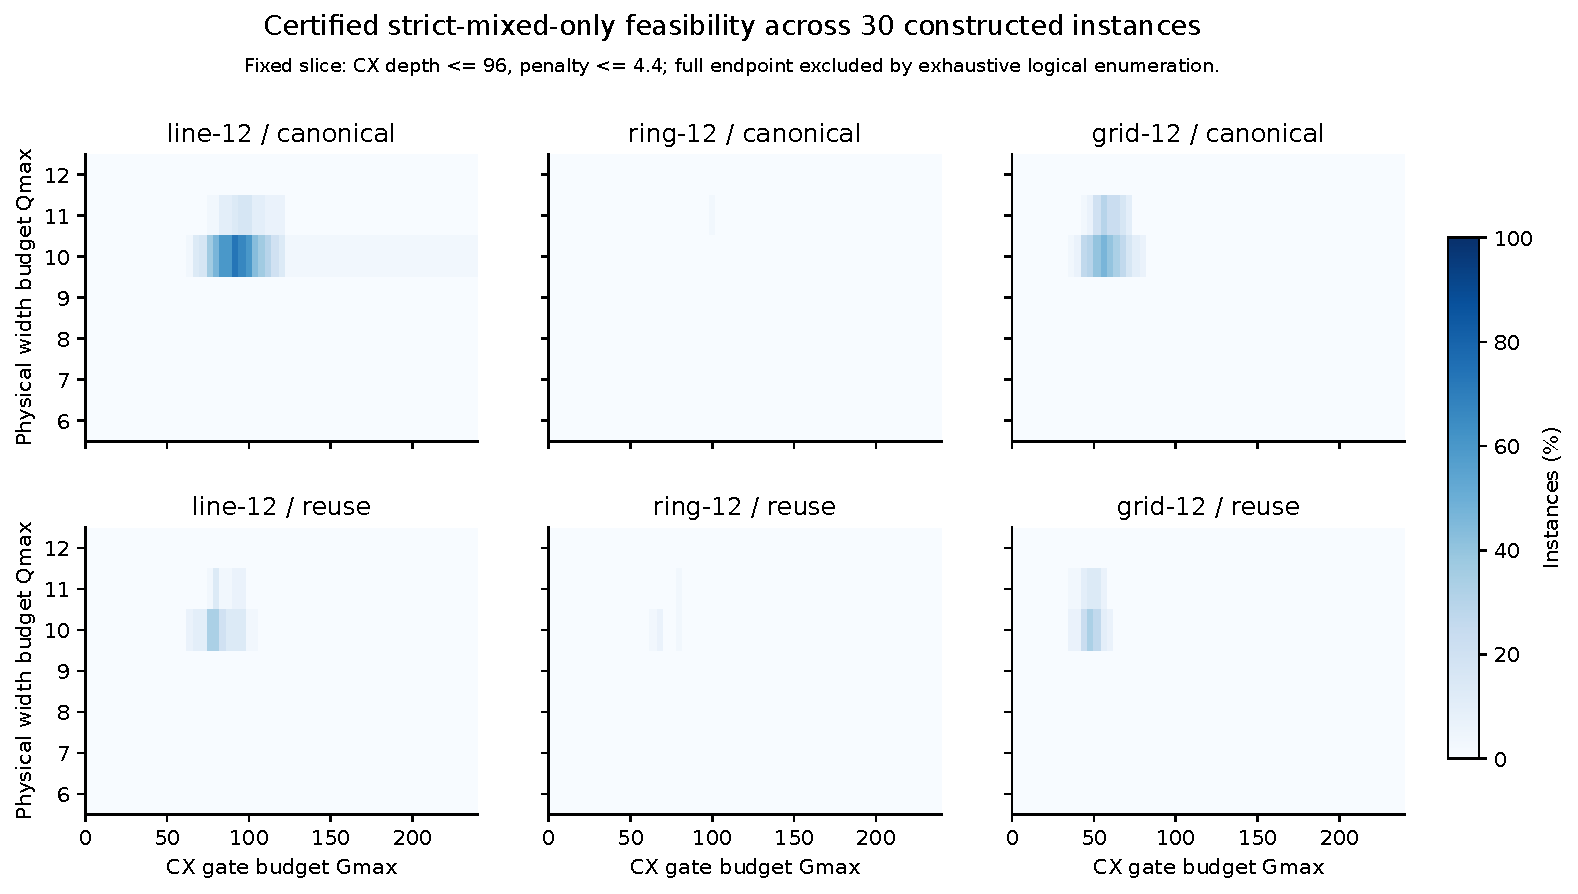
\includegraphics[width=\textwidth]{joint_budget_certified_frequency.pdf}

\caption{Certified mixed-only incidence across the 30 constructed mechanism instances in the fixed $(D_{\max},M_{\max})=(96,4.4)$ slice. Each plotted cell counts independent instances, with the native and full endpoints excluded as specified in Section~\ref{sec:fresh-compiled}. Budget cells and compiler settings are not independent samples.}\label{fig:certified-population}\end{figure}
\FloatBarrier

\subsection{Five-seed delivery and independent checks}
\label{app:multiseed-audit}
The additional data come from
\nolinkurl{URSS_ALL_PROJECT_CODE_20260918T190812Z.zip}, supplied inside
\nolinkurl{delivery.zip}. The inner archive has SHA-256
\seqsplit{54e5629261b6bceb1b8922f7a33aa9f75f87fae5af80f7ccb4ba116349a32014}.
The analysed run is
\nolinkurl{results/multiseed_20260918T163717Z/}.
Earlier incomplete run folders are retained as provenance and are not
pooled with the completed run.

The saved run contains 101,460 completed compiler rows. We independently
recompute all 1,800 budget-classification arrays from these rows.
Every array matches, covering 37,661,400 classified points.
The 5,662-file package manifest and 3,742-file run manifest also match.
Independent enumeration checks one native, one full and one strictly
mixed representation per instance: all 180 pass exactness and unique-lift
checks, with maximum numerical error $1.78\times10^{-15}$.
Six classification tests and ten small regression tests pass.
These checks do not rerun all compilation tasks.
Candidate checks, circuit digests and source hashes provide separate
records of what was run.

The delivered audit records three unresolved output problems. Its
baseline-winner feasibility field was not computed; its YAML file omitted
settings present in the authoritative JSON file; and its region-presence
figure reused one value across seeds. A further check finds that its
``lost or changed'' field counts points lost in every other seed, rather
than points lost in at least one seed. The two counts differ. They cannot
support the same stability label.

We retain the supplied files unchanged and provide a separate correction
script, derived tables and a new figure. The manuscript uses these checked
outputs. The retained-point total, 79,069 out of 149,439, is unchanged.
The original audit failure remains part of the record; the corrected
analysis does not turn the original archive into an unqualified PASS.

The delivery also records two inaccessible source directories and omits
the environment used for the formal Qiskit 2.5.2 run. The copied frozen
inputs and saved results allow the data checks reported here.
They do not establish complete reconstruction of that environment or
coverage of the inaccessible directories. No additional QAOA optimisation
was run for this follow-up.

\section{Additional Experimental Protocol Details}
\label{app:experimental-details}

\subsection{Benchmark definitions and structural coordinates}
\label{sec:applications}

We use weighted Max-3SAT and cubic spin glasses to study how selective
reduction trades interaction locality against auxiliary variables and compiled
resources. Max-3SAT supplies clause-derived signs and overlap; spin glasses
allow sparsity and pair reuse to be varied directly.

\subsubsection{Max-3SAT}

Consider a clause $C=(\ell_i\lor\ell_j\lor\ell_k)$. Define the false-literal indicator
\begin{equation}
    u_{\ell_r}(x_r)
    :=\begin{cases}
       1-x_r, & \ell_r=x_r,\\
       x_r, & \ell_r=\neg x_r.
    \end{cases}
    \label{eq:false-indicator}
\end{equation}
The clause-violation penalty is
\begin{equation}
    P_C(\bm x)=u_{\ell_i}(x_i)u_{\ell_j}(x_j)u_{\ell_k}(x_k),
    \label{eq:clause-penalty}
\end{equation}
which equals one exactly when the clause is violated. A weighted Max-3SAT
instance with $w_C>0$ therefore yields the cubic PUBO~\cite{Nagies2025,Nusslein2023}
\begin{equation}
    f_{\mathrm{3SAT}}(\bm x)=\sum_{C}w_CP_C(\bm x).
    \label{eq:max3sat-pubo}
\end{equation}
After expansion and coefficient aggregation, cubic terms that share a variable
pair can use the same auxiliary. Cancellation must be accounted for before
selecting substitutions and setting penalties; the expansion for arbitrary
literal signs is given in Appendix~\ref{app:max3sat}.

\paragraph{A small worked example}
\label{sec:max3sat-worked-example}

Consider the five-variable weighted instance
\begin{equation}
 f_{\mathrm{3SAT}}^{\mathrm{ex}}(\bm x)
 =g(\bm x)+5x_1x_2x_3-4x_2x_3x_4+2x_1x_4x_5,
 \label{eq:max3sat-worked-expanded}
\end{equation}
where $g(\bm x)=4-4(x_2+x_3+x_4)+4(x_2x_3+x_2x_4+x_3x_4)$.
The clauses and full expansion are given in
Appendix~\ref{app:max3sat-worked}.
The first two cubic terms share $\{2,3\}$. Substituting $y_{23}=x_2x_3$
gives the aggregate residual $A_{23}=5x_1-4x_4$, so
\cref{prop:cubic-mixed-sign} gives the sharp threshold
$M_{23}^{*}=\max\{5,4\}=5$. Taking $M_{23}=6$ yields
\begin{align}
 F_{\mathrm{sel}}(\bm x,y_{23})
 ={}&g(\bm x)+5x_1y_{23}-4y_{23}x_4+2x_1x_4x_5 \nonumber\\
 &+6\PR(x_2,x_3,y_{23}).
 \label{eq:max3sat-worked-selective}
\end{align}
The native representation retains all three cubic terms. Full quadratization
also substitutes $y_{14}=x_1x_4$ in the remaining term, with threshold
$M_{14}^{*}=2$ and penalty $M_{14}=3$. All three representations preserve
the original objective under auxiliary minimisation, as verified in
Appendix~\ref{app:max3sat-worked}.
\Cref{tab:max3sat-worked-comparison} shows the trade-off: the selective choice
removes two cubic terms using one auxiliary, while saving one auxiliary and
four quadratic couplings relative to full reduction. These logical counts do
not establish a compiled-resource or QAOA advantage; those are tested separately.

\begin{table}[t]
    \centering
    \small
    \caption{Logical comparison for the worked Max-3SAT instance. Quadratic
    couplings count distinct degree-two monomials after aggregation.}
    \label{tab:max3sat-worked-comparison}
    \begin{tabular}{@{}lccccc@{}}
        \toprule
        Encoding
        & \shortstack{Total\\variables}
        & \shortstack{Auxiliary\\variables}
        & \shortstack{Retained\\cubic terms}
        & \shortstack{Quadratic\\couplings}
        & Penalties\\
        \midrule
        All-native & $5$ & $0$ & $3$ & $3$  & --\\
        Selective  & $6$ & $1$ & $1$ & $7$  & $M_{23}=6$\\
        Fully quadratized & $7$ & $2$ & $0$ & $11$
            & $M_{23}=6,\ M_{14}=3$\\
        \bottomrule
    \end{tabular}
\end{table}

\subsubsection{Cubic spin glasses}

Higher-order spin-glass models provide a complementary benchmark
\cite{Basso2022,PelofskeShortDepth2024,Pelofske2024}.
For $s_i\in\{-1,+1\}$, write
\begin{equation}
 E(\bm s)=c+\sum_i h_is_i+\sum_{i<j}J_{ij}s_is_j
 +\sum_{i<j<k}K_{ijk}s_is_js_k.
 \label{eq:cubic-spin}
\end{equation}
The main study uses the pure cubic case $c=h_i=J_{ij}=0$.
Substituting $s_i=1-2x_i$ gives a PUBO of degree at most three.
Appendix~\ref{app:spin-glass} specifies the conversion and common rescaling
convention. Varying the cubic supports provides different opportunities for
pair reuse without deriving the interactions from clauses. The two families
are contrasting tests, not a controlled separation of application effects
from hypergraph effects.

\subsubsection{Structural coordinates and benchmark scope}
Analytical QAOA guarantees for regular MaxCut graphs~\cite{Wurtz2021}
and high-depth analyses on large-girth graphs and
hypergraphs~\cite{BassoHighDepth2022} concern specified graph families
and limiting regimes. The finite benchmark ensembles below serve a
different purpose: measuring paired resource and optimisation changes
under exact representation choices.

\label{sec:benchmark-generation}

The main structural axes are cubic sparsity, potential auxiliary reuse, and
hardware connectivity. Coefficient signs affect the penalty through
\cref{eq:cubic-threshold}, but sign balance is recorded as a diagnostic rather
than varied as an additional main axis.

All clauses or hyperedges are expanded and equal monomials are aggregated
before structural features are calculated.  Let $\mathcal C_3(f)$ denote the
remaining nonzero cubic supports and $m_3=|\mathcal C_3(f)|$.  We record the
canonical cubic density $m_3/\binom{n}{3}$ and the load $m_3/n$.  The pair shadow
$\partial_2\mathcal C_3$ is the set of all pairs contained in at least one
cubic support.  Potential pair sharing is summarised by the pair-incidence
score
\begin{equation}
  r_{\mathrm{pair}}
  =1-\frac{|\partial_2\mathcal C_3|}{3m_3},
  \qquad m_3>0,
  \label{eq:pair-reuse-score}
\end{equation}
together with $d(p)=|\{S\in\mathcal C_3(f):p\subseteq S\}|$ and
$\Delta_2=\max_{p\in\partial_2\mathcal C_3}d(p)$.  This score
is zero when every cubic term has three private pairs and increases when pair
incidences are repeated.  It measures potential sharing, not the number of
auxiliaries actually saved by a chosen representation.  When the exact pair
cover is available, the corresponding full-reduction saving is
\begin{equation}
  r_{\mathrm{aux}}
  =1-\frac{\tau_2(\mathcal C_3(f))}{m_3},
  \qquad m_3>0,
  \label{eq:auxiliary-saving-score}
\end{equation}
where $\tau_2$ is the set-cover number defined in \cref{eq:pair-cover}.

Connectivity is assessed by compiling representations of the same instance to
common target graphs. The main targets are all-to-all coupling and a 12-qubit
$3\times4$ grid; additional line, ring, and heavy-hex targets extend the
routing comparison. Capacity failures and common-fit comparisons are handled
by the protocol in Section~\ref{sec:experiments}.

The three workload tiers have different purposes. The oracle tier targets
30 instances per family with $n\in\{5,6,7,8\}$; the QAOA tier targets 36 per
family with $n\in\{6,8,10\}$ and a 12-qubit width limit; the compilation tier
targets 90 per family with $n\in\{8,12,16,20\}$. These generation targets are
distinct from the evaluated subsets reported with each result. The limited
noise subset contains nine instances per family. A separate warm-start study
uses ten instances per family selected using relaxation information only,
without inspecting QAOA outcomes. This strongest-screened set is not pooled
with the original representation comparison. Complete sampling, filtering,
screening, and provenance rules are given in
Appendix~\ref{app:benchmark-generation}.

\subsection{Detailed evaluation protocol}
\label{app:detailed-evaluation-protocol}

We test exactness, compiled resources, and QAOA performance separately. All
comparisons use representations of the same raw instances and a common
execution protocol; full implementation details are given in
Appendices~\ref{app:reproducibility} and~\ref{app:experimental-details}.

\subsubsection{Benchmark scope and comparison rules}
\label{sec:benchmark-tiers}

The oracle tier contains 60 instances for exhaustive exactness and selector
checks, and the compilation tier contains 180 instances for resource
comparisons. The main noiseless QAOA comparison uses 14 test-labelled
instances; the noise and targeted warm-start studies use separate subsets of
18 and 20 instances, respectively. Each set is balanced between the two
families. These evaluated sets are distinct from the generation targets in
Section~\ref{sec:benchmark-generation} and are analysed separately by study.

We compare the native objective, a fully quadratized reference, the selective
design from Section~\ref{sec:selection}, and a matched-random selective
control. Full quadratization uses a minimum-cardinality pair cover with
deterministic tie-breaking. The random control matches only the number of
active pair auxiliaries, not gate count, depth, or penalty size. Five seeded
controls are used; they need not be distinct when the feasible choices are
limited. The exact construction and fallback rules are in
Appendix~\ref{app:experimental-controls}.

Within each family and tier, the recorded training--validation--test split is
$60/20/20$. Settings were chosen using training and validation data, with no
direct selector retuning on test-labelled rows. However, the pool was
available during earlier protocol refinement, so this is an exploratory
study, not a fresh untouched-test evaluation. The broad resource comparison
pools all 180 compilation instances across split labels.

\subsubsection{Exactness and penalty checks}
\label{sec:exactness-protocol}

On each oracle instance we enumerate the original assignments and minimise
over the auxiliary variables, checking
\begin{equation}
 f(\bm x)=\min_{\bm y}F_\rho(\bm x,\bm y)
 \quad\text{for every }\bm x.
 \label{eq:experimental-pointwise-check}
\end{equation}
The main experiments use $M_p=T_p+1$ and check that the minimising auxiliary
assignment is unique and consistent. Tightness checks use $T_p-1$, $T_p$,
and $T_p+1$, recording mismatches, ties, inconsistent minimisers, and explicit
failure witnesses. Penalty-margin sensitivity runs are reported separately.

\subsubsection{Logical and compiled resources}
\label{sec:resource-protocol}

We record register width, auxiliary count, retained cubic terms, aggregated
quadratic couplings, maximum penalty, and coefficient dynamic range. Every
representation uses the same synthesis and compiler settings and the same
five transpiler seeds on all-to-all coupling and the 12-qubit $3\times4$
grid. The compiled metrics are two-qubit gate count, two-qubit depth, and
routing overhead, including inserted SWAPs.

A width failure is recorded separately, not assigned an artificial gate count.
Direct comparisons use instances on which all representations in that
comparison fit the same device. The connectivity extension compares only
selective and matched-random designs on a 12-qubit line, a 12-qubit ring,
and a 19-qubit heavy-hex graph, without rerunning QAOA. Software, coupling
maps, and seeds are specified in Appendix~\ref{app:reproducibility}.

\subsubsection{Relaxation, selection, and warm starts}
\label{sec:experimental-relaxation}

We solve a sparse RLT-style, strengthened recursive-McCormick LP for the
original cubic objective. It uses single, pair, and supported triple
pseudo-moments in $[0,1]$; only the single and pair coordinates are exported
for selection and warm starts. Cubic terms are represented directly in the
LP, without Rosenberg penalties. The complete constraints and solver rules
are given in Appendix~\ref{app:experimental-lp}.

The selector uses the settings in \cref{tab:selector-settings}. In these
experiments, selection and oracle certification use the exact all-to-all
reference synthesis of Appendix~\ref{app:reference-compiler}.
Device-transpiled resources are evaluated subsequently for the selected
representations. Complete
enumeration and branch-and-bound certification are run on the 60 oracle
instances. A separate sensitivity study varies selector settings on that tier,
without rerunning QAOA; details are in Appendix~\ref{app:experimental-sensitivity}.

\begin{table}[t]
\centering
\small
\caption{Main selector settings. The resource order is auxiliary count,
two-qubit gates, two-qubit depth, and maximum penalty. The broader compilation
tier does not impose the 12-qubit QAOA width limit.}
\label{tab:selector-settings}
\begin{tabular}{@{}p{0.39\linewidth}p{0.56\linewidth}@{}}
\toprule
Setting & Value\\
\midrule
Resource weights & $(0.05,0.45,0.45,0.05)$\\
Normalisation scales & $(6,128,96,64)$\\
QAOA-scope limits & 12 qubits; 256 two-qubit gates per cost layer;
 two-qubit depth 192; maximum penalty 128\\
Selector fibre-diagnostic threshold & $0.02$\\
Beam width; main penalty margin & $64$; $1$\\
Warm-start clipping & $\delta=0.05$\\
\bottomrule
\end{tabular}
\end{table}

Warm-start comparisons use cold start, original-only warming, and
original-plus-auxiliary warming with either pair moments or the independence
approximation. The corresponding probabilities and matched mixers follow
Section~\ref{sec:warm-start}; the experimental policies are specified in
Appendix~\ref{app:experimental-warm}.

The original warm-start runs (E4) use the first LP optimum returned by HiGHS.
The selector and targeted warm-start study use a second, deterministic
optimisation to choose one of the LP's optimal solutions. The two rules can
return different pseudo-moments for the same instance. The 20 targeted
instances were screened using relaxation information, before inspecting
QAOA outcomes. They have the strongest screening scores in the candidate
pool and do not form a representative random sample. We analyse them
separately from original E4.
The coordinate correction restores the saved probability vectors and fixed
designs in both studies. It does not solve the LP again or screen new
instances. Appendix~\ref{app:warmstart-correction-provenance} describes the
execution and checks.

\subsubsection{QAOA budgets and optimisation objective}
\label{sec:qaoa-evaluation}

Each representation is optimised independently using COBYLA, with three
restarts and at most 60 objective evaluations per restart. The loss is the
original-objective expectation $\mathcal E_f$, obtained by ignoring the
auxiliary register. Encoded energy and auxiliary consistency are diagnostics,
not terms in this classical loss.

Equal-layer comparisons use $p\in\{1,2\}$. For a two-qubit-gate budget
$B\in\{128,256\}$, let $g_\sigma$ be the median one-layer two-qubit gate
count on the grid over the five transpiler seeds. For $g_\sigma>0$, the
assigned depth is
\begin{equation}
 p_\sigma(B)=\left\lfloor\frac{B}{g_\sigma}\right\rfloor,
 \qquad p_\sigma(B)g_\sigma\leq B.
 \label{eq:qaoa-gate-budget-depth}
\end{equation}
If $g_\sigma>B$, the stored $p=0$ row is an initial-state baseline with no
trainable parameters. In particular, the 128-gate comparison includes such
rows; their counts and the subset on which every design fits at least one
layer are reported separately. The targeted warm-start study uses only
$p=1,2$ and contains no zero-layer rows.

\subsubsection{Aggregation, uncertainty, and supplementary analyses}
\label{sec:structure-noise-protocol}

The raw instance is the statistical unit. For resources, we take the median
over transpiler seeds for each design, then average the five random-control
design values within each instance. For QAOA, we average the three restart
scores per design, then the five random-control design means. No best-seed,
best-restart, or best-random-design selection is used. Paired differences are
formed only after these within-instance aggregations.

Resource comparisons report medians of paired instance differences. QAOA,
warm-start, and noise comparisons report means and two-sided 95\%
Student-$t$ intervals across instances. The corrected warm-start intervals
use $n-1$ degrees of freedom, are unadjusted for multiple comparisons,
and are exploratory; an interval containing zero does not establish
equivalence or absence of an effect. Repeated seeds and restarts are not
additional independent samples. The exploratory regime labels use a separate
within-endpoint stability rule, not population-level confidence intervals;
its thresholds are in Appendix~\ref{app:experimental-statistics}.

Noiseless statevector results are the primary QAOA comparison. The limited
noise study uses 18 structurally selected instances on the grid, with
representative depolarising and readout errors rather than a calibrated real
device. Parameters are optimised noiselessly and reused at both noise levels
without re-optimisation. Full noise, shot, and seed settings remain in
Appendix~\ref{app:reproducibility}. The structural study uses the sparsity,
pair-reuse, and connectivity axes of Section~\ref{sec:benchmark-generation}.
All these analyses are exploratory; intervals describe uncertainty, and
unadjusted multiple-setting $p$-values are not used to claim significance.

This appendix contains the implementation details supporting
Section~\ref{sec:experiments}. Appendix~\ref{app:reproducibility} retains
software versions, compiler configuration, generation records, optimiser
seeds, and noise settings.

\subsection{Fully reduced and matched-random references}
\label{app:experimental-controls}

The historical full-quadratization baseline uses a minimum-cardinality pair cover of all
cubic supports.  Ties are resolved by the lexicographically smallest active
pair set and then by a lexicographic term-to-pair assignment.  This fixes the
auxiliary count and penalty profile rather than leaving ``full'' as an
unspecified quadratization.

The random control matches only the number of active pair auxiliaries.
We generate five feasible controls with seeds
$2026082711$--$2026082715$. First sample a candidate pair set. Then use a
deterministic augmenting-path procedure to assign reduced terms to those
pairs. If 256 pair-set attempts fail, reuse the selected pair set and choose
a random valid assignment. If no distinct control exists, keep the selected
design itself. A native selected design therefore has a native matched
control. Every representation keeps the raw instance identifier, which lets
us compare designs within the same instance.

\subsection{Relaxation and optimum-face selection}
\label{app:experimental-lp}

The implementation records its relaxation as \texttt{SA\_RLT\_level\_2}.
Because conventions for hierarchy levels differ, we define the exact model
used here.  It is a sparse RLT-style~\cite{SheraliAdams1990}, strengthened
recursive-McCormick~\cite{McCormick1976} relaxation of the canonical
cubic objective
\begin{equation}
  f(\bm x)=c_{\varnothing}
  +\sum_i c_i x_i
  +\sum_{i<j}c_{ij}x_ix_j
  +\sum_{i<j<k}c_{ijk}x_ix_jx_k.
  \label{eq:experimental-rlt-canonical}
\end{equation}
Let $\mathcal T:=\{(i,j,k):i<j<k,\ c_{ijk}\neq0\}$.  The LP has one
single-variable pseudo-moment $\widehat\mu_i$ for every original variable, one
pair pseudo-moment $\widehat q_{ij}$ for every $i<j$, and one triple
pseudo-moment $\widehat t_{ijk}$ for every $(i,j,k)\in\mathcal T$.  All are
bounded in $[0,1]$, and the primary objective is
\begin{equation}
  \min_{\widehat\mu,\widehat q,\widehat t}
  \left(
    \sum_i c_i\widehat\mu_i
    +\sum_{i<j}c_{ij}\widehat q_{ij}
    +\sum_{(i,j,k)\in\mathcal T}c_{ijk}\widehat t_{ijk}
  \right).
  \label{eq:experimental-rlt-objective}
\end{equation}
The constant $c_{\varnothing}$ is added back only when the objective value is
reported.  Cubic terms are represented directly by $\widehat t_{ijk}$; no
Rosenberg penalty is used inside this relaxation.

For every $i<j$, the pair envelope is
\begin{equation}
  \widehat q_{ij}\leq\widehat\mu_i,
  \quad
  \widehat q_{ij}\leq\widehat\mu_j,
  \quad
  \widehat q_{ij}\geq\widehat\mu_i+\widehat\mu_j-1.
  \label{eq:experimental-rlt-pair}
\end{equation}
For each $(i,j,k)\in\mathcal T$, the triple variable obeys
\begin{equation}
  \widehat t_{ijk}\leq
  \widehat\mu_i,\widehat\mu_j,\widehat\mu_k,
  \qquad
  \widehat t_{ijk}\geq
  \widehat\mu_i+\widehat\mu_j+\widehat\mu_k-2,
  \label{eq:experimental-rlt-triple-single}
\end{equation}
where the first shorthand denotes three separate upper bounds.  For each
pair--remaining-index decomposition
$(ab,c)\in\{(ij,k),(ik,j),(jk,i)\}$, we additionally impose
\begin{equation}
  \widehat t_{ijk}\leq\widehat q_{ab},
  \qquad
  \widehat t_{ijk}\geq\widehat q_{ab}+\widehat\mu_c-1.
  \label{eq:experimental-rlt-triple-pair}
\end{equation}
These constraints recover the intended products at Boolean points.  At a
fractional solution they are relaxation pseudo-moments and need not be the
marginals of one joint probability distribution.

The LP is solved with SciPy 1.18.1 using
\texttt{scipy.optimize.linprog}, the HiGHS method, and presolve.  The v2
selector uses a second solve after obtaining the primary value $z^\star$.  It
keeps the primary objective within
\begin{equation}
  \left|\bm c^\top\bm v-z^\star\right|\leq10^{-9}
  \label{eq:experimental-rlt-optimum-face}
\end{equation}
and minimises a positive secondary objective whose weights are derived
deterministically from SHA-256 labels.  The variable order is all singles,
lexicographic pairs, and then sorted supported triples.  Under the pinned
solver stack, this supplies the selector with a reproducible representative of
the primary optimum face.  The coordinates $\widehat\mu_i$ and
$\widehat q_{ij}$ are read directly from the returned vector and clipped to
$[0,1]$ only to remove small numerical violations; the triple coordinates are
not exported as selector moments.

E4 uses the same feasible LP and primary objective, but its frozen runs use the
first optimal vector returned by HiGHS rather than the selector's secondary
representative.  Therefore, when the primary optimum face is not a single
point, the selector and E4 can use different pseudo-moment vectors.  Before
interpreting the E4 results, we report the distribution of
$|\widehat\mu_i-1/2|$; instances whose values are almost uniform carry little
warm-start information and are identified as such.

\subsection{Certification and selector sensitivity}
\label{app:experimental-sensitivity}

The main selector settings are listed in \cref{tab:selector-settings}; final
score ties are broken lexicographically.

For the 60 oracle-tier instances, we also ran the best-bound branch-and-bound
procedure of \cref{alg:app-branch-and-bound}.  At each step, the unresolved
state with the smallest valid lower bound is expanded first, and one trace row
is stored after every 256 explored nodes.  A run is declared complete only
when the frontier is resolved, the final lower and upper bounds are equal, and
the selected value matches the previously frozen complete-enumeration optimum.
The compiler contribution in a partial state uses the valid but conservative
lower bound of zero.  These runs therefore check the certificate
implementation on small finite search spaces; they are not a claim about
large-instance scaling.

We performed a one-factor-at-a-time sensitivity study on the same 60 oracle
instances.  Starting from weights $(0.05,0.45,0.45,0.05)$, beam width 64,
fibre threshold 0.02, and penalty margin 1.0, we varied the resource weights,
tested gate-only, depth-only, and joint gate--depth scores, used beam widths
16, 32, and 128, changed the fibre threshold to $0$, $0.01$, $0.05$, and
$0.10$, and changed the penalty margin to $0.5$ and $2.0$.  We also included
a deterministic greedy baseline and a deterministic maximum-pair-reuse
baseline.  This study compares representation choices and resource outputs
only; it does not rerun QAOA.

\subsection{Warm-start policies}
\label{app:experimental-warm}

The warm-start comparison uses clipping value $\delta=0.05$ and compares four policies including cold start. From the relevant LP vector we set
\begin{equation}
  p_i=\operatorname{clip}_\delta(\widehat\mu_i),
  \qquad
  p_{ij}^{\mathrm{pair}}
  =\operatorname{clip}_\delta(\widehat q_{ij}),
  \qquad
  p_{ij}^{\mathrm{ind}}=p_i p_j.
  \label{eq:experimental-warm-probabilities}
\end{equation}
Cold start puts every qubit in $|+\rangle$ and uses the usual $X$ mixer.
Original-only warm start uses $p_i$ and its matched mixer on the original
qubits, while each auxiliary remains at probability $1/2$ with an $X$ mixer.
The original-plus-auxiliary policy also applies a matched mixer to the
auxiliaries, using $p_{ij}^{\mathrm{pair}}$ as the main rule.  The product of
the individually clipped probabilities, $p_{ij}^{\mathrm{ind}}$, is the single
auxiliary ablation, without further clipping. The LP supplies pair coordinates
in these experiments, so this ablation deliberately omits available pair
information.

\paragraph{Null control at fixed optimiser coordinates.}
The cold single-qubit unitary is $e^{-i\beta X}$. With
$B(\omega)=2\sqrt{\omega(1-\omega)}X+(1-2\omega)Z=-h_M(\omega)$,
the implemented warm gate is $e^{-i\beta B(\omega)}$ on every warmed
qubit. Setting \emph{all} original and auxiliary probabilities to $1/2$
therefore gives the same statevector, probabilities, and metrics as cold
start at each parameter vector. The regression covers $p=1,2$, native and
auxiliary designs, and all four policy paths. Setting only the original
probabilities to $1/2$ is insufficient: the independence rule would set an
auxiliary probability to $1/4$. The control explicitly overrides the full
register after policy construction.

\paragraph{Targeted warm-start addendum.}
The 20 strongest-screened instances are evaluated at equal layer depths
$p=1$ and $p=2$.  Every selected representation has at least one active
auxiliary, and no zero-layer bookkeeping row is included.  We compare cold
start, original-variable-only warm start, original-and-auxiliary warm start
using the pair pseudo-moments, and the independence closure
$p_{ij}=p_i p_j$.  Each setting uses three COBYLA restarts and 60 objective
evaluations per restart, giving 480 run rows in total.  All runs use noiseless
statevector evaluation. The archived addendum probabilities were obtained
with the deterministic secondary optimum-face selection used by the v2
selector, whereas the original E4 probabilities came from the first primary
optimum. The correction restores both archived probability sets and reruns
all 480 targeted tasks; it does not invoke either LP selection procedure.

\subsection{Secondary statistics and regime labels}
\label{app:experimental-statistics}

For paired instance differences $d_i$, let $\bar d$ denote their mean.
A paired standardised effect is reported as
$d_z=\bar d/s_d$, where $s_d$ is the sample standard deviation of the paired
instance differences.  Win/tie/loss counts use the same raw instances and the
declared equivalence band.  The E5 endpoint classification retains its frozen
paired normal interval over repeated observations within each endpoint and is used only for the
exploratory regime counts.  The regime study uses frozen
equivalence bands of 5\% for gate count, depth, and routing overhead, and 0.01
objective units for the QAOA score.  A result is called helpful or detrimental
only when its paired interval lies beyond the corresponding band; otherwise it
is assigned to the residual (inconclusive) category. This category includes
intervals overlapping the band and does not establish practical equivalence.

These endpoint intervals describe algorithmic stability, not across-instance
uncertainty. Sign balance and coefficient heterogeneity remain diagnostics,
not additional factorial axes.

\FloatBarrier

\clearpage
\setcounter{section}{0}\setcounter{subsection}{0}
\setcounter{equation}{0}\setcounter{figure}{0}\setcounter{table}{0}
\setcounter{algorithm}{0}
\renewcommand{\thesection}{S\arabic{section}}
\renewcommand{\theequation}{S\arabic{equation}}
\renewcommand{\thefigure}{S\arabic{figure}}
\renewcommand{\thetable}{S\arabic{table}}
\renewcommand{\thealgorithm}{S\arabic{algorithm}}
\renewcommand{\figurename}{Supplementary Figure}
\renewcommand{\tablename}{Supplementary Table}
\renewcommand{\theHsection}{supp.\arabic{section}}
\renewcommand{\theHequation}{supp.\arabic{equation}}
\renewcommand{\theHfigure}{supp.\arabic{figure}}
\renewcommand{\theHtable}{supp.\arabic{table}}
\renewcommand{\theHalgorithm}{supp.\arabic{algorithm}}
\begin{center}\Large\bfseries Supplementary Information\end{center}
\section{Historical development studies}\label{supp:historical}
The earlier studies use 60 oracle instances, 180 compilation instances and
14 noiseless QAOA instances. Each set is balanced between the two families.
They compare native, full, selective and random representations.
The old random controls match only auxiliary count.

QAOA is scored on the original objective after ignoring auxiliary bits.
We form resource differences within each instance.
Instances, not restarts, are the independent units for QAOA intervals.
We analyse the families separately because their objective scales differ.
These are exploratory studies.
Methods (Section~\ref{sec:experiments}) and
Appendix~\ref{app:supplementary-results} give their protocols.

\subsection{Development evidence: exactness and selector validation}
\label{sec:results-exactness}
\label{sec:results-selector-validation}

We check every original assignment and minimise over every auxiliary
assignment in the small oracle cases. Above the penalty threshold,
the reduced minimum equals the original value. The minimising auxiliaries
are unique and correct. At the threshold, an incorrect assignment can tie,
but the minimum value remains correct. Below the threshold, we find
explicit failures. These checks illustrate the distinction between
value exactness and unique correct auxiliaries in
\cref{prop:cubic-mixed-sign}.
Appendix~\ref{app:results-exactness} gives the counts.

The old v2 Pareto beam obeys its raw-moment guardrail on all 60 instances.
It finds the enumerated optimum in 58 cases: all 30 spin cases and
28 of 30 Max-3SAT cases. Its largest score regret is $0.010156$
(\cref{tab:selector-oracle-validation,fig:selector-oracle-summary}).
Both misses have training labels. All 12 test-labelled cases match.
The greedy baseline matches the 30 spin optima, which are native.
It matches no Max-3SAT optimum.

This validates a small historical search space with a diagnostic constraint.
It does not certify the new resource-only selector or the new device-specific
searches.

\begin{table}[!htbp]
\centering
\small
\caption{Oracle-tier validation on 60 instances. Regret is the selector
score minus the enumerated optimum. Certification is a separate exact run;
work and timing details are in Supplementary Section~\ref{app:results-selector}.}
\label{tab:selector-oracle-validation}
\begin{tabular}{@{}lrrr@{}}
\toprule
Method & Zero-regret cases & Mean regret & Maximum regret\\
\midrule
Complete enumeration & 60/60 & 0 & 0\\
Pareto beam & 58/60 & $2.3003\times10^{-4}$ & 0.010156\\
Greedy native-completion & 30/60 & 0.019371 & 0.107292\\
Branch-and-bound certification & 60/60 & 0 & 0\\
\bottomrule
\end{tabular}

\end{table}

Separate branch-and-bound runs find the enumerated optimum on all 60 cases.
Their final gaps are zero. The lower bounds never decrease, and the upper
bounds never increase. Capacity pruning is used in 26 runs.
The conservative resource bound is used in none.
This validates the completed small-instance certificates. It does not show
that branch and bound is faster than enumeration or scales to large cases
(\cref{tab:selector-bnb-certification,fig:selector-bnb-gap}).

These certificates use the declared score, direct-pair search space and fixed
all-to-all compiler. They do not certify optimality on every device.
The implemented guardrail uses frozen floating-point moments and the rule
$\widehat E_{\mathrm{fib}}^{\mathrm{computed}}\leq\tau_{\mathrm{fib}}+10^{-9}$.
The certificate applies to this numerical feasible set. It does not apply
to exact LP moments with zero tolerance.

Changing beam width or penalty margin moderately changes fewer selections
than changing resource weights or the fibre threshold.
In the 48-case calibration ablation, the guardrail removes all 12 recorded
threshold violations. This checks compliance with the guardrail, not its
ability to predict QAOA outcomes.
Supplementary Section~\ref{app:results-selector} gives the sweeps. We do not rerun QAOA for these changes.

\subsection{Development evidence: resource trade-offs}
\label{sec:results-resources}
\label{sec:results-regimes}

Repairing the old selector changes 285 representation/draw groups on
65 fixed compilation instances. We rebuild 7,125 affected resource rows
with the same compiler seeds and topologies. Of these, 2,430 compile and
4,695 are excluded by width as expected. There is no unexpected compiler
failure. The other 23,475 rows keep their archived values and provenance.

All scheduled all-to-all circuits compile. Each family has 90 instances.
For Max-3SAT, selective reduction saves a median of 25 gates and 60.5 depth
units relative to native. For spin glass, it saves 18 depth units but adds
six gates (\cref{tab:e2-all-to-all-paired}). The differences are paired
within instances. This is a gate--depth trade-off, and the outcome depends
on the family.
We pool the split labels for this descriptive comparison.
Appendix~\ref{app:results-resources} gives resource levels and diagnostics.

\begin{table}[!htbp]
    \centering
    \small
    \caption{Median within-instance resource difference from the native
    representation on the all-to-all topology.  Differences are calculated
    after transpiler-seed aggregation, so a negative value means a smaller
    circuit.  The table pools all 90 instances in each family.}
    \label{tab:e2-all-to-all-paired}
    \begin{tabular}{@{}llrr@{}}
        \toprule
        Family & Representation
        & $\Delta$ two-qubit gates & $\Delta$ two-qubit depth\\
        \midrule
        Max-3SAT & Fully reduced  & $-37$ & $-72$\\
                 & Selective      & $-25$ & $-60.5$\\
                 & Matched random & $+4$  & $-15.5$\\
        \addlinespace
        Cubic spin glass & Fully reduced  & $+42$ & $-29$\\
                         & Selective      & $+6$  & $-18$\\
                         & Matched random & $+8.2$ & $0$\\
        \bottomrule
    \end{tabular}
\end{table}

Device width limits change which instances can be compared.
On the 12-qubit grid, 108 native designs fit, but only 57 selective and
21 full designs fit (\cref{tab:e2-sparse-capacity}).
Only 21 instances fit all four representations: 12 Max-3SAT and nine spin
cases. We use these same instances for direct grid comparisons.
This avoids comparing different success-only subsets.

\begin{table}[!htbp]
    \centering
    \small
    \caption{Capacity results on the fixed 12-qubit sparse topology.  The
    counts refer to unique benchmark instances rather than compiler-seed
    rows.}
    \label{tab:e2-sparse-capacity}
    \begin{tabular}{@{}lrr@{}}
        \toprule
        Representation & Feasible instances & Fraction\\
        \midrule
        Native          & 108/180 & 60.0\%\\
        Fully reduced   & 21/180  & 11.7\%\\
        Selective       & 57/180  & 31.7\%\\
        Matched random  & 57/180  & 31.7\%\\
        \bottomrule
    \end{tabular}
\end{table}

\begin{table}[!htbp]
    \centering
    \small
    \caption{Median within-instance difference from native on the 21 instances
    that fit the sparse topology in all four representations.  Differences are
    calculated after seed aggregation; negative values mean lower resource
    use.}
    \label{tab:e2-sparse-common-paired}
    \begin{tabular}{@{}llrrrr@{}}
        \toprule
        Family & Representation
        & $\Delta$ gates & $\Delta$ depth & $\Delta$ SWAP & $\Delta$ routing\\
        \midrule
        Max-3SAT & Fully reduced  & $-16$ & $-29$ & $-3$   & $-5.5$\\
                 & Selective      & $-10$ & $-21$ & $-1.5$ & $-2$\\
                 & Matched random & $+6.5$ & $-3.9$ & $+1.8$ & $+4.8$\\
        \addlinespace
        Cubic spin glass & Fully reduced  & $+45$ & $+13$ & $+7$ & $+22$\\
                         & Selective      & $0$   & $0$   & $0$  & $0$\\
                         & Matched random & $0$   & $0$   & $0$  & $0$\\
        \bottomrule
    \end{tabular}

\end{table}

On the common Max-3SAT subset, selective reduction saves a median of
10 gates and 21 depth units relative to native. Random reduction increases
gate count. The old control fixes auxiliary count, but not reduced-term
count, penalty or pair assignment. The difference therefore does not
isolate the effect of partial reduction.

Eight of nine selective spin designs are native. This explains the zero
selective and random medians. Full reduction increases every listed
resource. Only three common-fit instances have test labels, so these
results are descriptive.
The new controls strengthen the comparison by matching both auxiliary
count and reduced cubic count.

The additional line, ring and heavy-hex tests show the same Max-3SAT pattern
against random reduction. Selective depth is lower on every common-fit
instance. Gate count is lower in every line and ring case and in 54 of
55 heavy-hex cases. Spin medians remain zero.
Heavy-hex has more qubits and fits more instances.
These comparisons therefore mix connectivity and capacity effects
(Appendix~\ref{app:results-connectivity}).

\Cref{fig:e5-regime-map-2d} groups the savings by cubic sparsity and pair reuse.
The supplementary stability screen favours selective over random in
20/20 estimable Max-3SAT depth endpoints and 19/20 gate endpoints.
These endpoints are descriptive summaries, not independent samples.
Some bins are sparse, and width exclusions change the available cases.
We cannot conclude that more pair reuse always gives larger savings.
Appendix~\ref{app:results-regimes} gives all counts.

\begin{figure}[!htbp]
    \centering
    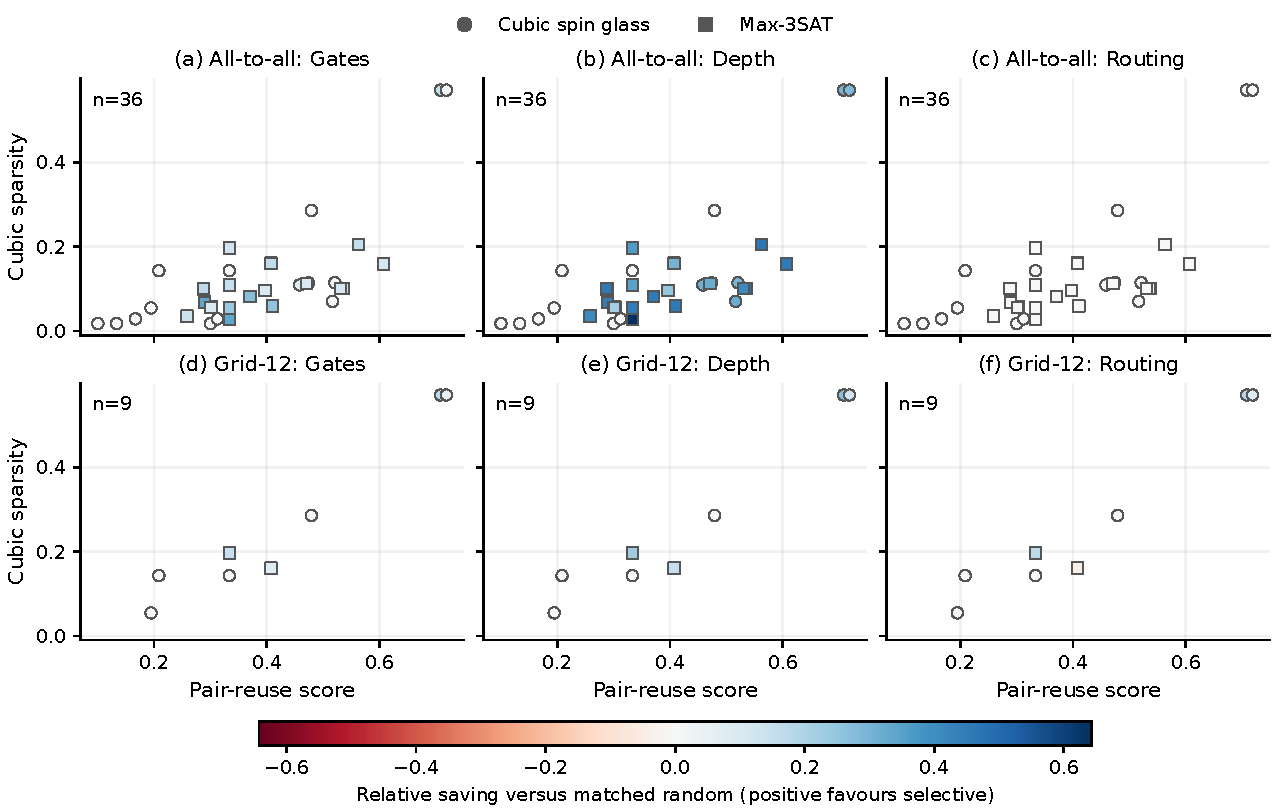
\includegraphics[width=\textwidth]{figure_e5_regime_map_2d.pdf}
    \caption{Two-dimensional representation-regime map from the selector-repaired
    compilation results. Pair reuse and canonical cubic sparsity form the two axes. Panels (a)--(c) show
    all-to-all gates, depth, and routing; (d)--(f) show the same metrics on the
    fixed 12-qubit grid.  Colour is the relative saving of selective reduction over
    its matched-random control, so positive values favour the selective
    design.  Marker shape distinguishes the two benchmark families.}
    \label{fig:e5-regime-map-2d}
\end{figure}

\subsection{Boundary result: native quality under the historical budget}
\label{sec:results-qaoa}

Native has the lowest mean original objective on the 14 development
instances, historically labelled test. This holds in each family at
$p=1,2$ and gate budgets $B=128,256$ (\cref{tab:e3-qaoa-summary}).
In this optimisation protocol, saving circuit resources does not give a
general QAOA-quality improvement.

\begin{table}[!htbp]
    \centering
    \small
    \caption{Mean paired objective difference relative to the native
    representation in the noiseless QAOA study.  Lower is better, so positive
    entries favour the native representation.  Results from the two problem
    families are kept separate because their objective scales differ.}
    \label{tab:e3-qaoa-summary}
    \begin{tabular}{@{}llrrrr@{}}
        \toprule
        Family & Representation
        & $p=1$ & $p=2$
        & $B_{\mathrm{2q}}=128$
        & $B_{\mathrm{2q}}=256$\\
        \midrule
        Cubic spin glass
        & Fully reduced  & 1.837 & 2.041 & 2.044 & 2.458\\
        & Selective      & 0.379 & 0.275 & 0.431 & 0.821\\
        & Matched random & 0.394 & 0.271 & 0.448 & 0.543\\
        \addlinespace
        Max-3SAT
        & Fully reduced  & 1.774 & 2.112 & 0.245 & 1.855\\
        & Selective      & 1.899 & 1.935 & 0.040 & 1.511\\
        & Matched random & 1.390 & 1.192 & 0.385 & 1.516\\
        \bottomrule
    \end{tabular}
\end{table}

Four of the eight selective-minus-native 95\% intervals include zero.
They are the spin cases at $p=1$, $p=2$ and $B=128$, and Max-3SAT at $B=128$.
For Max-3SAT, the difference at $p=2$ is $1.935\;[0.597,3.273]$, favouring
native. At $B=128$ it is $0.040\;[-1.013,1.093]$.
The spin difference at $B=256$ is $0.821\;[0.007,1.635]$.
An interval that includes zero does not prove equal performance.

At the 128-gate budget, 35 of 112 design/draw groups have $p=0$.
These groups account for 105 restart rows. No full cost layer fits, so
these are initial-state baselines with no QAOA optimisation.

If every representation and random draw must fit at least one layer,
only five spin and three Max-3SAT instances remain.
Their selective-minus-native differences are $-0.072\;[-0.544,0.400]$ and
$0.982\;[-0.890,2.854]$, respectively. Both intervals include zero.
\Cref{tab:e3-b128-fit,fig:e3-secondary-metrics} give the breakdown.
The optimised loss is always the original expectation.
Encoded energy and auxiliary inconsistency are separate diagnostics.

\subsection{Exploratory warm-start mechanisms and their limits}
\label{sec:results-warmstart}

The corrected warm-start runs keep the same frozen instances, LP
probabilities and budgets. After selector repair, the audit accounts for
4,176 original E4 rows and 480 targeted rows. It records which zero-layer
rows are reused and which redundant warm policies are removed when a
design has no auxiliaries.
Appendix~\ref{app:warmstart-correction-provenance} gives the records.

The corrected warm mixer uses the cold mixer's angle convention.
This removes a coordinate mismatch in the optimisation comparison.
Warming the original bits and warming the auxiliaries are still separate
changes.

In the original E4 set, 11/14 instances have weak median original-bit bias:
$\operatorname{median}_i|\widehat\mu_i-1/2|\leq0.05$.
This median does not bound every bit's bias or the whole state's distance
from uniformity.

The common selective subset with auxiliaries has only one spin instance
and seven Max-3SAT instances. A spin interval cannot be estimated from
one instance. All four primary Max-3SAT pair-minus-cold intervals include
zero. We keep zero-layer labels at $B=128$
(\cref{tab:e4-warmstart-common,fig:e4-warmstart-corrected}).

\label{sec:results-strong-bias-warmstart}
The targeted study uses 20 strongest-screened instances, ten per family.
Screening uses relaxation information, not QAOA outcomes.
All 480 runs at $p=1,2$ have positive depth.
We analyse this signal-enriched set separately. It does not represent
ordinary random instances.
Its rule for choosing an LP optimum also differs from original E4.
Three selected spin cases still fall below the single-bit signal threshold
(\cref{fig:e4-strong-bias-marginals}).

\begin{table}[!htbp]
\centering\small
\caption{Corrected warm-start results on the 20 strongest-screened instances. We average three restarts, then form paired differences within each instance. Each family has ten instances. Intervals are exploratory 95\% Student-$t$ intervals, without adjustment for multiple comparisons. Negative differences favour the first policy.}
\label{tab:e4-strong-bias-warmstart}
\resizebox{\textwidth}{!}{
\begin{tabular}{@{}llrrr@{}}
\toprule
Family & Depth & Pair minus cold & Pair minus original-only & Pair minus independence\\
\midrule
Spin glass & $p=1$ & $-0.010\;[-0.281,0.260]$ & $-0.116\;[-0.344,0.112]$ & $-0.105\;[-0.320,0.109]$\\
Spin glass & $p=2$ & $0.152\;[-0.026,0.330]$ & $-0.025\;[-0.228,0.179]$ & $0.008\;[-0.289,0.304]$\\
Max-3SAT & $p=1$ & $-6.761\;[-9.263,-4.260]$ & $-0.149\;[-0.219,-0.080]$ & $0.092\;[-0.017,0.202]$\\
Max-3SAT & $p=2$ & $-6.722\;[-9.143,-4.300]$ & $-0.500\;[-0.875,-0.124]$ & $-0.153\;[-0.656,0.350]$\\
\bottomrule
\end{tabular}}
\end{table}

For targeted Max-3SAT, all three warm policies improve on cold start
(\cref{fig:e4-strong-bias-warmstart}). Pair-minus-cold differences are
$-6.761$ at $p=1$ and $-6.722$ at $p=2$. Both intervals are below zero.
Under pair warming, mean optimum probability rises from $0.0360$ to
$0.5987$ at $p=1$, and from $0.0419$ to $0.6262$ at $p=2$.
These probabilities are secondary diagnostics. Spin differences remain
uncertain.

For Max-3SAT, pair-minus-original-only differences are
$-0.149\;[-0.219,-0.080]$ at $p=1$ and
$-0.500\;[-0.875,-0.124]$ at $p=2$.
These exploratory intervals suggest a benefit over warming only the
original bits. They are not adjusted for multiple comparisons.
Both pair-minus-independence intervals include zero.
The study therefore does not establish a stable extra benefit from pair
moments over independence warming.
The limited noise study is separate (Appendix~\ref{sec:results-noise}).

\FloatBarrier

\section{Optional fibre diagnostics: results}\label{supp:v3-diagnostics}
We compare no guardrail, raw-moment filtering and prepared-state filtering.
All use the same mixed candidate bank. The methods, threshold and prediction
model are in main Section~\ref{sec:v3-methods}.

All three rules select the same design on all 72 instances. This is not
because the rules are identical. Of 1,920 random-cohort mixed candidates,
the raw rule rejects 1,243 and the prepared rule rejects 1,329. They disagree
on 86 candidates. All 324 mechanism candidates pass both. In every instance,
the lowest-score candidate passes both rules, so filtering changes no action.
This gives no observed benefit from this intervention. It does not prove
that guardrails always help or never help. Resampling identical zero
differences cannot establish a population-zero effect.

The separate prediction test uses 480 probes chosen in advance from 60 random
instances. To predict an instance, it fits the model using only other
instances. Adding the prepared-state diagnostic lowers inconsistency MSE
from $0.02862839$ to $0.02070590$. The improvement is $0.00792249$, with
descriptive 95\% interval $[0.00376080,0.01273606]$. This is a 27.7\%
relative reduction in held-out MSE. For objective gap, MSE changes from
$0.00148790$ to $0.00139012$. The improvement interval
$[-0.00002862,0.00023108]$ includes zero. Raw diagnostics give a similar
pattern.
These secondary intervals are unadjusted. They resample held-out errors by
instance without refitting the models. The results give limited evidence
that this diagnostic helps predict consistency for the tested model and
instance distribution. They do not establish reliable quality prediction
or show that changing selection causes a gain. The optional threshold rule
still has no demonstrated algorithmic benefit.

\begin{table}[htbp]\centering\small
\caption{Held-out prediction on 480 preselected candidates from 60 random instances. Positive MSE improvement is favourable; intervals are secondary, descriptive and unadjusted.}\label{tab:v3-prediction}
\begin{tabular}{lrrl}\toprule
Outcome & Controls MSE & + Prepared MSE & Improvement [95\% interval]\\\midrule
Quality gap & 0.00148790 & 0.00139012 & $0.00009778\;[-0.00002862,0.00023108]$\\
Inconsistency & 0.02862839 & 0.02070590 & $0.00792249\;[0.00376080,0.01273606]$\\\bottomrule
\end{tabular}\end{table}

\begin{figure}[htbp]\centering
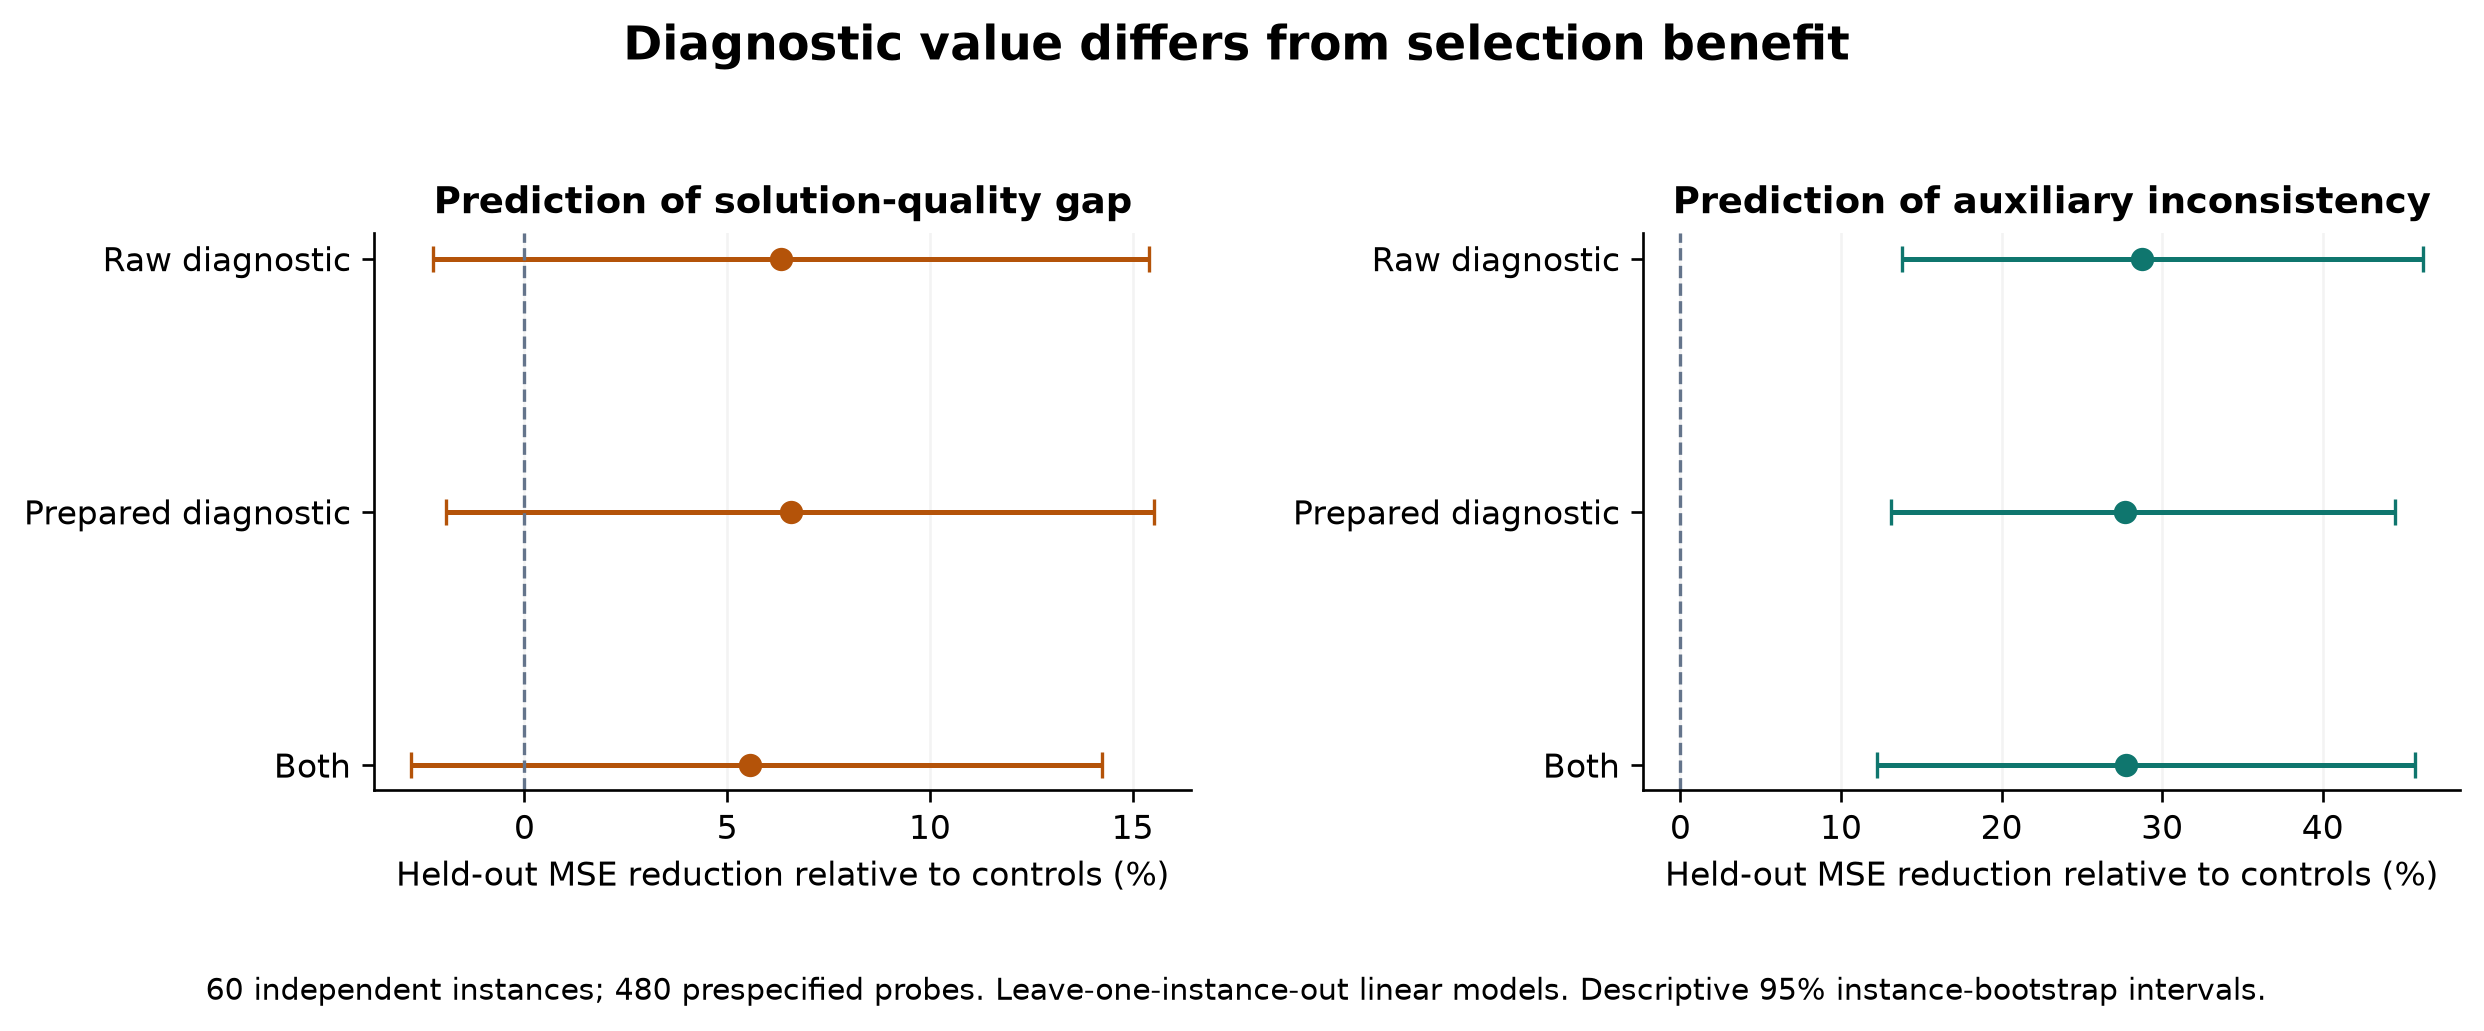
\includegraphics[width=\linewidth]{v3_diagnostic_prediction.png}
\caption{Relative held-out MSE improvement after adding diagnostics to the
control model. Bars are descriptive instance-bootstrap intervals. Prediction gains do not demonstrate selection gains.}\label{fig:v3-prediction}
\end{figure}

\FloatBarrier\section{Additional joint-study display}\label{supp:v3-primary}
\begin{figure}[H]\centering
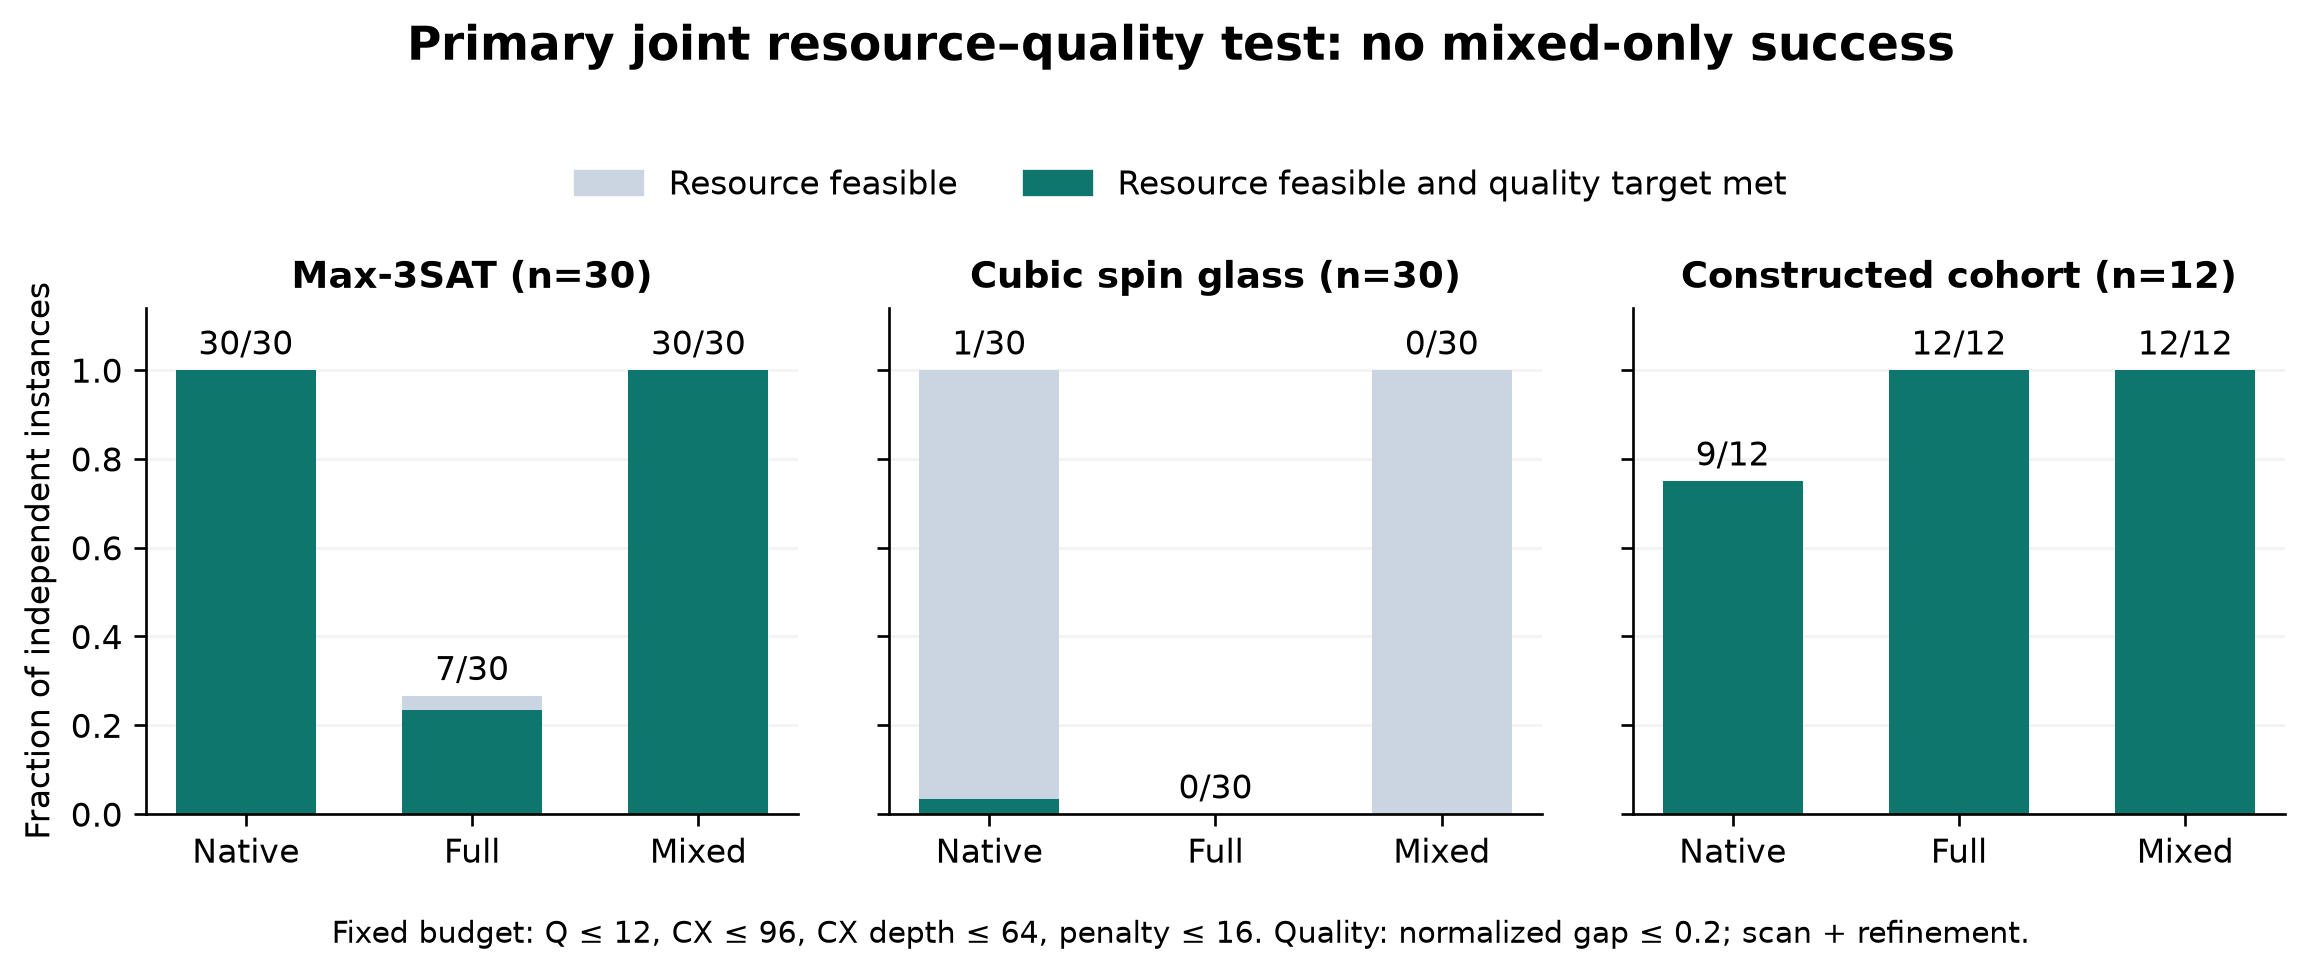
\includegraphics[width=\linewidth]{v3_primary_joint_results.png}
\caption{Primary joint-feasibility outcomes. Grey bars show resource
availability and green bars joint resource-and-quality success. The three cohorts are displayed separately. The main text reports the zero primary mixed-only result.}\label{fig:v3-primary}
\end{figure}

\section{Supplementary Numerical Results}
\label{app:supplementary-results}

These results supplement the four comparisons in Section~\ref{sec:results}.
Protocols and within-instance aggregation follow Section~\ref{sec:experiments}
and Appendices~\ref{app:reproducibility}--\ref{app:experimental-details}.

\FloatBarrier
\subsection{Complete exactness counts}
\label{app:results-exactness}

We first checked the reduction by exhaustive enumeration on 60 small
instances, with 30 Max-3SAT instances and 30 cubic spin-glass instances.  The
selected designs were not all the same: 30 were all-native, 23 were strictly
mixed, and seven were fully reduced.  These instances contain 5,696 distinct
instance--original-assignment pairs.  Across 1,384 representation, design,
penalty, and target-pair trials, the verifier repeatedly enumerated the same
assignments where required, giving 124,672 original-assignment evaluations and
585,408 joint original--auxiliary evaluations in total.  These totals measure
the full verification workload rather than the number of distinct original
assignments.

Section~\ref{sec:results-exactness} summarises the threshold behaviour.
Table~\ref{tab:e1-exactness-summary} reports the counts:
5,351 at-threshold inconsistent ties, 5,639 below-threshold mismatches,
and 452 saved failure witnesses, all with non-zero error.

\begin{table}[!htbp]
    \centering
    \small
    \caption{Summary of the exhaustive exactness checks.  The
    above-threshold setting produced no mismatch or inconsistent minimiser in
    any tested case.}
    \label{tab:e1-exactness-summary}
    \begin{tabular}{@{}lrrr@{}}
        \toprule
        Family and representation
        & \shortstack{At-threshold\\ties}
        & \shortstack{Below-threshold\\mismatch}
        & \shortstack{Saved below-threshold\\witnesses}\\
        \midrule
        Cubic spin glass, fully reduced & 970 & 970 & 78\\
        Max-3SAT, fully reduced          & 268 & 268 & 62\\
        Max-3SAT, selective              & 311 & 315 & 52\\
        Max-3SAT, matched random         & 3,802 & 4,086 & 260\\
        \midrule
        Total                            & 5,351 & 5,639 & 452\\
        \bottomrule
    \end{tabular}
\end{table}

\FloatBarrier
\subsection{Selector validation, certification, and sensitivity}
\label{app:results-selector}

\begin{table}[!htbp]
    \centering
    \small
    \caption{Work and runtime for the oracle-tier methods in
    \cref{tab:selector-oracle-validation}. Entries are medians [interquartile
    ranges]; timings describe the machine used in this study.}
    \label{tab:selector-oracle-work}
    \begin{tabular}{@{}lrr@{}}
        \toprule
        Method & Candidate evaluations & Runtime (s)\\
        \midrule
        Complete enumeration & 4096 [1024, 16384] & 1.274 [0.370, 6.112]\\
        Pareto beam & 640 [448, 832] & 0.832 [0.603, 1.158]\\
        Greedy native-completion & 19 [16, 22] & 0.00525 [0.00414, 0.00667]\\
        \bottomrule
    \end{tabular}
\end{table}

\Cref{fig:selector-oracle-summary} gives the graphical counterpart of
\cref{tab:selector-oracle-validation}. Certification timings and stored gap
traces are given in \cref{tab:selector-bnb-certification,fig:selector-bnb-gap}.

\begin{figure}[!htbp]
    \centering
    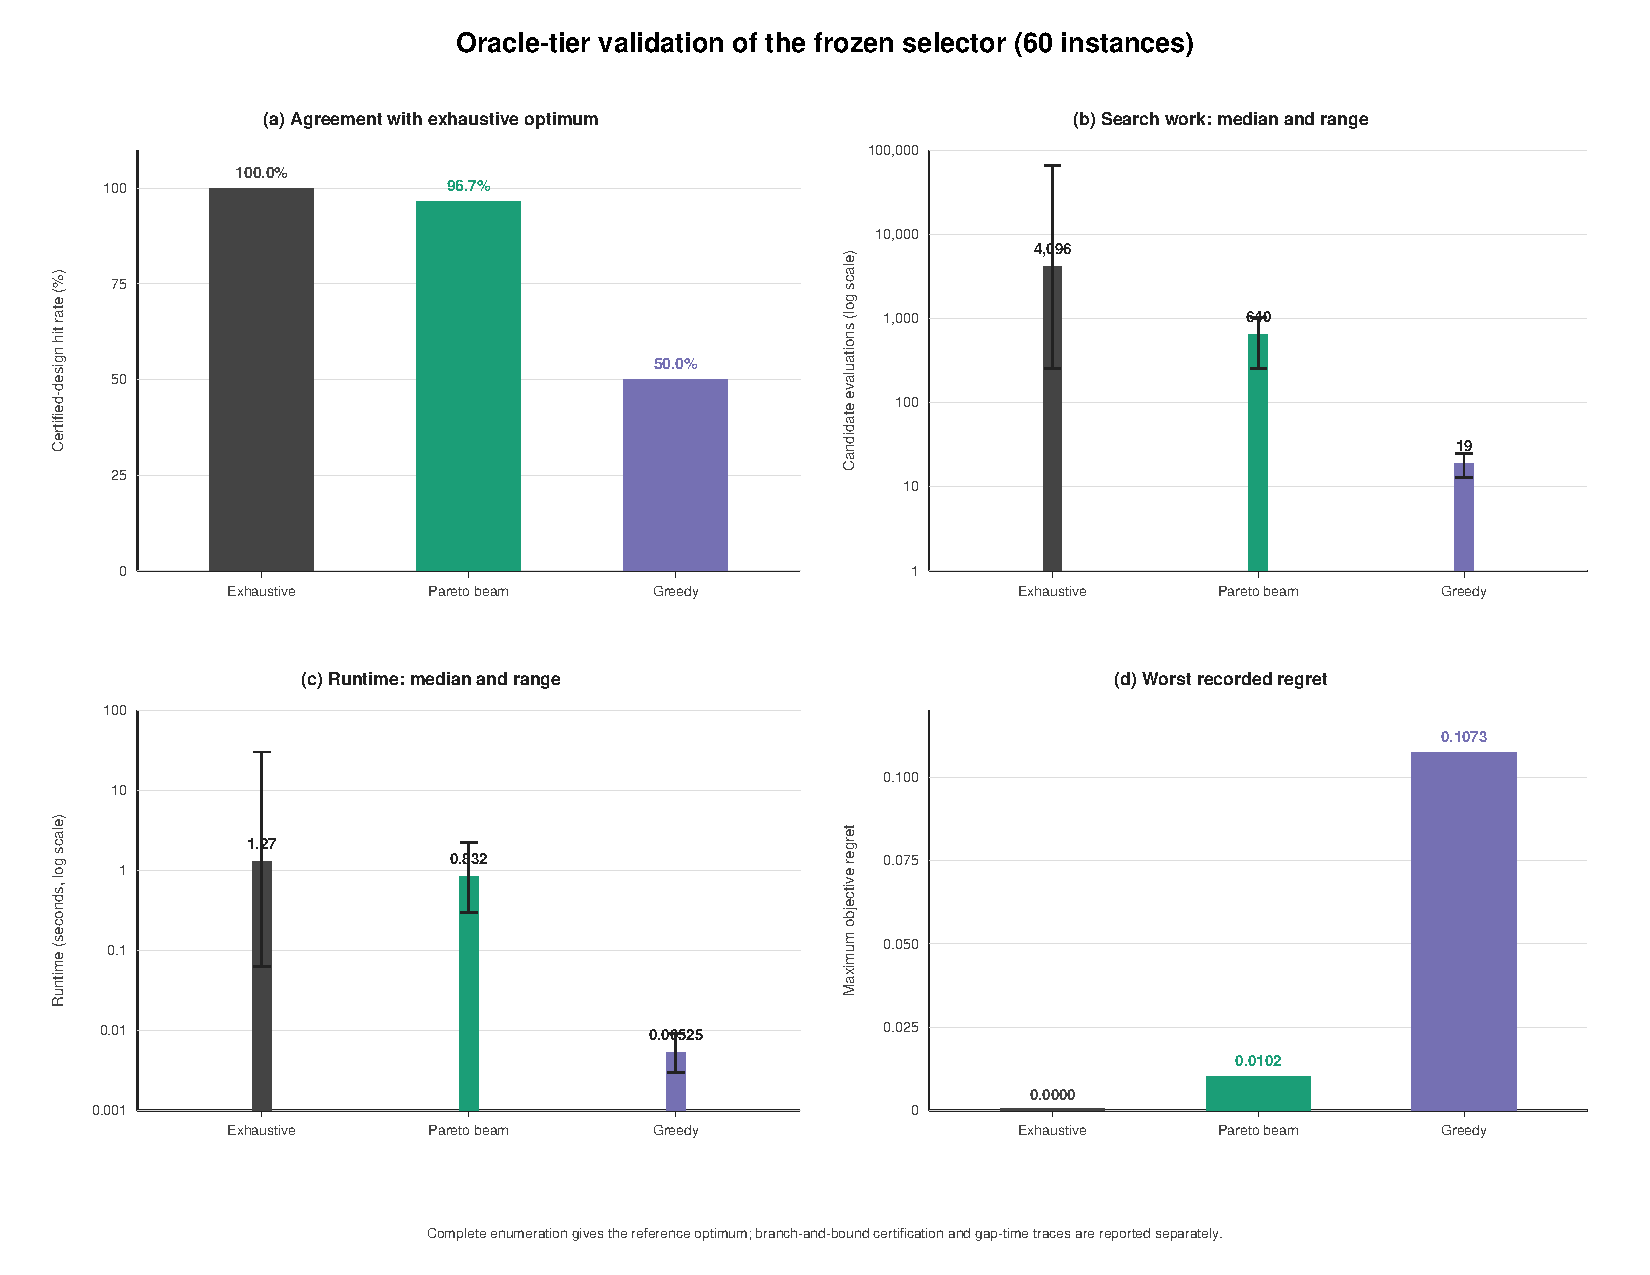
\includegraphics[width=\textwidth]{figure_oracle_selector_summary.pdf}
    \caption{Numerical oracle-tier selector check using the frozen results.
    Complete enumeration supplies the reference optimum, and the practical
    methods are compared with it using hits, work, runtime, and regret.
    Branch-and-bound certification and gap traces are reported separately in
    \cref{tab:selector-bnb-certification,fig:selector-bnb-gap}.}
    \label{fig:selector-oracle-summary}
\end{figure}

\begin{table}[!htbp]
    \centering
    \small
    \caption{Branch-and-bound certification on the oracle tier.  Runtime is
    descriptive for the machine used in this study.}
    \label{tab:selector-bnb-certification}
    \resizebox{\linewidth}{!}{
\begin{tabular}{@{}lrrrrrr@{}}
        \toprule
        Family & Certified
        & Median nodes & Max. nodes
        & Median time (s) & Max. time (s)
        & Max. final gap\\
        \midrule
        Cubic spin glass & 30/30 & 5,461 & 33,462 & 2.469 & 14.715 & 0\\
        Max-3SAT         & 30/30 & 5,461 & 55,453 & 2.336 & 26.526 & 0\\
        \bottomrule
    \end{tabular}}

\end{table}

The repaired certifier can start before any feasible design has been found.
If it stops early, it returns bounds from the remaining search frontier.
The experiments keep the saved floating-point raw moments fixed. A design
passes the fibre check when
$\widehat E_{\mathrm{fib}}^{\mathrm{computed}}\leq\tau_{\mathrm{fib}}+10^{-9}$.
It must also meet the stated resource constraints. Scores and reference
resource bounds use rational arithmetic. The certificate therefore applies
to the feasible set defined by these fixed values and this tolerance.
It does not certify the feasible set based on exact LP moments or the
zero-tolerance definition in Section~\ref{sec:selection}.
All 60 completed historical traces remain valid under the repaired interface.

\begin{figure}[!htbp]
    \centering
    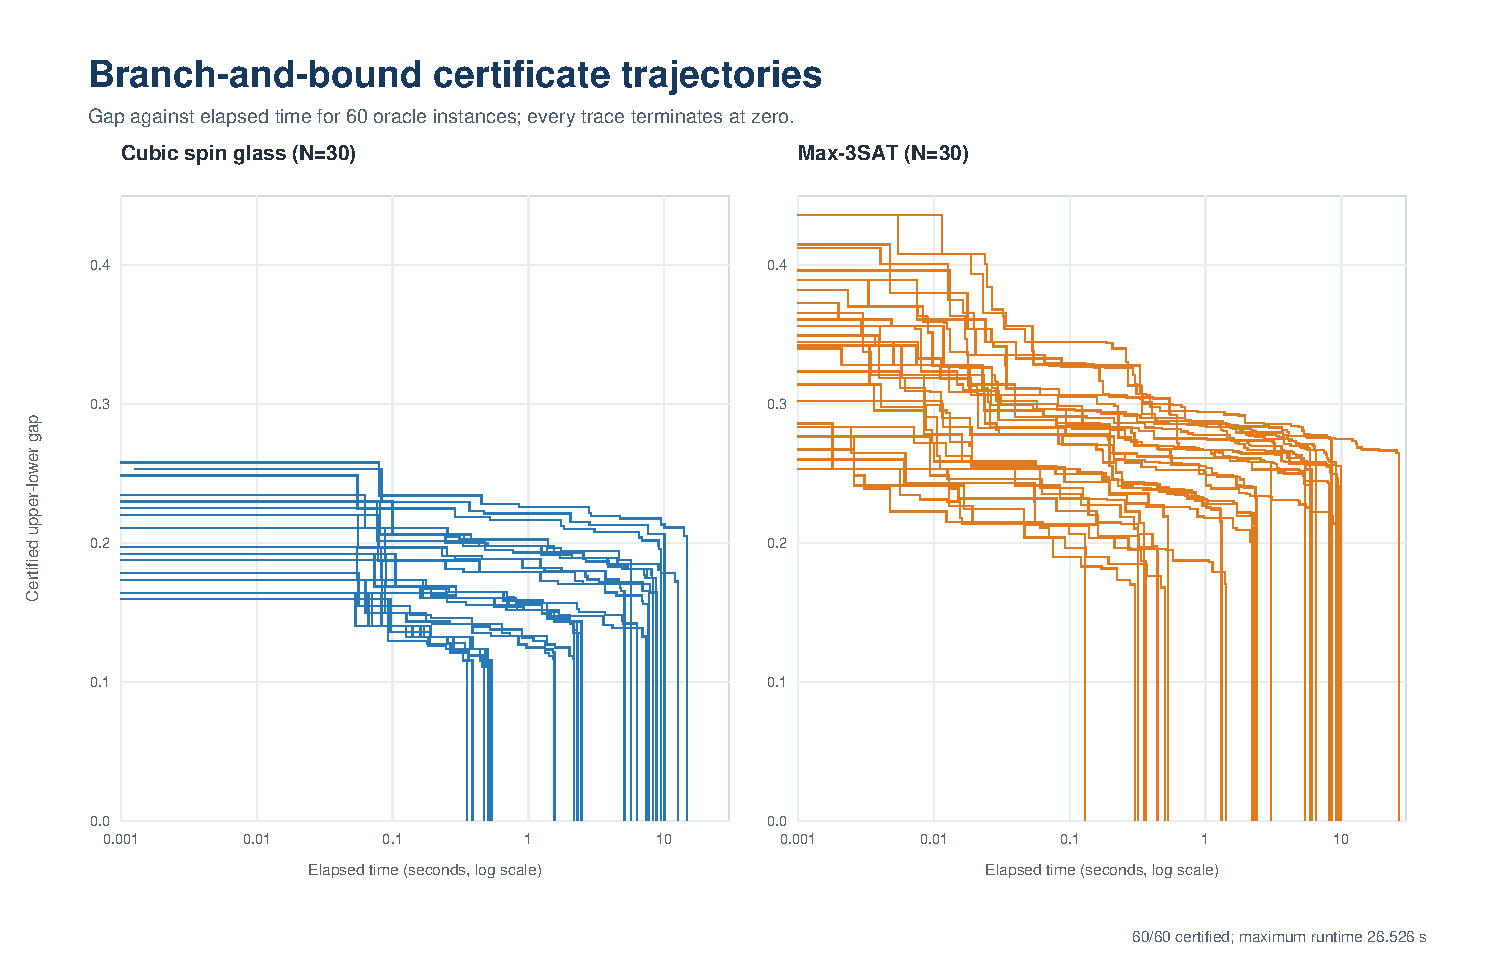
\includegraphics[width=\textwidth]
    {figure_certification_gap_time.pdf}
    \caption{Stored certificate gap against elapsed time for the 60 oracle
    instances: (a) spin glass and (b) Max-3SAT. Each trace terminates at zero.  The figure checks the small
    certification cases and is not used as a scaling claim.}
    \label{fig:selector-bnb-gap}
\end{figure}

\begin{table}[!htbp]
    \centering
    \small
    \caption{Guardrail on/off ablation on the 48 training and validation
    calibration instances.  Fibre-risk medians and score changes use only the
    instances whose selected design changed.  Here
    $\Delta S=S_{\mathrm{guarded}}-S_{\mathrm{unguarded}}$.}
    \label{tab:selector-guardrail-ablation}
    \resizebox{\textwidth}{!}{
    \begin{tabular}{@{}lrrrrrr@{}}
        \toprule
        Split & $n$ & Changed
        & \shortstack{Violations\\off $\rightarrow$ on}
        & \shortstack{Median fibre risk\\off $\rightarrow$ on}
        & Median $\Delta S$ & Max.\ $\Delta S$\\
        \midrule
        Train      & 36 & 10 & $10\rightarrow0$
                   & $0.03142\rightarrow0.01820$ & 0.01654 & 0.03802\\
        Validation & 12 &  2 & $2\rightarrow0$
                   & $0.03301\rightarrow0.01753$ & 0.03451 & 0.04870\\
        Combined   & 48 & 12 & $12\rightarrow0$
                   & $0.03142\rightarrow0.01820$ & 0.01849 & 0.04870\\
        \bottomrule
    \end{tabular}
    }
\end{table}

Without the guardrail, 12 of 48 calibration choices exceeded the threshold.
Enabling it changed exactly these choices and removed all recorded violations,
at a median resource-score increase of $0.01849$ among changed cases. All
changes were in Max-3SAT. This is a training/validation calibration ablation.
The separate one-factor-at-a-time study covers all 60 oracle instances.

\begin{table}[!htbp]
    \centering
    \small
    \caption{One-factor-at-a-time selector sensitivity on 60 oracle
    instances.  ``Changed'' counts representations different from the main
    setting.  Every row uses the same raw instances.}
    \label{tab:selector-sensitivity-addendum}
    \resizebox{\textwidth}{!}{
    \begin{tabular}{@{}llrr@{}}
        \toprule
        Block & Alternative values & Changed choices & Feasible runs\\
        \midrule
        Resource weights
        & equal, auxiliary-heavy, penalty-heavy
        & 30, 30, 27 & 60/60 each\\
        Resource mode
        & gate-only, depth-only, gate--depth
        & 20, 37, 8 & 60/60 each\\
        Beam width
        & 16, 32, 128
        & 5, 2, 1 & 60/60 each\\
        Fibre threshold
        & 0, 0.01, 0.05, 0.10
        & 27, 23, 17, 18 & 60/60 each\\
        Penalty margin
        & 0.5, 2.0
        & 5, 7 & 60/60 each\\
        Greedy baseline
        & deterministic
        & 30 & 60/60\\
        Maximum-reuse baseline
        & deterministic
        & -- & 10/60\\
        \bottomrule
    \end{tabular}
    }
\end{table}

\begin{figure}[!htbp]
    \centering
    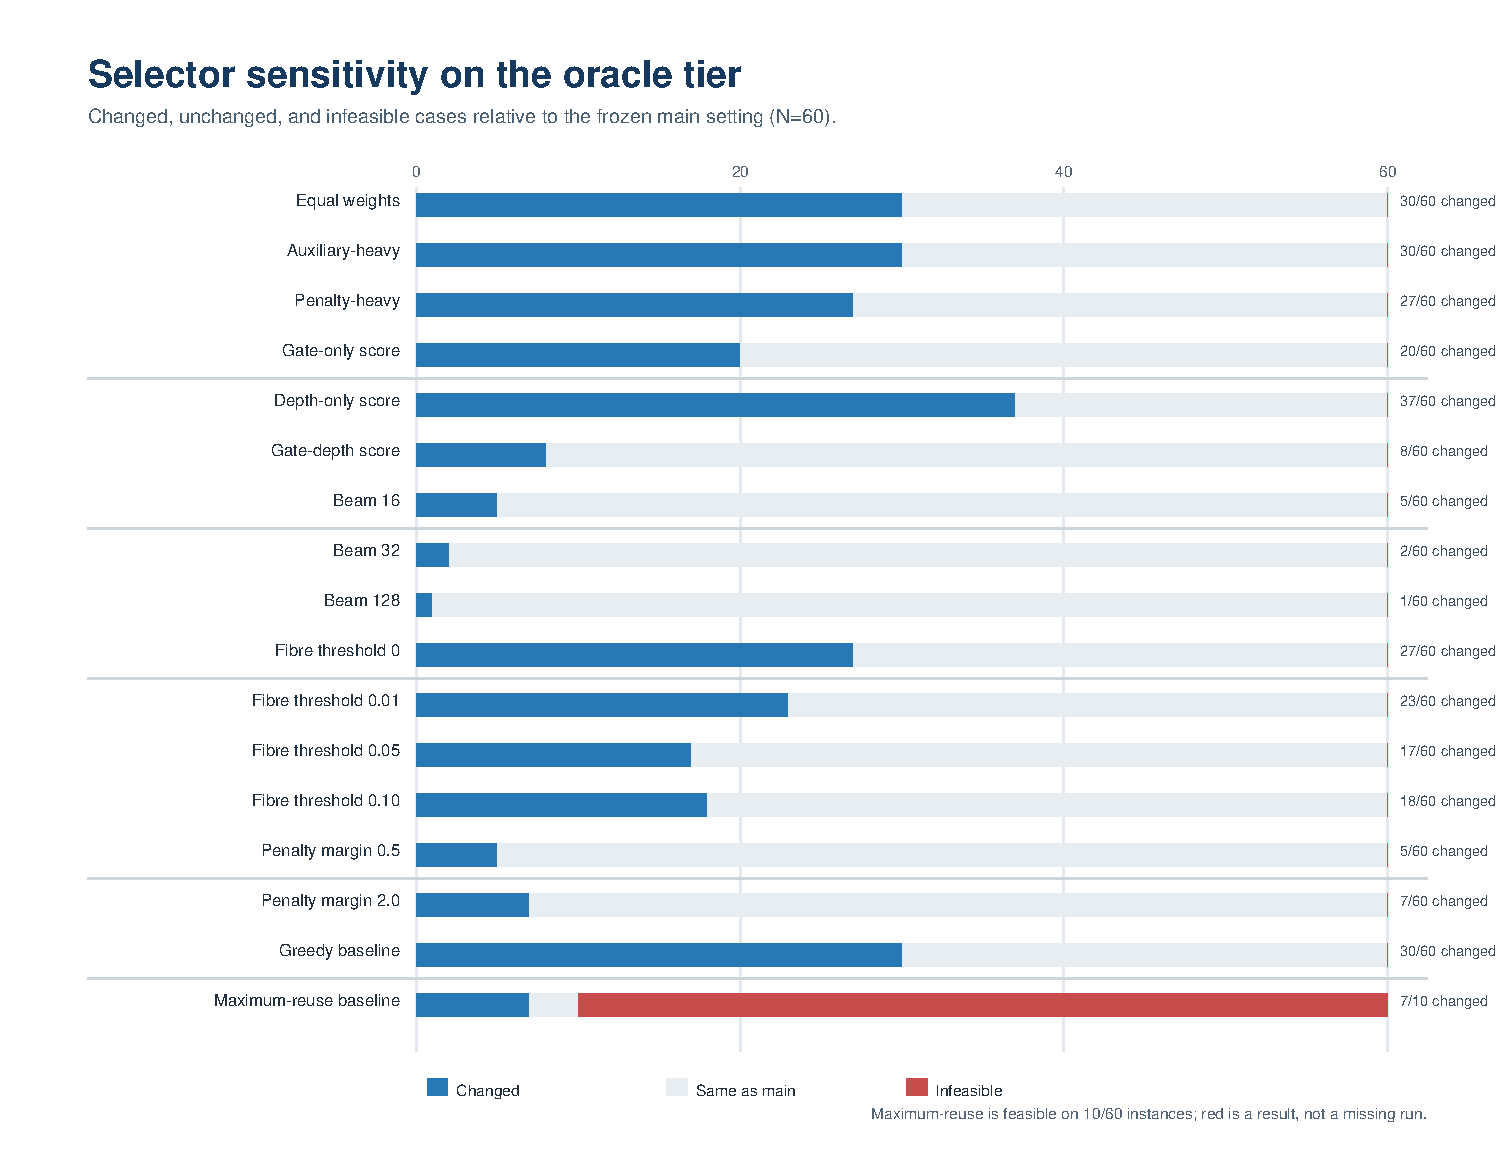
\includegraphics[width=\textwidth]
    {figure_selector_sensitivity_addendum.pdf}
    \caption{Choice stability and feasibility in the selector sensitivity
    study.  A changed choice differs from the frozen main setting.  Red bars
    identify infeasible cases rather than missing runs.}
    \label{fig:selector-sensitivity-addendum}
\end{figure}
The deterministic greedy baseline was feasible in all 60 cases but differed
from the main selector in 30.  The maximum-reuse rule was feasible on only ten
Max-3SAT instances and on none of the spin-glass instances, so it is not a
generally usable replacement for the constrained selector.

Changing the weights changes what the resource score measures. We therefore
do not compare score values directly between weight settings. We use this
test to see whether the selected design changes and to compare its gate
count, depth, auxiliary count and penalty. It does not identify one weight
choice that is best for every problem.

\subsection{Marginal resource levels and selector diagnostics}
\label{app:results-resources}

The all-to-all tier contains 108 training, 36 validation, and 36 test-labelled
instances. Marginal medians describe resource scale; their differences are
not paired effects. For example, selective and native Max-3SAT gate medians
are 145 and 178, while the median paired difference is $-25$, not $-33$.
On the grid, 4,845 of 7,200 scheduled rows are expected width failures, with
no unexpected compiler failures. Main common-fit results are in
\cref{tab:e2-sparse-common-paired}.

\begin{table}[!htbp]
    \centering
    \small
    \caption{Marginal median logical and compiled resource levels on the
    all-to-all reference topology.  These levels show scale, but the difference
    between two entries is not the within-instance paired effect.}
    \label{tab:e2-all-to-all-resources}
    \begin{tabular}{@{}llrrrr@{}}
        \toprule
        Family & Representation
        & Qubits
        & Auxiliaries
        & \shortstack{Two-qubit\\gates}
        & \shortstack{Two-qubit\\depth}\\
        \midrule
        Max-3SAT & Native          & 12 & 0 & 178 & 119.5\\
                 & Fully reduced   & 18 & 7 & 137 & 46\\
                 & Selective       & 18 & 4 & 145 & 56\\
                 & Matched random  & 18 & 4 & 180 & 94\\
        \addlinespace
        Cubic spin glass & Native         & 12 & 0 & 96  & 79\\
                         & Fully reduced  & 18 & 6 & 148 & 47\\
                         & Selective      & 14 & 1 & 116 & 63.5\\
                         & Matched random & 14 & 1 & 117 & 82\\
        \bottomrule
    \end{tabular}
\end{table}

\begin{table}[!htbp]
    \centering
    \small
    \caption{Median diagnostics for the 90 compilation-tier selective designs
    in each family.  Fibre risk is the normalised raw-moment excess used by the v2
    selector guardrail; the threshold is 0.02.  Time is selector runtime in seconds.}
    \label{tab:e2-selector-diagnostics}
    \resizebox{\textwidth}{!}{
    \begin{tabular}{@{}lrrrrrrr@{}}
        \toprule
        Family & Retained cubic & $M_{\max}$ & Dynamic range & Fibre risk
        & Score & Compiler calls & Time\\
        \midrule
        Cubic spin glass & 19 & 9  & 5.5 & 0.00115 & 0.7233 & 4096 & 2.19\\
        Max-3SAT         & 6.5 & 12 & 59.5 & 0.01925 & 0.8156 & 4288 & 1.94\\
        \bottomrule
    \end{tabular}
    }

\end{table}
All 180 compilation-tier selected designs satisfied the raw-moment 0.02
selector guardrail; the
largest stored normalised excess was below 0.02.  The different median retained
cubic counts also show that the repaired v2 selector did not apply the same amount
of reduction to the two families.

We do not report a compilation-tier
certificate gap because these rows are beam-search incumbents and no common
certified lower bound was produced.

\FloatBarrier
\subsection{Additional coupling maps}
\label{app:results-connectivity}

Of 16,200 added compiler rows, 7,020 succeeded and 9,180 were expected width
failures; no unexpected compiler failure was recorded. The table reports
paired medians, while the figure reports means and instance-level intervals.

\begin{table}[!htbp]
    \centering
    \small
    \caption{Selective-minus-matched-random resource differences on the three
    added coupling maps.  Values are paired medians after taking the median
    over transpiler seeds and the mean over matched-random designs within each
    instance.  Negative values favour the selective choice.  Parentheses give
    the number of instances on which selective is strictly lower.}
    \label{tab:e2-additional-topologies}
    \resizebox{\textwidth}{!}{
    \begin{tabular}{@{}llrrrr@{}}
        \toprule
        Topology & Family & Common $N$
        & $\Delta$ two-qubit gates & $\Delta$ two-qubit depth
        & $\Delta$ routing\\
        \midrule
        Line-12
        & Spin glass & 39 & $0.00$ (8) & $0.00$ (9) & $0.00$ (8)\\
        & Max-3SAT   & 18 & $-38.4$ (18) & $-33.3$ (18) & $-26.0$ (18)\\
        Ring-12
        & Spin glass & 39 & $0.00$ (8) & $0.00$ (9) & $0.00$ (8)\\
        & Max-3SAT   & 18 & $-36.3$ (18) & $-31.8$ (18) & $-26.6$ (18)\\
        Heavy-hex-19
        & Spin glass & 65 & $0.00$ (24) & $0.00$ (26) & $0.00$ (24)\\
        & Max-3SAT   & 55 & $-55.8$ (53) & $-52.4$ (55) & $-35.6$ (52)\\
        \bottomrule
    \end{tabular}
    }
\end{table}

\begin{figure}[!htbp]
    \centering
    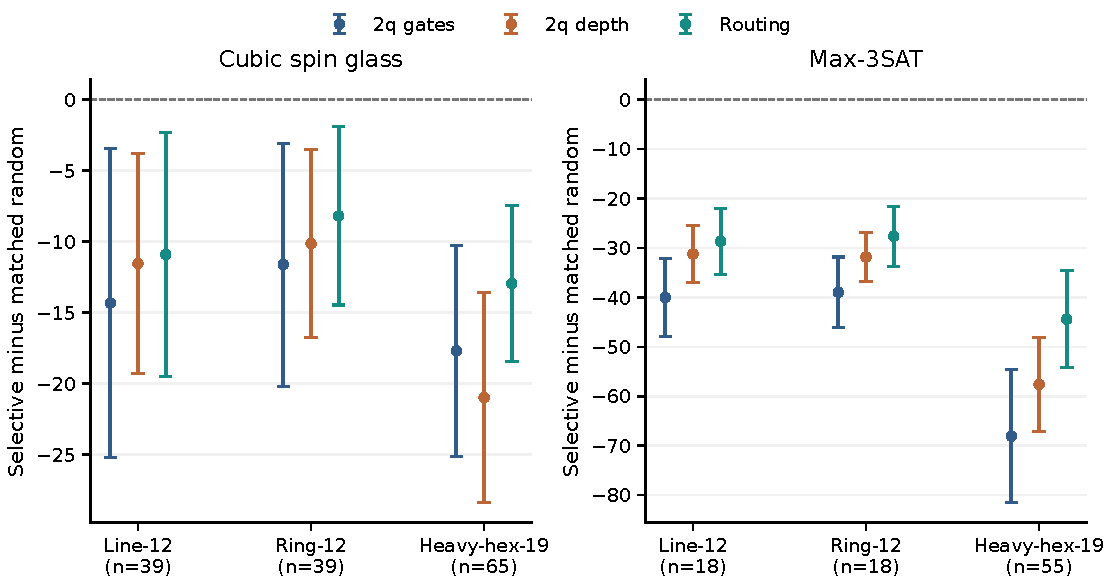
\includegraphics[width=\textwidth]
    {figure_additional_topologies.pdf}
    \caption{Mean paired selective-minus-matched-random resource changes on
    the additional coupling maps: (a) spin glass and (b) Max-3SAT, with 95\% Student-$t$ intervals across raw
    instances.  The comparison uses only instances that fit in both
    representations.  Negative values favour selective reduction; the primary
    medians are reported in \cref{tab:e2-additional-topologies}.}
    \label{fig:e2-additional-topologies}
\end{figure}
Capacity remains part of the result.  The 12-qubit line and ring each had 39
common-fit spin-glass and 18 common-fit Max-3SAT instances, while the
19-qubit heavy-hex graph had 65 and 55.  The corresponding test-labelled
counts were only 7 and 2 on line and ring, and 12 and 9 on heavy-hex.  Since
heavy-hex also has greater capacity, its numerical differences cannot be
attributed to connectivity alone.  The pooled results broaden the
connectivity check, but they remain exploratory rather than a universal
hardware rule.

\FloatBarrier
\subsection{Zero-layer accounting and secondary QAOA diagnostics}
\label{app:results-qaoa}

\Cref{tab:e3-b128-fit} separates the initial-state baselines from designs
that fit at least one layer. Matched-random groups count five draws per raw
instance, and each group contains three restart rows.

\begin{table}[!htbp]
    \centering
    \small
    \caption{Separation of the stored zero-layer baselines at
    $B_{\mathrm{2q}}=128$.  A design/draw group contains three restart rows.
    Matched random has five frozen draws per raw instance.  ``Fully normal''
    means that all draws for the representation have $p\geq1$.}
    \label{tab:e3-b128-fit}
    \begin{tabular}{@{}llrrrr@{}}
        \toprule
        Family & Representation
        & $p=0$ groups
        & $p=0$ rows
        & \shortstack{Instances with\\any $p=0$}
        & \shortstack{Fully normal\\instances}\\
        \midrule
        Spin glass & Native         & $0/7$   & 0  & $0/7$ & $7/7$\\
                   & Full           & $2/7$   & 6  & $2/7$ & $5/7$\\
                   & Selective      & $1/7$   & 3  & $1/7$ & $6/7$\\
                   & Matched random & $5/35$ & 15 & $1/7$ & $6/7$\\
        \addlinespace
        Max-3SAT  & Native         & $4/7$   & 12 & $4/7$ & $3/7$\\
                   & Full           & $2/7$   & 6  & $2/7$ & $5/7$\\
                   & Selective      & $2/7$   & 6  & $2/7$ & $5/7$\\
                   & Matched random & $19/35$ & 57 & $4/7$ & $3/7$\\
        \bottomrule
    \end{tabular}
\end{table}
Requiring every representation and all five matched-random draws to fit at
least one layer leaves only five spin-glass and three Max-3SAT instances.  On
this strict common subset, the spin-glass selective and matched-random paired
objective differences from native are $-0.072$ $[-0.544,0.400]$ and $-0.183$
$[-0.981,0.615]$, respectively.  Both intervals include zero.  For Max-3SAT,
the corresponding means are 0.982 $[-0.890,2.854]$ and 0.941
$[0.603,1.280]$.  This small common-fit analysis is exploratory.  Overall, the
experiment does not show a general QAOA performance benefit from selective
reduction; it shows that a resource saving does not automatically lead to a
better finite-depth objective value.

\begin{figure}[!htbp]
    \centering
    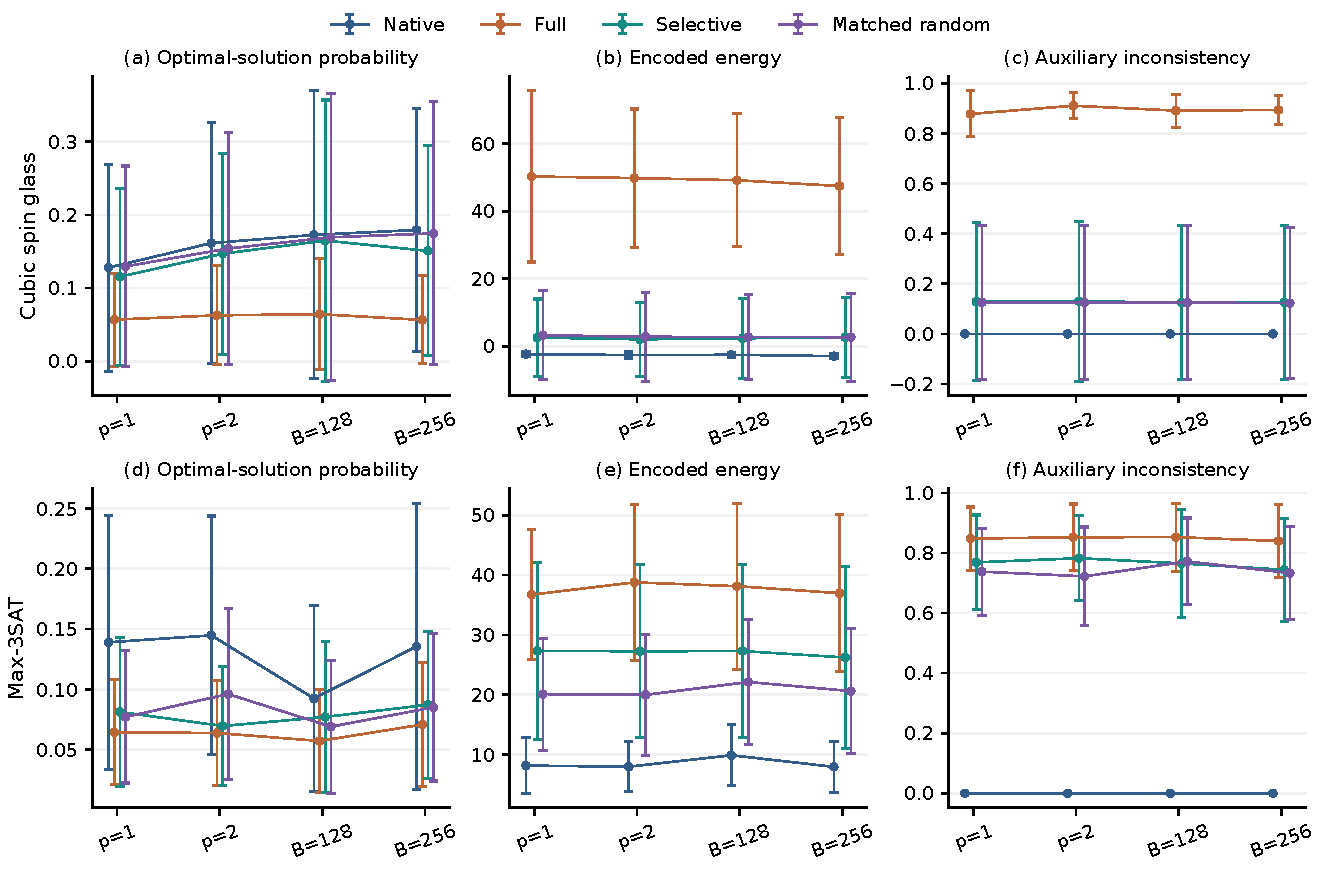
\includegraphics[width=\textwidth]{figure_e3_secondary_metrics.pdf}
    \caption{Additional noiseless-QAOA diagnostics recalculated from the frozen
    run rows. Panels (a)--(c) show spin-glass optimal-solution probability,
    encoded energy, and auxiliary inconsistency $R_{\mathrm{inc}}$;
    (d)--(f) show the same metrics
    for Max-3SAT.  Restarts and matched-random draws are averaged before the raw
    instance is used as the statistical unit.  Encoded energy is
    representation-specific and is shown only as a diagnostic.}
    \label{fig:e3-secondary-metrics}
\end{figure}
The encoded energies should not be compared as a performance ranking because
the four representations use different encoded Hamiltonians.  The stored field
\nolinkurl{auxiliary_inconsistency_rate} implements the event in
\cref{eq:rinc}: it is the probability mass, or sampled fraction, for which at
least one active auxiliary relation is violated.  It is therefore exactly
$1-P_{\mathrm{cons}}$ for the active auxiliary set.

\FloatBarrier
\subsection{Original and targeted warm-start diagnostics}
\label{app:results-warmstart}

The first sparse-RLT solve reported an optimum for all 14 QAOA instances
labelled as test. The saved vectors contain 96 original-variable pseudo-moments
and 292 pair pseudo-moments, for 388 diagnostic values in total.
After the selector repair, 62 distinct instance--representation/draw groups
have active auxiliaries. Their auxiliary warm-start probabilities are the
clipped pair pseudo-moments.

\Cref{fig:e4-signal-diagnostics} compares original-variable bias with pair
information. The pair pseudo-moments can differ from the independence closure;
this diagnostic alone does not establish a performance benefit.

\begin{figure}[!htbp]
    \centering
    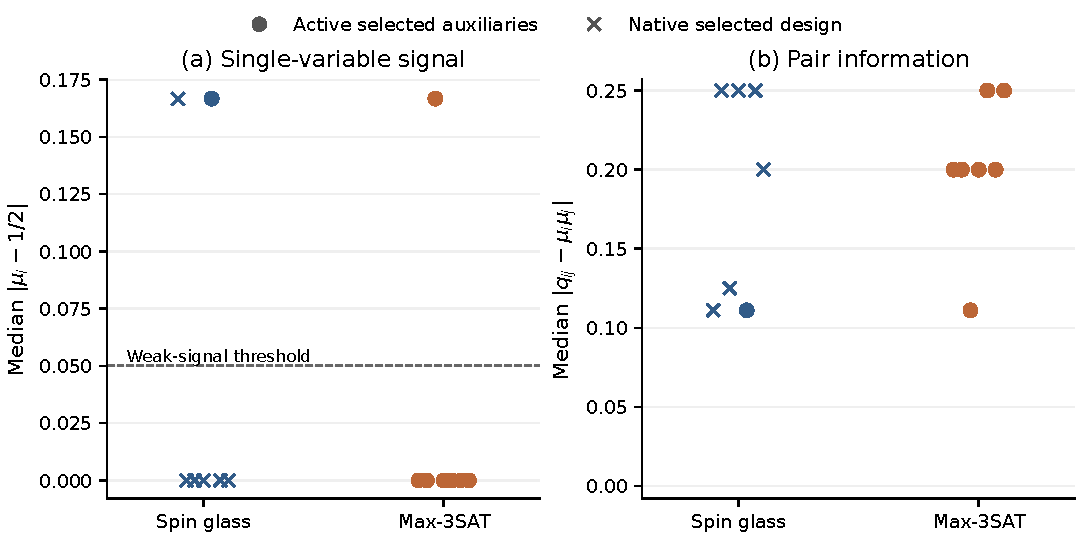
\includegraphics[width=\textwidth]{figure_e4_signal_diagnostics.pdf}
    \caption{Signal available to the E4 warm start.  Each point summarises one
    raw QAOA instance.  Circles identify cases where the repaired selected
    representation has active auxiliaries; crosses identify a native selected
    endpoint. The LP values are unchanged; design-status markers are updated.
    Eleven of fourteen instances have weak single-variable signal. Two
    instances combine stronger signal with an active selected auxiliary design.}
    \label{fig:e4-signal-diagnostics}
\end{figure}

Only three instances exceed the weak-signal threshold, and two belong to
the eight-case common selective active-auxiliary subset.
\Cref{tab:e4-warmstart-common} reports the corrected outcomes on this fixed
subset, after averaging three restarts per instance and keeping each budget
separate. Before the selector repair, the coordinate-corrected original E4 schedule
contained 4,320 rows.
Positive-depth, zero-depth, and all-scheduled summaries for the full design
set are separately available in the correction archive. The selector-repaired
merged schedule retains 4,176 rows after 144 redundant warm-policy rows for
newly zero-auxiliary designs are removed.

\begin{table}[!htbp]
\centering\footnotesize
\setlength{\tabcolsep}{3pt}
\caption{Coordinate-corrected original E4 results on the frozen common selective active-auxiliary subset. Cold is the mean original objective; other columns are paired differences from cold with exploratory, unadjusted 95\% Student-$t$ intervals across $n$ raw instances. $n_0$ counts zero-layer instances retained in the scheduled comparison. Negative differences favour warm starts. Pair uses archived clipped pair moments; Ind. multiplies clipped original probabilities without further clipping.}
\label{tab:e4-warmstart-common}
\resizebox{\textwidth}{!}{
\begin{tabular}{@{}lrrrlll@{}}
\toprule
Budget & $n$ & $n_0$ & Cold & Original-only minus cold & Pair minus cold & Ind. minus cold\\
\midrule
\multicolumn{7}{l}{\textbf{Spin glass}}\\
$p=1$ & 1 & 0 & $-1.093$ & $-0.715$ & $-0.647$ & $-0.681$\\
$p=2$ & 1 & 0 & $-1.722$ & $0.735$ & $-0.104$ & $0.164$\\
$B=128$ & 1 & 1 & $0.000$ & $-0.444$ & $-0.444$ & $-0.444$\\
$B=256$ & 1 & 0 & $-1.215$ & $0.290$ & $0.225$ & $0.307$\\
\addlinespace
\multicolumn{7}{l}{\textbf{Max-3SAT}}\\
$p=1$ & 7 & 0 & $10.035$ & $-0.562\;[-1.763,0.640]$ & $-0.872\;[-2.009,0.265]$ & $-0.552\;[-1.872,0.768]$\\
$p=2$ & 7 & 0 & $9.872$ & $-0.562\;[-1.741,0.616]$ & $-0.873\;[-2.154,0.408]$ & $-0.824\;[-2.036,0.387]$\\
$B=128$ & 7 & 2 & $9.884$ & $-0.647\;[-1.935,0.641]$ & $-0.677\;[-1.967,0.614]$ & $-0.808\;[-2.083,0.467]$\\
$B=256$ & 7 & 0 & $9.437$ & $-0.582\;[-1.795,0.632]$ & $-0.622\;[-1.879,0.635]$ & $-0.457\;[-2.034,1.121]$\\
\addlinespace
\bottomrule
\end{tabular}}
\end{table}

Spin-glass intervals are not estimable at $n=1$; all four Max-3SAT primary
pair-minus-cold intervals include zero. In the direct
pair-versus-original-only comparison, the Max-3SAT $p=2$ contrast is
$-0.311\;[-0.556,-0.065]$; the other such intervals and every
pair-versus-independence interval include zero. This secondary exploratory
contrast does not establish the primary pair-versus-cold claim.

\begin{figure}[!htbp]
\centering

\includegraphics[width=\textwidth]{figure_original_e4_warmstart_corrected.pdf}
\caption{Corrected original E4 pair-minus-cold differences on the selected
active-auxiliary subset. Error bars are exploratory instance-level 95\%
Student-$t$ intervals where estimable. The $n_0$ annotations identify retained
zero-layer instances; spin-glass crosses have $n=1$ and therefore no interval.}
\label{fig:e4-warmstart-corrected}
\end{figure}

\FloatBarrier
The targeted diagnostics and corrected warm-minus-cold plots below
complement \cref{tab:e4-strong-bias-warmstart}. The original screening
preceded QAOA evaluation; seven spin-glass and all ten Max-3SAT instances
exceed the signal threshold. Corrected mean optimal-solution probabilities
for targeted Max-3SAT under independence are $0.6094$ and $0.6224$ at
$p=1,2$, compared with $0.5987$ and $0.6262$ under pair warming.

\begin{figure}[!htbp]
    \centering
    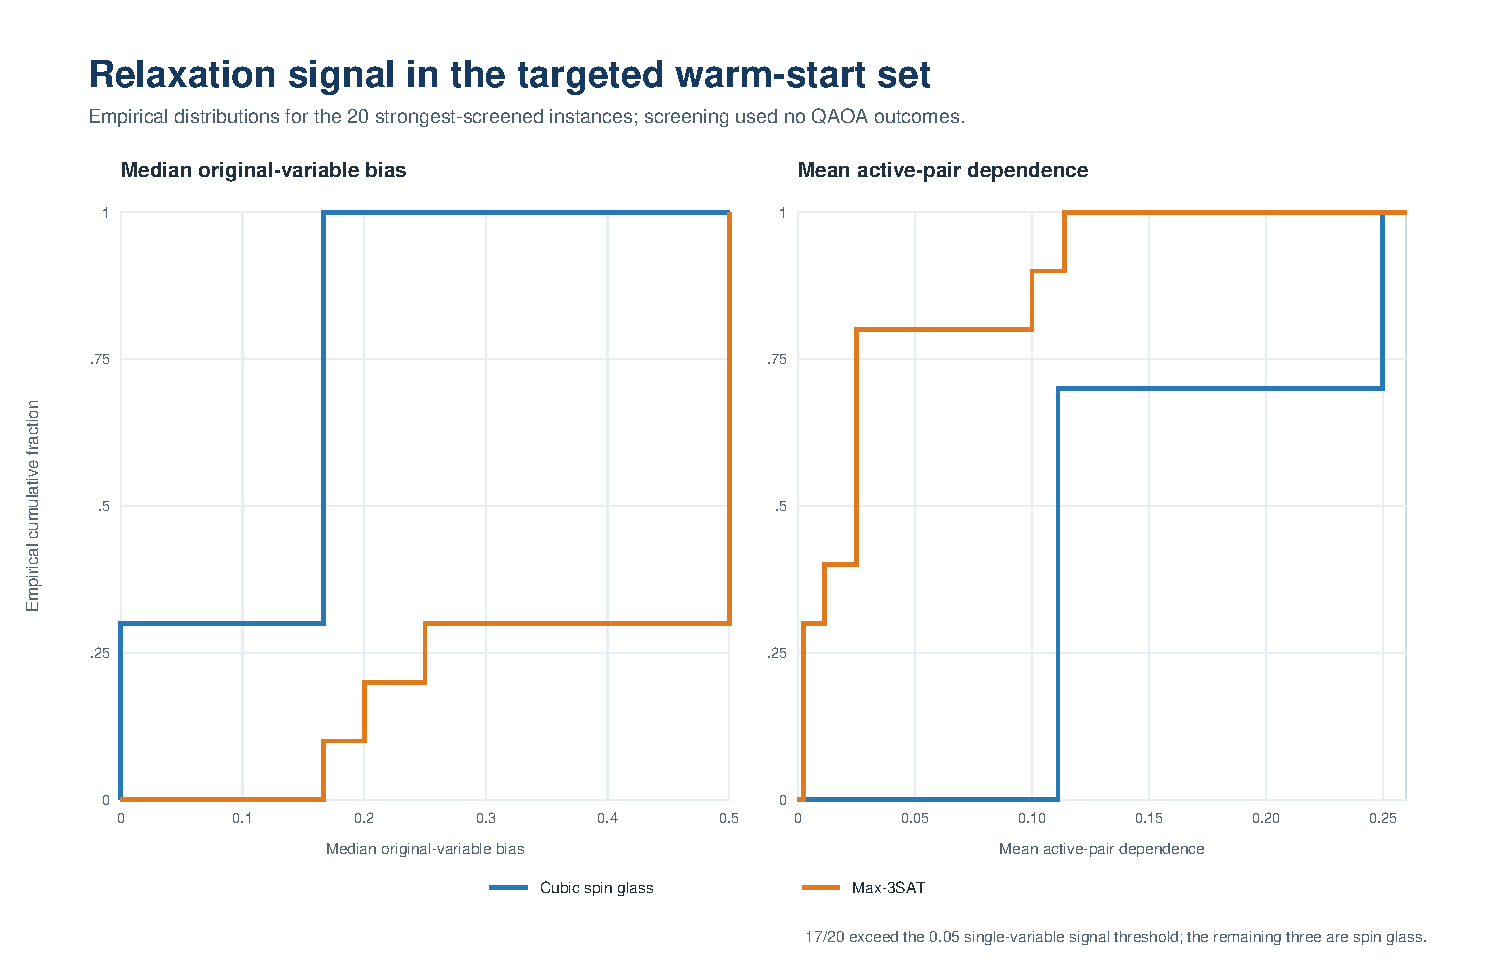
\includegraphics[width=\textwidth]
    {figure_strong_bias_marginals.pdf}
    \caption{Relaxation-signal diagnostics for the 20 strongest-screened
    instances: (a) original-variable bias and (b) pair dependence.  Screening used only relaxation quantities and was completed
    before any QAOA outcome was inspected.  Seven spin-glass and all ten
    Max-3SAT instances exceed the frozen single-variable signal threshold.}
    \label{fig:e4-strong-bias-marginals}
\end{figure}

\begin{figure}[!htbp]
\centering
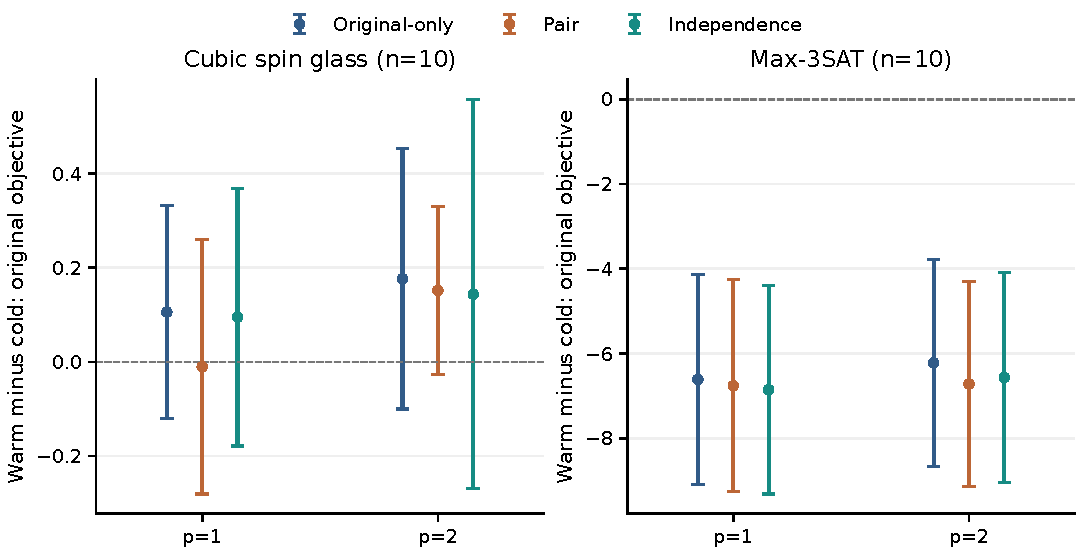
\includegraphics[width=\textwidth]{figure_strong_bias_warmstart.pdf}
\caption{Coordinate-corrected mean paired warm-minus-cold original-objective
differences on the fixed strongest-screened set: (a) spin glass and
(b) Max-3SAT. The three policies are shown separately. Error bars are
exploratory, unadjusted 95\% Student-$t$ intervals over ten raw instances per
family after averaging three restarts. Negative differences favour warm starts.}
\label{fig:e4-strong-bias-warmstart}
\end{figure}

\FloatBarrier

\subsection{Complete descriptive regime counts}
\label{app:results-regimes}

We next compared selective reduction with its auxiliary-count-matched random
control.  The planned endpoints were two-qubit depth, two-qubit gate count,
routing overhead, and QAOA objective.  Outcomes not meeting either directional interval criterion were assigned
to the residual (inconclusive) category; this does not establish equivalence.

\begin{table}[!htbp]
    \centering
    \small
    \caption{Help, residual (inconclusive), hurt and not-estimable counts for
    selective reduction relative to the matched-random control. The residual
    category includes uncertain intervals and does not establish equivalence.}
    \label{tab:e5-regime-summary}
    \begin{tabular}{@{}llrrrr@{}}
        \toprule
        Family & Endpoint & Help & Residual & Hurt & Not estimable\\
        \midrule
        Cubic spin glass & Two-qubit depth  & 8 & 17 & 0 & 11\\
        Cubic spin glass & Two-qubit gates  & 3 & 22 & 0 & 11\\
        Cubic spin glass & Routing overhead & 1 & 24 & 0 & 11\\
        Cubic spin glass & QAOA objective   & 1 & 25 & 2 & 0\\
        \addlinespace
        Max-3SAT & Two-qubit depth  & 20 & 0 & 0 & 16\\
        Max-3SAT & Two-qubit gates  & 19 & 1 & 0 & 16\\
        Max-3SAT & Routing overhead & 1 & 19 & 0 & 16\\
        Max-3SAT & QAOA objective   & 1 & 13 & 14 & 0\\
        \bottomrule
    \end{tabular}
\end{table}

Of 272 scheduled instance--metric endpoints, 191 were estimable: 54 helped,
121 were classified as residual (inconclusive) and 16 hurt; 81 were not estimable. In the

QAOA rows, each family contributes seven instances at four budgets.
Thirty-nine residual intervals extend beyond the tolerance band.
Classification follows
Appendix~\ref{app:experimental-statistics}; these are endpoint counts,
not independent-instance confidence statements.

The 81 not-estimable endpoints were expected sparse-device infeasibilities.
All-to-all data were estimable for all 18 instances in each family, while the
sparse-topology data were estimable for only seven of 18 spin-glass instances
and two of 18 Max-3SAT instances.  Some sparsity and pair-reuse bins also
contain only one or two observations.  The regime counts therefore show useful
patterns, but they are too small for a universal rule about problem structure.

\FloatBarrier
\subsection{Limited study with a representative noise model}
\label{sec:results-noise}

The 18-instance noise study follows the fixed simulator configuration in
Appendix~\ref{app:noise-protocol}. The tables below report absolute objectives,
degradation from each representation's own sampled noiseless baseline, and
paired selective-minus-native differences.

\begin{table}[!htbp]
    \centering
    \small
    \caption{Descriptive means in the limited noise study.  Lower objective
    values are better.  Degradation is the high-noise objective minus the
    noiseless objective.  The final column is the high-noise auxiliary
    inconsistency rate $R_{\mathrm{inc}}$ from \cref{eq:rinc}.}
    \label{tab:e6-noise-summary}
    \resizebox{\linewidth}{!}{
\begin{tabular}{@{}llrrrrr@{}}
        \toprule
        Family & Representation
        & Noiseless & Low noise & High noise
        & Degradation & Inconsistency\\
        \midrule
        Cubic spin glass
        & Native          & -3.052 & -0.699 & -0.087 & 2.965 & 0.000\\
        & Fully reduced   & -0.620 & -0.175 & -0.032 & 0.588 & 0.872\\
        & Selective       & -2.923 & -0.729 & -0.123 & 2.800 & 0.083\\
        & Matched random  & -2.953 & -0.769 & -0.124 & 2.829 & 0.082\\
        \addlinespace
        Max-3SAT
        & Native          & 7.953 & 9.305 & 9.700 & 1.748 & 0.000\\
        & Fully reduced   & 9.024 & 9.396 & 9.633 & 0.609 & 0.821\\
        & Selective       & 8.701 & 9.455 & 9.692 & 0.990 & 0.775\\
        & Matched random  & 8.402 & 9.302 & 9.642 & 1.239 & 0.771\\
        \bottomrule
    \end{tabular}}

\end{table}

Noise worsened every representation's mean original objective. Full reduction
changed least from its noiseless value, but started worse than native in both
families and retained high auxiliary inconsistency. Selective reduction had
lower inconsistency than full reduction for spin glass, but remained highly
inconsistent for Max-3SAT. Smaller degradation is not better absolute performance.

This table is descriptive.  The raw file contains three repeated rows per
instance for the native, fully reduced, and selective representations, and 15
rows for the five matched-random designs.  These repeated rows were therefore
averaged inside each raw instance before any uncertainty calculation.

\begin{table}[!htbp]
    \centering
    \small
    \caption{Instance-level selective-minus-native objective differences in
    the noise study.  Lower objective values are better, so a negative mean
    favours selective reduction.  The 95\% intervals are Student-$t$
    intervals across nine raw instances per family.  W/T/L gives the numbers
    of instance wins, ties, and losses using the predeclared 0.01 objective
    equivalence band.}
    \label{tab:e6-paired-noise}
    \begin{tabular}{@{}llrrrl@{}}
        \toprule
        Family & Noise & Mean difference & 95\% interval & $d_z$ & W/T/L\\
        \midrule
        Cubic spin glass & Noiseless & $0.129$  & $[-0.868,1.126]$ & $0.099$  & 5/0/4\\
                          & Low       & $-0.030$ & $[-0.312,0.251]$ & $-0.083$ & 6/0/3\\
                          & High      & $-0.036$ & $[-0.089,0.016]$ & $-0.532$ & 4/3/2\\
        \addlinespace
        Max-3SAT         & Noiseless & $0.749$  & $[0.140,1.358]$  & $0.945$  & 3/0/6\\
                          & Low       & $0.149$  & $[-0.046,0.344]$ & $0.589$  & 1/0/8\\
                          & High      & $-0.009$ & $[-0.133,0.116]$ & $-0.053$ & 5/0/4\\
        \bottomrule
    \end{tabular}
\end{table}

After within-instance aggregation, neither non-zero noise level showed a
clear selective advantage over native. All spin-glass intervals included zero;
Max-3SAT favoured native without noise and was inconclusive under noise.
The smaller Max-3SAT degradation starts from a worse noiseless baseline and
does not establish better absolute noisy performance. With nine instances
per family, this is an exploratory robustness check.


\FloatBarrier

\section{Five-seed compilation results}
\label{supp:multiseed-results}
These results use the same 30 Max-3SAT and 30 constructed instances as
the earlier cost-layer study. They are not new independent samples.
Main Section~\ref{sec:multiseed-methods} gives the methods and resource
definitions. Main Appendix~\ref{app:multiseed-audit} describes the saved
records and the independent checks.

\subsection{Budget points retained across seeds}
Table~\ref{tab:multiseed-retention} compares the new seed-1729 baseline
with the intersection of all five seed-specific TRUE sets.
Each entry pools the two synthesis strategies and 30 instances in its
family. TRUE means mixed-only within the saved candidate library.
It does not exclude full representations outside that library.
The same budget point must pass in each seed, but a different mixed
candidate may make it pass. Points share instances, so the large counts
are not large independent sample sizes.

\begin{table}[htbp]\centering\small
\caption{Mixed-only budget points within the saved library. The last
column divides the all-five-seed count by the new seed-1729 count.}
\label{tab:multiseed-retention}
\begin{tabular}{llrrr}\toprule
Family & Topology & Seed 1729 & All five seeds & Retained\\\midrule
Max-3SAT & Line-12 & 23,734 & 13,294 & 56.01\%\\
Max-3SAT & Ring-12 & 24,083 & 14,677 & 60.94\%\\
Max-3SAT & Grid-12 & 30,024 & 13,228 & 44.06\%\\
Constructed & Line-12 & 22,110 & 16,412 & 74.23\%\\
Constructed & Ring-12 & 7,946 & 6,683 & 84.11\%\\
Constructed & Grid-12 & 41,542 & 14,775 & 35.57\%\\\midrule
Pooled & & 149,439 & 79,069 & 52.91\%\\\bottomrule
\end{tabular}\end{table}

\begin{table}[htbp]\centering\small
\caption{Seed-specific results over 360 instance--topology--synthesis
settings. A setting has a region if at least one budget point is TRUE.
The settings share 60 instances. No point is UNKNOWN.}
\label{tab:multiseed-seeds}
\begin{tabular}{rrrr}\toprule
Seed & TRUE budget points & Settings with a region & Fraction\\\midrule
1729 & 149,439 & 255/360 & 70.83\%\\
2718 & 156,824 & 255/360 & 70.83\%\\
31415 & 155,289 & 262/360 & 72.78\%\\
57721 & 165,626 & 254/360 & 70.56\%\\
65537 & 155,638 & 256/360 & 71.11\%\\\bottomrule
\end{tabular}\end{table}

The total number of TRUE points can rise in another seed even when many
baseline points are lost: new points may appear elsewhere in the grid.
Thus similar totals do not show that the regions contain the same points.
There are $149{,}439-79{,}069=70{,}370$ baseline points that fail the TRUE
condition in at least one other seed.

\begin{figure}[htbp]\centering
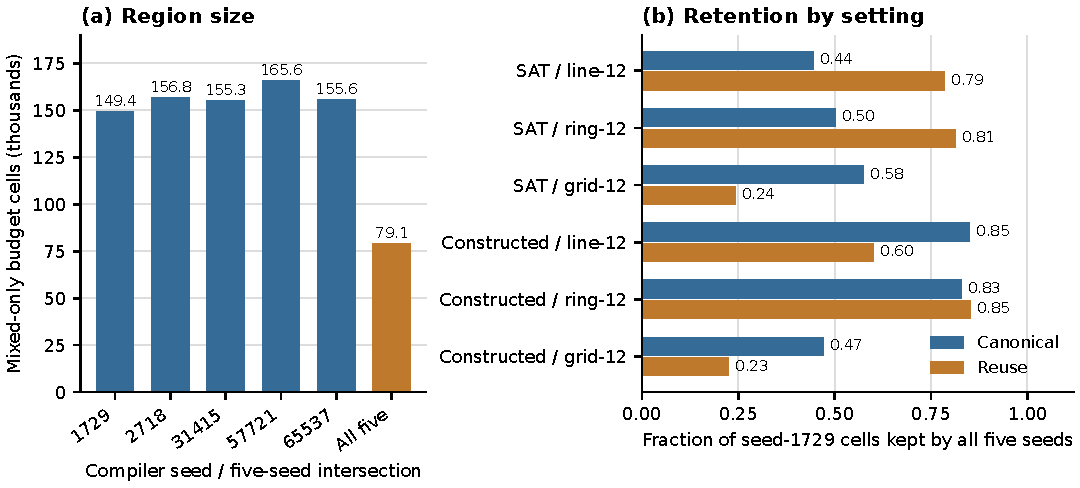
\includegraphics[width=\linewidth]{multiseed_si_corrected.pdf}
\caption{Five-seed compilation check within the saved candidate libraries.
(a) Number of mixed-only budget points for each seed, followed by their
intersection. (b) Fraction of new seed-1729 points retained by all five
seeds, shown separately for each family, topology and synthesis strategy.
SAT denotes weighted Max-3SAT. Each bar pools 30 instances. Points and
compiler settings share instances and are not independent samples.}
\label{fig:multiseed-checked}
\end{figure}

\subsection{Changes in regions, frontiers and selected candidates}
There are 360 instance--topology--synthesis settings. At least one common
mixed-only budget point survives all five seeds in 220 settings.
Having some common points does not mean that the whole region is unchanged.
Table~\ref{tab:multiseed-region-changes} separates these questions.
The earlier analysis labelled 158 changed regions as stable because it
counted points lost in every other seed rather than points lost in any
other seed. The table uses direct comparisons of the five complete sets.
A separate baseline-retention classification asks only whether the
seed-1729 TRUE points survive: 49 settings retain all baseline points,
171 retain some, 35 retain none of a nonempty baseline, and 105 have an
empty baseline. These four categories sum to 360. An unchanged baseline
can gain points in another seed, so the 49 baseline-stable settings are
not the same as the 15 settings with identical nonempty TRUE sets below.

\begin{table}[htbp]\centering\small
\caption{Region changes across the five seeds. The four rows partition
the 360 settings. The third row requires a nonempty seed-1729 region;
the last row includes any remaining change, including newly appearing regions.}
\label{tab:multiseed-region-changes}
\begin{tabular}{lr}\toprule
Relation between the five TRUE sets & Settings\\\midrule
Identical and nonempty & 15\\
Identical and empty & 81\\
Baseline nonempty, but no point common to all five & 35\\
All other changes & 229\\\bottomrule
\end{tabular}\end{table}

We also compare each of the four other seeds with seed 1729 in each
setting. This gives 1,440 paired comparisons, all based on the same 60
instances. The median Spearman correlation of candidate resource scores
is 0.970; the minimum is 0.765. The median Jaccard similarity of the
Pareto candidate sets is 0.667; the minimum is 0.125.
Thus score rankings often agree even when the Pareto sets change.
These summaries compare seeds within a synthesis strategy. They are
different from the comparisons between synthesis strategies in the main text.

The lowest-score candidate changes in 8 of the 1,440 comparisons.
This selector includes native and does not apply the four hard budgets.
At seed 1729, it chooses native in 353 of 360 settings and strictly mixed
in seven. No full representation is selected. The low winner-change rate
therefore mainly describes native choices; it is not evidence that mixed
choices are generally stable.

To complete the missing feasibility check, we keep the seed-1729 winner
fixed. We first record every point in the saved budget grid where its
seed-1729 circuit fits. We then use that candidate's saved circuits from
the other seeds to test those same points. In 320 of 1,440 comparisons it
loses at least one previously feasible point. This result explains why
keeping the same selected representation does not guarantee keeping its
feasible budget region. It is a grid-based diagnostic, not a result at
a newly chosen primary budget.

The corrected figure and tables were computed from the saved compiler
rows. They require no new compiler or QAOA calls. The correction script,
full setting-level tables and audit results accompany this revision.

\FloatBarrier\clearpage
\begin{thebibliography}{99}

\bibitem{BorosHammer2002}
Endre Boros and Peter~L. Hammer.
\newblock ``Pseudo-boolean optimization''.
\newblock \href{https://dx.doi.org/10.1016/S0166-218X(01)00341-9}{Discrete Applied Mathematics {\bf 123}, 155--225}~(2002).

\bibitem{Hadfield2021}
Stuart Hadfield.
\newblock ``On the representation of Boolean and real functions as Hamiltonians for quantum computing''.
\newblock \href{https://dx.doi.org/10.1145/3478519}{ACM Transactions on Quantum Computing {\bf 2}, Article 18, 1--21}~(2021).
\newblock \href{http://arxiv.org/abs/1804.09130}{arXiv:1804.09130}.

\bibitem{Farhi2014}
Edward Farhi, Jeffrey Goldstone, and Sam Gutmann.
\newblock ``A quantum approximate optimization algorithm''~(2014).
\newblock \href{http://arxiv.org/abs/1411.4028}{arXiv:1411.4028}.

\bibitem{Zhou2020}
Leo Zhou, Sheng-Tao Wang, Soonwon Choi, Hannes Pichler, and Mikhail D. Lukin.
\newblock ``Quantum Approximate Optimization Algorithm: Performance, Mechanism, and Implementation on Near-Term Devices''.
\newblock \href{https://doi.org/10.1103/physrevx.10.021067}{Physical Review X {\bf 10}, 021067}~(2020).

\bibitem{Glos2022}
Adam Glos, Aleksandra Krawiec, and Zolt{\'a}n Zimbor{\'a}s.
\newblock ``Space-efficient binary optimization for variational quantum computing''.
\newblock \href{https://dx.doi.org/10.1038/s41534-022-00546-y}{npj Quantum Information {\bf 8}, 39}~(2022).
\newblock \href{http://arxiv.org/abs/2009.07309}{arXiv:2009.07309}.

\bibitem{CampbellDahl2022}
Colin Campbell and Edward Dahl.
\newblock ``QAOA of the highest order''.
\newblock In 2022 IEEE 19th International Conference on Software Architecture Companion (ICSA-C), pages 141--146~(2022).
\newblock \href{https://dx.doi.org/10.1109/ICSA-C54293.2022.00035}{doi:10.1109/ICSA-C54293.2022.00035}.
\newblock \href{http://arxiv.org/abs/2111.12754}{arXiv:2111.12754}.

\bibitem{Stein2023}
Jonas Stein, Farbod Chamanian, Maximilian Zorn, Jonas N{\"u}{\ss}lein, Sebastian Zielinski, Michael K{\"o}lle, and Claudia Linnhoff-Popien.
\newblock ``Evidence that PUBO outperforms QUBO when solving continuous optimization problems with the QAOA''.
\newblock In Proceedings of the Genetic and Evolutionary Computation Conference Companion.
\newblock \href{https://dx.doi.org/10.1145/3583133.3596358}{Pages 2254--2262}~(2023).
\newblock \href{http://arxiv.org/abs/2305.03390}{arXiv:2305.03390}.

\bibitem{Bell2025}
Kristina Bell, Adam Lowe, Emily Coles, Nathanael Ridgway, and Gillian Marshall.
\newblock ``A comparison of quadratic and higher-order representations for QAOA''~(2025).
\newblock \href{http://arxiv.org/abs/2509.20127}{arXiv:2509.20127}.

\bibitem{Verchere2023}
Zo{\'e} Verch{\`e}re, Sourour Elloumi, and Andrea Simonetto.
\newblock ``Optimizing variational circuits for higher-order binary optimization''.
\newblock In 2023 IEEE International Conference on Quantum Computing and Engineering (QCE), volume 1, pages 19--25~(2023).
\newblock \href{https://dx.doi.org/10.1109/QCE57702.2023.00011}{doi:10.1109/QCE57702.2023.00011}.
\newblock \href{http://arxiv.org/abs/2307.16756}{arXiv:2307.16756}.

\bibitem{Weidenfeller2022}
Johannes Weidenfeller, Lucia~C. Valor, Julien Gacon, Caroline Tornow, Luciano Bello, Stefan Woerner, and Daniel~J. Egger.
\newblock ``Scaling of the quantum approximate optimization algorithm on superconducting qubit based hardware''.
\newblock \href{https://dx.doi.org/10.22331/q-2022-12-07-870}{Quantum {\bf 6}, 870}~(2022).
\newblock \href{http://arxiv.org/abs/2202.03459}{arXiv:2202.03459}.

\bibitem{Harrigan2021}
Matthew P. Harrigan et al.
\newblock ``Quantum approximate optimization of non-planar graph problems on a planar superconducting processor''.
\newblock \href{https://doi.org/10.1038/s41567-020-01105-y}{Nature Physics {\bf 17}, 332--336}~(2021).

\bibitem{Rosenberg1975}
I.~G. Rosenberg.
\newblock ``Reduction of bivalent maximization to the quadratic case''.
\newblock Cahiers du Centre d'\'Etudes de Recherche Op\'erationnelle {\bf 17}, 71--74~(1975).

\bibitem{BorosGruber2014}
Endre Boros and Aritanan Gruber.
\newblock ``On quadratization of pseudo-boolean functions''~(2014).
\newblock \href{http://arxiv.org/abs/1404.6538}{arXiv:1404.6538}.

\bibitem{Dattani2019}
Nike Dattani.
\newblock ``Quadratization in discrete optimization and quantum mechanics''~(2019).
\newblock \href{http://arxiv.org/abs/1901.04405}{arXiv:1901.04405}.

\bibitem{FreedmanDrineas2005}
Daniel Freedman and Petros Drineas.
\newblock ``Energy minimization via graph cuts: Settling what is possible''.
\newblock In 2005 IEEE Computer Society Conference on Computer Vision and Pattern Recognition (CVPR'05), volume 2, pages 939--946~(2005).
\newblock \href{https://dx.doi.org/10.1109/CVPR.2005.143}{doi:10.1109/CVPR.2005.143}.

\bibitem{Ishikawa2011}
Hiroshi Ishikawa.
\newblock ``Transformation of general binary MRF minimization to the first-order case''.
\newblock \href{https://dx.doi.org/10.1109/TPAMI.2010.91}{IEEE Transactions on Pattern Analysis and Machine Intelligence {\bf 33}, 1234--1249}~(2011).

\bibitem{AnthonyEtAl2017}
Martin Anthony, Endre Boros, Yves Crama, and Aritanan Gruber.
\newblock ``Quadratic reformulations of nonlinear binary optimization problems''.
\newblock \href{https://dx.doi.org/10.1007/s10107-016-1032-4}{Mathematical Programming {\bf 162}, 115--144}~(2017).

\bibitem{Anthony2016}
Martin Anthony, Endre Boros, Yves Crama, and Aritanan Gruber.
\newblock ``Quadratization of symmetric pseudo-Boolean functions''.
\newblock \href{https://doi.org/10.1016/j.dam.2016.01.001}{Discrete Applied Mathematics {\bf 203}, 1--12}~(2016).

\bibitem{BorosCramaRodriguezHeck2020}
Endre Boros, Yves Crama, and Elisabeth Rodr{\'i}guez-Heck.
\newblock ``Compact quadratizations for pseudo-Boolean functions''.
\newblock \href{https://dx.doi.org/10.1007/s10878-019-00511-0}{Journal of Combinatorial Optimization {\bf 39}, 687--707}~(2020).

\bibitem{VermaLewis2020}
Amit Verma and Mark Lewis.
\newblock ``Optimal quadratic reformulations of fourth degree pseudo-Boolean functions''.
\newblock \href{https://dx.doi.org/10.1007/s11590-019-01460-7}{Optimization Letters {\bf 14}, 1557--1569}~(2020).

\bibitem{VermaLewisKochenberger2021}
Amit Verma, Mark Lewis, and Gary Kochenberger.
\newblock ``Efficient QUBO transformation for higher degree pseudo Boolean functions''~(2021).
\newblock \href{http://arxiv.org/abs/2107.11695}{arXiv:2107.11695}.

\bibitem{CramaEtAl2025}
Yves Crama, Sourour Elloumi, Am{\'e}lie Lambert, and Elisabeth Rodr{\'i}guez-Heck.
\newblock ``Quadratization and convexification in polynomial binary optimization''.
\newblock \href{https://dx.doi.org/10.1007/s10878-025-01334-y}{Journal of Combinatorial Optimization {\bf 50}, Article 28}~(2025).

\bibitem{Herrman2021}
Rebekah Herrman, Lorna Treffert, James Ostrowski, Phillip~C. Lotshaw, Travis~S. Humble, and George Siopsis.
\newblock ``Globally optimizing QAOA circuit depth for constrained optimization problems''.
\newblock \href{https://dx.doi.org/10.3390/a14100294}{Algorithms {\bf 14}, 294}~(2021).
\newblock \href{http://arxiv.org/abs/2108.03281}{arXiv:2108.03281}.

\bibitem{Schmidbauer2024}
Lukas Schmidbauer, Karen Wintersperger, Elisabeth Lobe, and Wolfgang Mauerer.
\newblock ``Polynomial reduction methods and their impact on QAOA circuits''.
\newblock In 2024 IEEE International Conference on Quantum Software (QSW), pages 35--45~(2024).
\newblock \href{https://dx.doi.org/10.1109/QSW62656.2024.00018}{doi:10.1109/QSW62656.2024.00018}.
\newblock \href{http://arxiv.org/abs/2406.08889}{arXiv:2406.08889}.

\bibitem{Schmidbauer2026}
Lukas Schmidbauer, Elisabeth Lobe, Ina Schaefer, and Wolfgang Mauerer.
\newblock ``It's quick to be square: Fast quadratisation for quantum toolchains''.
\newblock \href{https://dx.doi.org/10.1145/3800943}{ACM Transactions on Quantum Computing {\bf 7}, Article 18, 1--46}~(2026).
\newblock \href{http://arxiv.org/abs/2411.19934}{arXiv:2411.19934}.

\bibitem{Rovara2026}
Damian Rovara, Lukas Burgholzer, and Robert Wille.
\newblock ``Quantum hardware-efficient selection of auxiliary variables for QUBO formulations''.
\newblock In 2026 Design, Automation \& Test in Europe Conference (DATE), pages 1--7~(2026).
\newblock \href{https://dx.doi.org/10.23919/DATE69613.2026.11539407}{doi:10.23919/DATE69613.2026.11539407}.
\newblock \href{http://arxiv.org/abs/2511.19613}{arXiv:2511.19613}.

\bibitem{Dragoi2026}
Sabina Dr{\u a}goi, Alberto Baiardi, and Daniel~J. Egger.
\newblock ``Approximate quadratization of high-order Hamiltonians for combinatorial quantum optimization''.
\newblock Physical Review Research {\bf 8}, 023159~(2026).
\newblock \href{http://arxiv.org/abs/2505.04700}{arXiv:2505.04700}.

\bibitem{Egger2021}
Daniel~J. Egger, Jakub Mare{\v c}ek, and Stefan Woerner.
\newblock ``Warm-starting quantum optimization''.
\newblock \href{https://dx.doi.org/10.22331/q-2021-06-17-479}{Quantum {\bf 5}, 479}~(2021).

\bibitem{TateSDP2023}
Reuben Tate, Majid Farhadi, Creston Herold, Greg Mohler, and Swati Gupta.
\newblock ``Bridging classical and quantum with SDP initialized warm-starts for QAOA''.
\newblock \href{https://dx.doi.org/10.1145/3549554}{ACM Transactions on Quantum Computing {\bf 4}, Article 9, 1--39}~(2023).

\bibitem{TateCustom2023}
Reuben Tate, Jai Moondra, Bryan Gard, Greg Mohler, and Swati Gupta.
\newblock ``Warm-started QAOA with custom mixers provably converges and computationally beats Goemans--Williamson's Max-Cut at low circuit depths''.
\newblock \href{https://dx.doi.org/10.22331/q-2023-09-26-1121}{Quantum {\bf 7}, 1121}~(2023).

\bibitem{WangMaxCut2018}
Zhihui Wang, Stuart Hadfield, Zhang Jiang, and Eleanor G. Rieffel.
\newblock ``Quantum approximate optimization algorithm for MaxCut: A fermionic view''.
\newblock \href{https://doi.org/10.1103/physreva.97.022304}{Physical Review A {\bf 97}, 022304}~(2018).

\bibitem{FarhiLocal2020}
Edward Farhi, David Gamarnik, and Sam Gutmann.
\newblock ``The Quantum Approximate Optimization Algorithm Needs to See the Whole Graph: Worst Case Examples''.
\newblock Preprint at \href{https://arxiv.org/abs/2005.08747}{arXiv:2005.08747}~(2020).

\bibitem{Akshay2020}
V. Akshay, H. Philathong, M. E. S. Morales, and J. D. Biamonte.
\newblock ``Reachability Deficits in Quantum Approximate Optimization''.
\newblock \href{https://doi.org/10.1103/physrevlett.124.090504}{Physical Review Letters {\bf 124}, 090504}~(2020).

\bibitem{Cain2023}
Madelyn Cain, Edward Farhi, Sam Gutmann, Daniel Ranard, and Eugene Tang.
\newblock ``The QAOA gets stuck starting from a good classical string''.
\newblock Preprint at \href{https://arxiv.org/abs/2207.05089v2}{arXiv:2207.05089v2}~(2023).

\bibitem{LandDoig1960}
A. H. Land and A. G. Doig.
\newblock ``An Automatic Method of Solving Discrete Programming Problems''.
\newblock \href{https://doi.org/10.2307/1910129}{Econometrica {\bf 28}, 497--520}~(1960).

\bibitem{LawlerWood1966}
E. L. Lawler and D. E. Wood.
\newblock ``Branch-and-Bound Methods: A Survey''.
\newblock \href{https://doi.org/10.1287/opre.14.4.699}{Operations Research {\bf 14}, 699--719}~(1966).

\bibitem{Hadfield2019}
Stuart Hadfield, Zhihui Wang, Bryan O'Gorman, Eleanor G. Rieffel, Davide Venturelli, and Rupak Biswas.
\newblock ``From the Quantum Approximate Optimization Algorithm to a Quantum Alternating Operator Ansatz''.
\newblock \href{https://doi.org/10.3390/a12020034}{Algorithms {\bf 12}, 34}~(2019).

\bibitem{Powell1994}
M. J. D. Powell.
\newblock ``A Direct Search Optimization Method That Models the Objective and Constraint Functions by Linear Interpolation''.
\newblock \href{https://doi.org/10.1007/978-94-015-8330-5_4}{In Advances in Optimization and Numerical Analysis, pages 51--67}~(1994).

\bibitem{Student1908}
Student.
\newblock ``The Probable Error of a Mean''.
\newblock \href{https://doi.org/10.2307/2331554}{Biometrika {\bf 6}, 1--25}~(1908).

\bibitem{Lucas2014}
Andrew Lucas.
\newblock ``Ising formulations of many NP problems''.
\newblock \href{https://doi.org/10.3389/fphy.2014.00005}{Frontiers in Physics {\bf 2}, 5}~(2014).

\bibitem{Glover2018}
Fred Glover, Gary Kochenberger, and Yu Du.
\newblock ``A Tutorial on Formulating and Using QUBO Models''.
\newblock Preprint at \href{https://arxiv.org/abs/1811.11538}{arXiv:1811.11538}~(2018).

\bibitem{CowtanPhase2020}
Alexander Cowtan, Silas Dilkes, Ross Duncan, Will Simmons, and Seyon Sivarajah.
\newblock ``Phase Gadget Synthesis for Shallow Circuits''.
\newblock \href{https://doi.org/10.4204/eptcs.318.13}{Electronic Proceedings in Theoretical Computer Science {\bf 318}, 213--228}~(2020).

\bibitem{CowtanUCC2020}
Alexander Cowtan, Will Simmons, and Ross Duncan.
\newblock ``A Generic Compilation Strategy for the Unitary Coupled Cluster Ansatz''.
\newblock Preprint at \href{https://arxiv.org/abs/2007.10515}{arXiv:2007.10515}~(2020).

\bibitem{Murali2019}
Prakash Murali, Jonathan M. Baker, Ali Javadi-Abhari, Frederic T. Chong, and Margaret Martonosi.
\newblock ``Noise-Adaptive Compiler Mappings for Noisy Intermediate-Scale Quantum Computers''.
\newblock \href{https://doi.org/10.1145/3297858.3304075}{Proceedings of the Twenty-Fourth International Conference on Architectural Support for Programming Languages and Operating Systems, 1015--1029}~(2019).

\bibitem{DebEtAl2002}
Kalyanmoy Deb, Amrit Pratap, Sameer Agarwal, and T.~Meyarivan.
\newblock ``A fast and elitist multiobjective genetic algorithm: NSGA-II''.
\newblock \href{https://dx.doi.org/10.1109/4235.996017}{IEEE Transactions on Evolutionary Computation {\bf 6}, 182--197}~(2002).

\bibitem{Basso2022}
Joao Basso, David Gamarnik, Song Mei, and Leo Zhou.
\newblock ``Performance and limitations of the QAOA at constant levels on large sparse hypergraphs and spin glass models''.
\newblock In 2022 IEEE 63rd Annual Symposium on Foundations of Computer Science (FOCS), pages 335--343~(2022).
\newblock \href{https://dx.doi.org/10.1109/FOCS54457.2022.00039}{doi:10.1109/FOCS54457.2022.00039}.
\newblock \href{http://arxiv.org/abs/2204.10306}{arXiv:2204.10306}.

\bibitem{PelofskeShortDepth2024}
Elijah Pelofske, Andreas B{\"a}rtschi, and Stephan Eidenbenz.
\newblock ``Short-depth QAOA circuits and quantum annealing on higher-order Ising models''.
\newblock \href{https://dx.doi.org/10.1038/s41534-024-00825-w}{npj Quantum Information {\bf 10}, 30}~(2024).

\bibitem{Pelofske2024}
Elijah Pelofske, Andreas B{\"a}rtschi, Lukasz Cincio, John Golden, and Stephan Eidenbenz.
\newblock ``Scaling whole-chip QAOA for higher-order Ising spin glass models on heavy-hex graphs''.
\newblock \href{https://dx.doi.org/10.1038/s41534-024-00906-w}{npj Quantum Information {\bf 10}, 109}~(2024).
\newblock \href{http://arxiv.org/abs/2312.00997}{arXiv:2312.00997}.

\bibitem{Qiskit2024}
Ali Javadi-Abhari et al.
\newblock ``Quantum computing with Qiskit''.
\newblock Preprint at \href{https://arxiv.org/abs/2405.08810}{arXiv:2405.08810}~(2024).

\bibitem{Virtanen2020}
Pauli Virtanen et al.
\newblock ``SciPy 1.0: fundamental algorithms for scientific computing in Python''.
\newblock \href{https://doi.org/10.1038/s41592-019-0686-2}{Nature Methods {\bf 17}, 261--272}~(2020).

\bibitem{Li2019}
Gushu Li, Yufei Ding, and Yuan Xie.
\newblock ``Tackling the Qubit Mapping Problem for NISQ-Era Quantum Devices''.
\newblock \href{https://doi.org/10.1145/3297858.3304023}{Proceedings of the Twenty-Fourth International Conference on Architectural Support for Programming Languages and Operating Systems, 1001--1014}~(2019).

\bibitem{Crooks2018}
Gavin E. Crooks.
\newblock ``Performance of the Quantum Approximate Optimization Algorithm on the Maximum Cut Problem''.
\newblock Preprint at \href{https://arxiv.org/abs/1811.08419}{arXiv:1811.08419}~(2018).

\bibitem{Sack2021}
Stefan H. Sack and Maksym Serbyn.
\newblock ``Quantum annealing initialization of the quantum approximate optimization algorithm''.
\newblock \href{https://doi.org/10.22331/q-2021-07-01-491}{Quantum {\bf 5}, 491}~(2021).

\bibitem{HuangfuHall2018}
Q. Huangfu and J. A. J. Hall.
\newblock ``Parallelizing the dual revised simplex method''.
\newblock \href{https://doi.org/10.1007/s12532-017-0130-5}{Mathematical Programming Computation {\bf 10}, 119--142}~(2018).

\bibitem{Marshall2020}
Jeffrey Marshall, Filip Wudarski, Stuart Hadfield, and Tad Hogg.
\newblock ``Characterizing local noise in QAOA circuits''.
\newblock \href{https://doi.org/10.1088/2633-1357/abb0d7}{IOP SciNotes {\bf 1}, 025208}~(2020).

\bibitem{WangNoise2021}
Samson Wang et al.
\newblock ``Noise-induced barren plateaus in variational quantum algorithms''.
\newblock \href{https://doi.org/10.1038/s41467-021-27045-6}{Nature Communications {\bf 12}, 6961}~(2021).

\bibitem{Franca2021}
Daniel Stilck França and Raul García-Patrón.
\newblock ``Limitations of optimization algorithms on noisy quantum devices''.
\newblock \href{https://doi.org/10.1038/s41567-021-01356-3}{Nature Physics {\bf 17}, 1221--1227}~(2021).

\bibitem{Nagies2025}
Sebastian Nagies, Kevin~T. Geier, Javed Akram, Dimitrios Bantounas, Michael Johanning, and Philipp Hauke.
\newblock ``Boosting quantum annealing performance through direct polynomial unconstrained binary optimization''.
\newblock \href{https://dx.doi.org/10.1088/2058-9565/adcae6}{Quantum Science and Technology {\bf 10}, 035008}~(2025).
\newblock \href{http://arxiv.org/abs/2412.04398}{arXiv:2412.04398}.

\bibitem{Nusslein2023}
Jonas N{\"u}{\ss}lein, Sebastian Zielinski, Thomas Gabor, Claudia Linnhoff-Popien, and Sebastian Feld.
\newblock ``Solving (Max) 3-SAT via quadratic unconstrained binary optimization''~(2023).
\newblock \href{http://arxiv.org/abs/2302.03536}{arXiv:2302.03536}.

\bibitem{Wurtz2021}
Jonathan Wurtz and Peter Love.
\newblock ``MaxCut quantum approximate optimization algorithm performance guarantees for $p>1$''.
\newblock \href{https://doi.org/10.1103/physreva.103.042612}{Physical Review A {\bf 103}, 042612}~(2021).

\bibitem{BassoHighDepth2022}
Joao Basso, Edward Farhi, Kunal Marwaha, Benjamin Villalonga, and Leo Zhou.
\newblock ``The Quantum Approximate Optimization Algorithm at High Depth for MaxCut on Large-Girth Regular Graphs and the Sherrington-Kirkpatrick Model''.
\newblock \href{https://doi.org/10.4230/lipics.tqc.2022.7}{Leibniz International Proceedings in Informatics (TQC 2022) {\bf 232}, 7:1--7:21}~(2022).

\bibitem{SheraliAdams1990}
Hanif D. Sherali and Warren P. Adams.
\newblock ``A Hierarchy of Relaxations between the Continuous and Convex Hull Representations for Zero-One Programming Problems''.
\newblock \href{https://doi.org/10.1137/0403036}{SIAM Journal on Discrete Mathematics {\bf 3}, 411--430}~(1990).

\bibitem{McCormick1976}
Garth P. McCormick.
\newblock ``Computability of global solutions to factorable nonconvex programs: Part I --- Convex underestimating problems''.
\newblock \href{https://doi.org/10.1007/bf01580665}{Mathematical Programming {\bf 10}, 147--175}~(1976).
\end{thebibliography}

\end{document}
